\documentclass[a4paper]{article}

% LANGAGE
\input{../latex-std/lang-de.tex}
\input{../latex-std/lang-de-extensions.tex}

% DOCUMENT PRE POST META
\input{../latex-std/doc-pre-post.tex}

\input{../latex-std/doc-biber.tex}
\addbibresource{bibliography.bib}


% TEXT STRUCTURE ENVIRONMENTS
\input{../latex-std/articul-comments.tex}
\input{../latex-std/articul-structure.tex}


% MATH SYMBOLS
\input{../latex-std/symb-math.tex}

\newcommand{\mc}{Markow-Kette}
\title{Effiziente Berechnung von Varianzen in \mc{}n}%und stabile
\author{Maximilian Starke}
\affil{Fakultät für Informatik, Technische Universität Dresden}
\date{\today}

\usepackage{mathtools}
\usepackage{ragged2e}

\usepackage{framed}
\usepackage{amsmath, amssymb}
\usepackage{tabularx}

\DeclareMathOperator*{\argmin}{\arg\min}

\usepackage{pgfplots}
\pgfplotsset{width=10cm,compat=1.10}
\usepgfplotslibrary{fillbetween}
\newcolumntype{P}[1]{>{\centering\arraybackslash}p{#1}}

\usepackage{listings}

\newcolumntype{M}[1]{>{\centering\arraybackslash}m{#1}}
\newcolumntype{L}[1]{>{\flushleft\arraybackslash}m{#1}}


\usepackage{tikz}

\usetikzlibrary{%
	arrows,
	shapes,
	shapes.misc,% wg. rounded rectangle
	shapes.arrows,%
	chains,%
	matrix,%
	positioning,% wg. " of "
	backgrounds,
	fit,
	petri,
	scopes,%
	decorations.pathmorphing,% /pgf/decoration/random steps | erste Graphik
	shadows,%
	calc
}
%#1
\tikzstyle{vertex}=[circle, minimum size=20pt, line width = 1pt, draw = black]
\tikzstyle{target} = [vertex, double, double distance = 1pt]
\tikzstyle{edge} = [draw,shorten > = 1pt, shorten < = 1pt, line width=1pt,->]
\tikzstyle{medge} = [draw, line width = 8pt, yellow!50]
\tikzstyle{weight} = [font=\small]
\tikzstyle{selected edge} = [draw,line width=5pt,-,red!50]
\tikzstyle{ignored edge} = [draw,line width=5pt,-,black!20]

\usepackage{relsize}

\usepackage{xcolor}
% maybe install minted some day and make syntax highlighting###

\usepackage[utf8]{inputenc}
\usepackage{amsmath, amssymb}

\usepackage[thmmarks,amsmath,hyperref,noconfig]{ntheorem} 
% erlaubt es, Sätze, Definitionen etc. einfach durchzunummerieren.
\newtheorem{satz}{Satz}[section] % Nummerierung nach Abschnitten
\newtheorem{proposition}[satz]{Proposition}
\newtheorem{korollar}[satz]{Korollar}
\newtheorem{lemma}[satz]{Lemma}
\newtheorem{vermutung}[satz]{Vermutung}

\theorembodyfont{\upshape}
\newtheorem{beispiel}[satz]{Beispiel}
\newtheorem{bemerkung}[satz]{Bemerkung}
\newtheorem{definition}[satz]{Definition} %[section]
\newtheorem{algorithmus}[satz]{Algorithmus}

\theoremstyle{nonumberplain}
\theoremheaderfont{\itshape}
\theorembodyfont{\normalfont}
\theoremseparator{.}
\theoremsymbol{\ensuremath{_\Box}}
\newtheorem{beweis}{Beweis}
\newtheorem{beweiss}{Beweisskizze}

\qedsymbol{\ensuremath{_\Box}}

\usepackage{chngcntr}
\counterwithin{figure}{section}

\tikzstyle{block} = [rectangle, draw, fill=blue!40, 
text width=7em, text centered, rounded corners, minimum height=5em, node distance= 4.5cm, line width = 2pt]


\tikzstyle{cblock} = [rectangle, draw, fill=blue!40, 
text width=7em, text centered, rounded corners, minimum height=5em, node distance= 3.0cm, line width = 2pt]


\tikzstyle{line} = [draw, -latex', line width = 1pt]


\tikzstyle{cloud} = [ fill = white, rectangle, draw, rounded corners, node distance=2cm,
minimum height=2.5em]

\pgfdeclarelayer{bg}
%\pgfsetlayers{bg,main}	

\pgfdeclarelayer{foreground}
\pgfdeclarelayer{background}
% tell TikZ how to stack them (back to front)
\pgfsetlayers{bg,background,main,foreground}

\newenvironment{meta}
{\begin{center} \Large \color{red} META: \hspace{2ex} \large \color{blue}}
	{\end{center}}

\begin{document}

% title page:
\maketitle
\vspace{3em}
\tableofcontents
\pagebreak

\section{Einführung}

Zur Analyse relevanter Zielgrößen in probabilistischen Systemen sind \mc{}n mit Kantengewichten ein wesentliches, häufig genutztes Modell. Mit dessen Hilfe kann beispielsweise die Dauer eines Verbindungsaufbaus in Netzwerken modelliert werden. Wir wollen in dieser Arbeit Varianzen akkumulierter Kantengewichte auf endlichen Pfaden in \mc{}n bis zum Erreichen einer Menge von Zielzuständen und deren effiziente Berechnung betrachten.
Während Erwartungswerte der akkumulierten Kantengewichte in der wissenschaftlichen Literatur bereits ausführlich untersucht worden sind, trifft dies nicht auf die Varianzen zu, obgleich diese besonders in sicherheitskritischen Systemen oder zur Beurteilung von Risiken durch Abweichung von der Erwartung besondere Relevanz erhalten.
Verhoeff \cite{Verh04} trug praktische Anwendungen zusammen, von denen wir hier zwei erläutern wollen:

Die niederländische Regierung entschied einst in Bezug auf Probleme mit hohem Verkehrsaufkommen, anstatt auf möglichst geringe Erwartungswerte der Fahrtzeit hinzuwirken, eher die Minimierung der Varianz der Fahrtzeit in den Fokus zu nehmen. Auf diese Weise ist man im Durchschnitt zwar länger unterwegs, erreicht aber mehr Planungssicherheit, kann also Ankunftszeiten genauer vorhersagen:
Wenn wir mit einer gewissen Wahrscheinlichkeit $\geq p$ rechtzeitig an einem Ort ankommen möchten, dann subtrahieren wir von der gewünschten Ankunftszeit den Erwartungswert der Fahrtdauer und einen Zeitpuffer, welcher wesentlich von der Varianz abhängt.

In der Wirtschaft kommt es immer wieder vor, dass Budgets für bestimmte Ausgaben geplant werden. Insofern größere Abweichungen der Kosten nach oben unbedingt zu vermeiden sind, kann es von Vorteil sein, anstatt eine Investition in Höhe von fiktiven 1000\euro{} zu planen, bei der mit 300\euro{} Abweichung der tatsächlichen Kosten gerechnet werden muss, eine alternative Investition zum selben Zweck .in Höhe von erwarteten 1100\euro{} anzustreben, bei welcher eine Abweichung von nur 50\euro{} erwartet wird.


Verhoeff präsentierte lineare Gleichungssysteme für die Berechnung von Varianzen und Kovarianzen \cite{Verh04}. Wir werden zunächst die erforderlichen Grundlagen zu Wahrscheinlichkeitstheorie sowie \mc{}n für den Leser darlegen. Anschließend werden wir einen Algorithmus zur Berechnung von Varianzen und Kovarianzen akkumulierter Kantengewichte formal herleiten. Wir werden  die Betrachtungen von Verhoeff insbesondere um eine ausführliche Herleitung für die Berechnung von Kovarianzen erweitern und zeigen, dass alle ermittelten Gleichungssysteme tatsächlich eindeutig lösbar sind. Danach werden wir eine Implementation des hergeleiteten Algorithmus' hinsichtlich ihrer Performance analysieren. Zum Abschluss werden wir noch einmal den Blick auf Markow-Entscheidungsprozesse lenken und uns der Problemstellung widmen, wie Varianzen minimiert werden können.

\section{Grundlagen}

\subsection{Wahrscheinlichkeitstheorie}

\newcommand{\probspace}{diskreter Wahr\-schein\-lich\-keits\-raum}
\newcommand{\probspacen}{diskreten Wahr\-schein\-lich\-keits\-raum}
\newcommand{\probspaceexraw}{(\Omega, P)}
\newcommand{\probspaceex}{$(\Omega, P)$}
\begin{definition}[\probspace{}] \label{def-probspace}
	\hspace{-0.5em} Wir nennen ein Paar \probspaceex{} einen \probspacen{}, wenn $\Omega$ eine abzählbare Menge ist und $P : \Omega \to [0,1] $ eine Funktion mit
	\begin{equation}
		\sum_{\omega \in \Omega} P(\omega) = 1 \text{.}
	\end{equation} Wir nennen $\Omega$ in diesem Zusammenhang auch Ergebnismenge und $P$ eine Wahr\-schein\-lich\-keitsverteilung auf $\Omega$.
\end{definition}
\newcommand{\rvar}{Zufallsvariable}
\begin{definition}[\rvar{}] \label{def-rvar}
	Sei \probspaceex{} ein \probspace{}. Eine Funktion $X : \Omega \to \mathbb{R}$ heißt \rvar{} auf \probspaceex{}. Wir nennen $X$ auch kurz \rvar{}, falls der Kontext \probspaceex{} klar ist.
\end{definition}
\newcommand{\expect}{Erwartungswert}
\newcommand{\mexp}{\mathcal{E}}
\begin{definition}[\expect{}] \label{def-expect}
	\hspace{1ex} Sei \probspaceex{} ein \probspace{} und $X$ eine \rvar{} auf \probspaceex{}. Mit
	\begin{equation}
		\mathcal{E}_{\probspaceexraw{}}(X) \coloneqq \sum_{\omega \in \Omega}{P(\omega) \cdot X(\omega)}
	\end{equation}
	bezeichnen wir den \expect{} von $X$ auf \probspaceex{}. Sollte der Kontext \probspaceex{} klar sein, schreiben wir auch kurz $\mathcal{E}(X)$. Es sei angemerkt, dass es für $|\Omega|=\infty$ Fälle gibt, bei denen die Summe nicht beschränkt ist. Wir schreiben dafür $\mathcal{E}(X) = \infty$ bzw. $\mathcal{E}(X) = -\infty$ und sagen, dass der Erwartungswert nicht existiert.
\end{definition}
\begin{beispiel}
	Seien $\Omega = \mathbb{N}_{>0}$, $P : \Omega \to [0,1] : n \mapsto 2^{-n}$ und $R : \Omega \to \mathbb{R} : n \mapsto 2^{n}$. Dann gibt es offensichtlich für jede Zahl $a \in \mathbb{R}$ eine endliche Teilmenge von $T \subseteq \Omega$ mit $\sum_{n \in T}{P(n) \cdot R(n)} \geq a$. Dazu wählen wir einfach $T \coloneqq \{n \in \mathbb{N}_{>0}\mid n \leq \lceil a \rceil \}$ und erhalten $\sum_{n \in T}{P(n) \cdot R(n)} = |T| = \lceil a \rceil \leq \mathcal{E}(R)$. Damit erhalten wir $\mathcal{E}(R) = \infty$.
\end{beispiel}
Wir werden uns im Folgenden nur auf \rvar n beziehen, für welche ein Erwartungswert existiert.
\begin{beispiel}\label{example-expect}
	Ein manipulierter Spielwürfel habe 6 Seiten $\Omega = \{1,2,3,4,5,6\}$, wobei die $1$ im Vergleich zu einem herkömmlichen Würfel mit einer $2$ überklebt wurde. Dies drücken wir durch die Zufallsvariable $X : \Omega \to \mathbb{R} : s \mapsto \max(2,s)$ aus. Außerdem wurde der Würfel mit ungleichmäßig verteilter Masse so gefertigt, dass nach einem Wurf nicht alle Seiten gleich wahrscheinlich oben liegen. Wir nehmen für dieses Beispiel eine Wahrscheinlichkeitsverteilung mit $P(1)=0,1$, $P(2)=0,15$, $P(3)=0,15$, $P(4)=0,15$, $P(5)=0,15$, $P(6)=0,3$ an.
	Dann ist eine Augenzahl pro Wurf von
	\[
	\mathcal{E}(X) = (0,1 + 0,15) \cdot 2 + 0,15 \cdot (3 + 4 + 5) + 0,3 \cdot 6 = 4,1
	\]
	zu erwarten und damit $0,6$ Augen mehr als bei einem ungezinkten Würfel mit \expect{} $3,5$. Würden wir nun alle beschrifteten Zahlen noch zusätzlich quadrieren, erhielten wir einen Würfel mit $Y : \Omega \to \mathbb{R} : s \mapsto \max(4, s^2)$ und würden im Schnitt $19,3$ Augen bei einem Wurf erwarten:
	\[
	\mathcal{E}(Y) = (0,25) \cdot 4 + 0,15 \cdot (9 + 16 + 25) + 0,3 \cdot 36 = 19,3
	\]
\end{beispiel}

Es lässt sich leicht die folgende Linearität des \expect{}es beobachten:

\begin{lemma} \label{lem-explin}
 Seien $X$, $Y$ Zufallsvariablen auf demselben \probspace{}, $c,d \in \mathbb{R}$. Dann gilt:
\begin{equation}
		\mathcal{E}(X + cY + d) = \mathcal{E}(X) + c \mathcal{E}(Y) + d \label{eq-linearity}
\end{equation}
Dabei ist  $X + cY + d$ die übliche Notation für die \rvar{} gegeben durch $Z : \Omega \to \mathbb{R} : \omega \mapsto X(\omega) + c \cdot Y(\omega)+ d$.
\end{lemma}
\begin{beweis}
\begin{align}
	\mathcal{E}(X + cY + d) & = \sum_{\omega \in \Omega}{P(\omega) \cdot (X + cY + d)(\omega) } \nonumber \\
	& = \sum_{\omega \in \Omega}{P(\omega) \cdot X(\omega) + c \cdot P(\omega) \cdot Y(\omega) + d \cdot P(\omega)} \nonumber \\
	& = \mathcal{E}(X) + c \mathcal{E}(Y) + d \nonumber
\end{align}
\end{beweis}
\newcommand{\var}{Varianz}
\newcommand{\mvar}{\mathcal{V}\!ar}
\begin{definition}[\var]\label{def-var}
	Sei \probspaceex{} ein \probspace{} und $X$ eine \rvar{} auf \probspaceex{}. Mit
	\begin{equation}
		\mvar_{\probspaceexraw{}}(X) \coloneqq  \mathcal{E}_{\probspaceexraw{}}\left(\left(X - \mathcal{E}_{\probspaceexraw{}} (X)\right)^{2}\right)
	\end{equation}
	bezeichnen wir die \var{} von $X$ auf  \probspaceex{}. Sollte der Kontext \probspaceex{} klar sein, schreiben wir kurz $\mvar(X)$.
\end{definition}
\newcommand{\cov}{Kovarianz}
\newcommand{\mcov}{\mathcal{C}\!ov}
\begin{definition}[\cov]\label{def-cov}
	Seien \probspaceex{} ein \probspace{} und $X, Y$ \rvar n auf \probspaceex{}. Die \cov{} $\mcov{}_{\probspaceexraw}(X,Y)$ ist definiert durch:
	\begin{equation}
		\mcov{}_{\probspaceexraw}(X,Y) \coloneqq \mathcal{E} \Big( \big(X - \mathcal{E}(X)\big)\big(Y - \mathcal{E}(Y) \big)\Big)
	\end{equation}
\end{definition}

Offensichtlich ist die \var{} ein Spezialfall der \cov{}, denn aus den Definitionen folgt unmittelbar $\mvar_{\probspaceexraw}(X) = \mcov{}_{\probspaceexraw}(X,X)$. Wir betrachten im Folgenden, wie sich Kovarianzen durch Erwartungswerte beschreiben lassen.

\begin{lemma}\label{lemma-cov-exp}
	Seien $X$ und $Y$ \rvar{}n auf demselben \probspace{}. Dann gilt:
\begin{equation}
	\mcov{}(X,Y) = \mathcal{E}(XY) - \mathcal{E}(X)\mathcal{E}(Y)
\end{equation}
\end{lemma}
\begin{beweis}
\begin{align*}
\mcov{}(X,Y) & = \mathcal{E}\big( \left(X - \mathcal{E}(X)\right)\left(Y - \mathcal{E}(Y)\right)\big) && \text{(Definition \ref{def-cov})} \\
& = \mathcal{E}\big(XY - X \mathcal{E}(Y) - Y \mathcal{E}(X) + \mathcal{E}(X)\mathcal{E}(Y)\big) \\
& = \mathcal{E}(XY) - 2 \mathcal{E}(X) \mathcal{E}(Y) + \mathcal{E}(X) \mathcal{E}(Y) && \text{(Lemma \ref{lem-explin})}\\
& = \mathcal{E}(XY) - \mathcal{E}(X)\mathcal{E}(Y) \\
\end{align*}
\end{beweis}

Betrachten wir den Spezialfall $X = Y$  von Lemma \ref{lemma-cov-exp}, dann erhalten wir folgende Beziehung für \var{}en:

\begin{korollar}\label{kor-var-exp}
	Sei $X$ eine \rvar{} auf einem \probspace{}. Dann gilt:
	\begin{equation}
		\mvar(X) = \mathcal{E}(X^{2}) - \mathcal{E}\left(X\right)^{2}
	\end{equation}
\end{korollar}
%\begin{beweis}
%	\begin{align*}
%		\mvar(X) & = \mathcal{E}\left( \left(X - \mathcal{E}(X)\right)^{2}\right) && \text{(Definition \ref{def-var})} \\
%		& = \mathcal{E}(X^{2} - 2 X \mathcal{E}(X) + \mathcal{E}(X)^{2}) \\
%		& = \mathcal{E}(X^2) - 2 \mathcal{E}(X) \mathcal{E}(X) + \mathcal{E}(X)^{2} && \text{(Linearität (\ref{eq-linearity}))}\\
%		& = \mathcal{E}(X^{2}) - \mathcal{E}\left(X\right)^{2} \\
% 	\end{align*}
%\end{beweis}
Ähnlich zur Linearität von \expect{}en (\ref{eq-linearity}) lässt sich für \var{}en folgende Beziehung feststellen:
\begin{lemma}\label{lemma-var-qlinear}
	Sei $X$ eine \rvar{} auf einem \probspace{}, $c,d \in \mathbb{R}$. Dann gilt:
	\begin{equation}
		\mvar(cX + d) = c^2\cdot\mvar(X)
	\end{equation}
\end{lemma}
\begin{beweis}
\begin{align*}
\mvar(cX + d) & = \mathcal{E}\Big(\big(cX + d - \mathcal{E}(cX + d)\big)^2\Big) && \text{(Defintion \ref{def-var})} \\
& = \mathcal{E}\Big(\big(cX + d - c\mathcal{E}(X) - d\big)^2\Big) && \text{(Lemma \ref{lem-explin}}\\
& = \mathcal{E}\Big(c^2 \cdot \big(X - \mathcal{E}(X) \big)^2\Big)\\
& = c^2 \cdot \mathcal{E}\Big( \big(X - \mathcal{E}(X) \big)^2\Big) && \text{(Lemma \ref{lem-explin}}\\
& = c^2 \cdot \mvar(X) && \text{(Defintion \ref{def-var})}
\end{align*}
\end{beweis}
Entsprechend der Intuition ist die Varianz, das Quadrat der Standardabweichung, invariant unter Addition einer Konstanten zur \rvar{}. Wird jedoch die \rvar{} mit einem Faktor skaliert, so ändert sich die Varianz um das Quadrat des Faktors. Aus gutem Grund wird die Varianz auch mittlere quadratische Abweichung genannt.


Durch das Wegfallen von $d$ lässt sich recht trivial auf Gleichungen schließen, welche unter Umständen nicht mehr auf dem ersten Blick als klar und offensichtlich angesehen werden können. Das folgende Korollar soll dies verdeutlichen:
\begin{korollar}
	Sei $X$ eine Zufallsvariable und $c \in \mathbb{R}$. Dann gilt:
	\begin{equation}
		\mathcal{E}\left((c+X)^2\right) = (c+ \mathcal{E}(X))^2 + \mvar(X)
	\end{equation}
\end{korollar}
\begin{beweis}
Aus Korollar \ref{kor-var-exp} folgt unmittelbar \[\mvar(X+c) = \mathcal{E}\left((X+c)^{2}\right) - \left(\mathcal{E}\left(X+c\right)\right)^{2}\text{.}\] Die linke Seite kann nach Lemma \ref{lemma-var-qlinear} vereinfacht werden zu $\mvar(X+c) = \mvar(X)$. Der Subtrahend $\left(\mathcal{E}\left(X+c\right)\right)^{2}$ lässt sich aufgrund der Linearität (Lemma \ref{lem-explin}) auch als $\left( \mathcal{E}(X)+c\right)^{2}$ 
schreiben.
\end{beweis}

\begin{beispiel}
	Wir wollen nun Beispiel \ref{example-expect} fortsetzen. 
	Nach Korollar \ref{kor-var-exp} beträgt die \var{} beim ursprünglichen Würfel also $\mvar(X) = \mathcal{E}(X^2) - \mathcal{E}(X)^2 = \mathcal{E}(Y) - \mathcal{E}(X)^2 = 19,3 - 16,81 = 2,49$. Es sei bemerkt, dass wir $Y$ geschickt so gewählt haben, dass $Y = X^2$ gilt. Und tatsächlich ergibt die Berechnung nach Definition \ref{def-var} denselben Wert:
	\begin{align*}
	\mvar(X) & = 0,15 \cdot \big((3- 4,1)^2 + (4-4,1)^2 + (5-4,1)^2\big) + && \\
	& \hspace{1.2em} + 0,25 \cdot (2 - 4,1)^2 + 0,3 \cdot (6-4,1)^2 && \\
	& = 0,25 \cdot 4,41 + 0,15 \cdot \big(1,21 + 0,01 + 0,81\big) + 0,3 \cdot 3,61 && \\
	& = 2,49 &&
	\end{align*}
	Die \cov{} lässt sich nach Lemma \ref{lemma-cov-exp} berechnen als $\mcov(X,Y) = \mathcal{E}(XY) - \mathcal{E}(X)\mathcal{E}(Y)$.
	Wir kennen bereits $\mathcal{E}(X)$ sowie $\mathcal{E}(Y)$ und es gilt:
	\[
		\mexp(XY) = \mexp(X^3) = 0,25 \cdot 2^3 + 0,15 \cdot (3^3 + 4^3 + 5^3) + 0.3 \cdot 6^3 = 99.2
	\]
	Dann ist  $\mcov(X,Y) = 99.2 - 4,1 \cdot 19,3 = 20.07$ und tatsächlich ergibt die explizite Rechnung denselben Wert:
	\begin{align*}
		\mcov(X,Y) &= \mathcal{E} \Big( \big(X - \mathcal{E}(X)\big)\big(Y - \mathcal{E}(Y) \big)\Big) \\
		&= 0,25 \cdot (2-4,1)(4-19,3) \\
		& \hspace{1.2em} + 0,15 \cdot (3-4,1)(9-19,3) + 0,15 \cdot (4-4.1)(16-19,3) \\
		& \hspace{1.2em} +  0,15 \cdot (5-4,1)(25-19,3)) + 0.3 \cdot (6-4,1)(36-19,3) \\
		&= 20.07
	\end{align*}
\end{beispiel}

\subsection{\mc{}n}

\newcommand{\mcex}{$M = (Q, P, I)$}
\begin{definition}[\mc]\label{def-mc}
	Eine \mc{} ist ein Tupel $(Q, P, I)$ mit den Eigenschaften
	\begin{enumerate}[(a)]
		\item $Q$ ist eine abzählbare Menge.
		\item $P : Q \times Q \to [0,1]$ mit der Eigenschaft $\forall q \in Q : \sum_{q' \in Q}{P(q,q') = 1}$.
		\item $I : Q \to [0,1]$ ist eine Wahrscheinlichkeitsverteilung auf $Q$.
	\end{enumerate}	
	Die Bilder von $P$ nennen wir auch Transitionswahrscheinlichkeiten und definieren mit welcher Wahrscheinlichkeit, nämlich $P(q,q')$ vom aktuellen Zustand $q$ in den Zustand $q'$ übergegangen wird. $I$ ist die initiale Verteilung, welche definiert, mit welcher Wahrscheinlichkeit ein Zustand als Startzustand gewählt wird.
\end{definition}

Für theoretische Betrachtungen ist es durchaus sinnvoll unendliche \mc{}n zu betrachten. Wir werden uns jedoch auf endliche beschränken, d.h. $|Q| < \infty$, sobald wir zur Berechnung von u.a. Varianzen entsprechende Gleichungssysteme herleiten. Andernfalls bestünde das Gleichungssystem aus unendlich vielen Gleichungen in unendlich vielen Variablen.

\newcommand{\gpath}{Pfad}
\newcommand{\pfin}{\mathrm{Paths}}%_{fin}
\begin{definition}[\gpath]\label{def-path}
	Sei \mcex{} eine \mc{}. Die Menge aller endlichen \gpath e in $M$ sei definiert durch
	\begin{equation}
		\pfin(M) \coloneqq \{p \in Q^{k} \mid k \in \mathbb{N}_{>0} \land \forall 0 \leq i < k : P(p_i,p_{i+1}) > 0\}
	\end{equation}
	Wir bezeichnen mit $|p|$ die Größe des Tupels $p$, d.h. $|p| = k$ für $p \in Q^k$. Wir beginnen Indizes bei $0$.
	Die Wahrscheinlichkeit $\mathrm{\tilde{P}}(p)$ eines Pfades ist gegeben durch
	\begin{equation}
		\mathrm{\tilde{P}}(p) \coloneqq \prod_{i = 0}^{|p| - 2}{P(p_i,p_{i+1})}
	\end{equation}
	Insbesondere ist $\mathrm{\tilde{P}}(p) = 1$ für alle Pfade $p$ mit $|p| = 1$. Für Tupel $p \in Q^k$, $k \in \mathbb{N}_{>0}$, die keine Pfade sind, gilt entsprechend $\mathrm{\tilde{P}}(p) = 0$.
	
	Für $|p| = 2$ entspricht die Wahrscheinlichkeit $\mathrm{\tilde{P}}(p)$ genau der Wahrscheinlichkeit gegeben durch die Funktion $P$, nämlich der Transitionswahrscheinlichkeit aus der \mc{}. $\mathrm{\tilde{P}}$ ergibt sich als eindeutige Fortsetzung von $P$, es gilt $P = \mathrm{\tilde{P}}\vert_{Q\times Q}$, und wir schreiben daher im Folgenden einfach nur $P$.
\end{definition}

\newcommand{\reward}{Gewichtsfunktion}
\begin{definition}[\reward]
	Sei \mcex{} eine \mc{}. Eine \reward{} auf $M$ ist eine Abbildung
	\begin{equation}
	R : Q \times Q \to \mathbb{R}\text{.}
	\end{equation} 
\end{definition}
Wir bezeichnen Gewichtsfunktionen typischerweise mit $R$ in Anlehnung an das englische Wort \textit{reward}.
Offenbar gibt es analog zur Wahrscheinlichkeit $P$ eine eindeutige Fortsetzung für eine \reward{} $R$ auf Pfade, gegeben durch Aufsummierung aller Kantengewichte entlang eines solchen:
\begin{equation}
	\mathrm{\tilde{R}} : \bigcup_{k \in \mathbb{N}_{>0}}{Q^k} \to \mathbb{R} : p \mapsto \sum_{i = 0}^{|p| - 2}{R(p_i,p_{i+1})}
\end{equation}
Wir schreiben im Folgenden einfach $R$.
\begin{definition}\label{def-path-to}
	Sei \mcex{} eine \mc{}, $s \in Q$ ein beliebiger Zustand, genannt Startzustand, und $A \subseteq Q$ eine Menge von Zielzuständen. Wir bezeichnen die Menge der Pfade, welche in $s$ starten und in $A$ enden, jedoch $A$ nicht zwischenzeitlich schon erreichen, mit:
	\begin{equation}
		\pfin_{s \rightarrow A}(M) \coloneqq \{ p \in \pfin(M) \mid p_0 = s \land p_{|p|-1} \in A \land \forall i < |p| - 1 : p_i \notin A \}
	\end{equation}
	
\end{definition}

Wir ziehen nun Erkenntnisse heran, die Baier und Katoen in Kapitel 10.1 ihres Buches \textit{Principles of Model Checking} \cite{Bai08} beschreiben, speziell im Abschnitt \textit{Reachability Probabilities}.
Setzen wir einmal voraus, dass von jedem Zustand $q\in Q$, welcher von $s$ erreichbar ist, ein Pfad in die Zielzustandsmenge $A$ existiert, das heißt
\[
\pfin_{s \rightarrow \{q\}}(M) \neq \emptyset  \quad \Rightarrow \quad \pfin_{q \rightarrow A}(M) \neq \emptyset \text{.}
\]
 Unter dieser Voraussetzung beobachteten Baier und Katoen, dass es ein fast sicheres Ereignis ist, nach endlich vielen Übergängen an einem Zustand aus $A$ vorbeizukommen.
Die endlichen Pfade, welche wir ausschließlich betrachten wollen, lassen sich als Präfixe der unendlichen Pfade $\mathrm{Paths}_{inf}(s) \coloneqq \{p \in Q^\omega \mid p(0) = s \land \forall i \in \mathbb{N}: P(p_i,p_{i+1})>0 \}$ der \mc{} auffassen.
Man sieht leicht, dass sich ein endlicher Pfad mit der Menge an jenen unendlichen Pfaden identifizieren lässt, welche diesen als  Präfix haben.
Eine Menge endlicher Pfade ist abzählbar, da wir die Pfade als endliche Wörter über dem Alphabet bestehend aus den Zuständen auffassen können.
Nach dieser Beobachtung ist dann
\[
(\mathrm{Paths}_{s \rightarrow A}(M), P)
\] ein \probspace{}, da die Menge aller Pfade, welche $A$ nie besuchen, ein fast unmögliches Ereignis darstellt. Die Fortsetzung von $R$ ist eine \rvar{} auf $\mathrm{Paths}_{s \rightarrow A}(M)$. 
\begin{beispiel} \label{example-mc}
	Gegeben sei eine \mc{} \mcex{} mit
	\begin{align*}
	Q &=\{1,2,3,4,5,6\} \\
	P &=\begin{pmatrix}
	0 & 0,5 & 0,5 & 0 & 0 & 0 \\
	0 & 0 & 0 & 0 & 0 & 1 \\
	0 & 0,25 & 0 & 0,5 & 0,25 & 0 \\
	0 & 0 & 0 & 0,8 & 0,2 & 0 \\
	0 & 0 & 0 & 0 & 0 & 1 \\
	0 & 0 & 0 & 0 & 1 & 0 \\
	\end{pmatrix} \\
	I &=\begin{pmatrix} 1 & 0 & 0 & 0 & 0 & 0\end{pmatrix}^\intercal
	\end{align*}
	Wir betrachten also eine \mc{} mit dem einzigen initialen Zustand $1$. Weiterhin sei $\{5,6\}$ die betrachtete Menge an Zielzuständen, welche wir auf Pfaden erreichen wollen.	
	Eine \mc{} lässt sich immer auch als Graph auffassen: Wir beschriften alle Kanten $(i,j)$ mit Übergangswahrscheinlichkeit und Wert der Gewichtsfunktion $R$ in der Schreibweise $P(i,j) : R(i,j)$. Sei die Gewichtsfunktion $R$ implizit definiert durch folgenden Graphen:
	\begin{center}%#2
		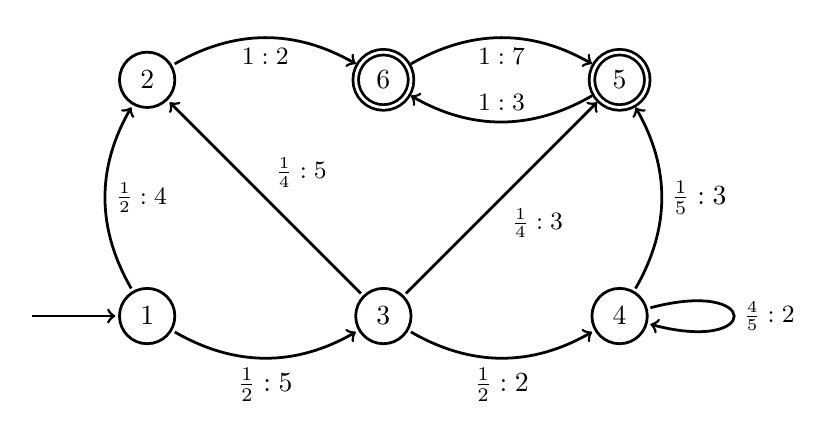
\begin{tikzpicture}[auto,swap,scale=3]
		
		% First we draw the vertices
		\foreach \pos/\name in {{(0,0)/1}, {(1,0)/3}, {(2,0)/4}, {(0,1)/2}}
		\node[vertex] (\name) at \pos {$\name$};
		
		% First we draw the vertices
		\foreach \pos/\name in {{(1,1)/6}, {(2,1)/5}}
		\node[target] (\name) at \pos {$\name$};
		
		% Connect vertices with edges and draw weights
		\foreach \source/ \dest /\weight in {
			1/2/{\frac{1}{2}:4},
			2/6/{1:2},
			5/6/{1:3},
			6/5/{1:7}
		}
		\path[edge] (\source) to[bend left] node[weight]{$\weight$} (\dest);
		
		% Connect vertices with edges and draw weights
		\foreach \source/ \dest /\weight in {
			1/3/{\frac{1}{2}:5},
			3/4/{\frac{1}{2}:2},
			4/5/{\frac{1}{5}:3}
		}
		\path[edge] (\source) to[bend right] node{$\weight$} (\dest);
		
		% Connect vertices with edges and draw weights
		\foreach \source/ \dest /\weight in {
			3/2/{\frac{1}{4}:5},
			3/5/{\frac{1}{4}:3}
		}
		\path[edge] (\source) to node[weight]{$\weight$} (\dest);
		
		\foreach \source/ \dest /\weight in {
			4/4/{\frac{4}{5}:2}
		}
		\path[edge] (\source) to[loop right] node[weight]{$\weight$} (\dest);
		
		% Draw initial state
		\path[edge] (-0.5,0) to (1);
		
		\end{tikzpicture}
	\end{center}
	Wir wollen nun zur Veranschaulichung den Erwartungswert und die Varianz von $R$ im Wahrscheinlichkeitsraum $(\mathrm{Paths}_{1 \rightarrow \{5,6\}}(M), P)$ betrachten. Die von $5$ beziehungsweise $6$ ausgehenden Kanten samt Beschriftung sind für diesen Fall irrelevant. Die Tupel aus $Q^n$ können wir mit Wörtern über dem Alphabet $Q$ identifizieren. Wir erhalten so:
	\begin{equation*}
	\Omega \coloneqq \mathrm{Paths}_{1 \rightarrow \{5,6\}}(M) = \big\{126,1326,135\big\} \; \cup \big\{134^n5 \in Q^{n+3} \mid n\geq 1\big\} 
	\end{equation*}
	Für den Erwartungswert $\mathcal{E}(R)$ ergibt sich:
	\newcommand{\exres}{10}
	\begin{align*}
	\mathcal{E}(R) & = \sum_{p \in \Omega}{P(p) \cdot R(p)}\\
	& = \frac{1}{2}\cdot 6_{\scriptscriptstyle [126]} + \frac{1}{8}\cdot 12_{\scriptscriptstyle [1326]} + \frac{1}{8}\cdot 8_{\scriptscriptstyle [135]} + \sum_{n = 0}^{\infty}{\frac{1}{20}\cdot\left(\frac{4}{5}\right)^n \cdot (10 + 2n)}_{\scriptscriptstyle [134^n5]} \\
	& = \exres{}
	\end{align*}
	Für das Berechnen der unendlichen Summe möchten wir an dieser Stelle auf den Appendix verweisen. Mit Korollar \ref{kor-geosum} und \ref{kor-infsum} und der Zerlegung
	\begin{equation*}
		\sum_{n = 0}^{\infty}{\frac{1}{20}\cdot\left(\frac{4}{5}\right)^n \cdot (10 + 2n)}
		= \frac{1}{2}\sum_{n = 0}^{\infty}{\left(\frac{4}{5}\right)^n} + \frac{1}{10} \sum_{n = 0}^{\infty}{\left(\frac{4}{5}\right)^n \cdot n}
	\end{equation*}
	lässt sich der Wert dieser Summe, nämlich $4,5$, leicht ausrechnen.
	Als Varianz $\mvar(R)$ erhalten wir, diesmal unter Verwendung von Korollar \ref{kor-infqsum}:
	\begin{align*}
		\mvar(R) & = \mathcal{E}\big((R - \exres{})^2\big) \\
		& = \frac{1}{2}\cdot (6 - \exres)^2+ \frac{1}{8}\cdot (12-\exres)^2 + \frac{1}{8}\cdot (8-\exres)^2 + \\
		& \hspace{1.2em} + \sum_{n = 0}^{\infty}{\frac{1}{20}\cdot\left(\frac{4}{5}\right)^n \cdot (10 + 2n - \exres)^2} \\
		& = 9 + \frac{1}{5}\sum_{n = 0}^{\infty}{\left(\frac{4}{5}\right)^n \cdot n^2} \\
		& = 9 + 36 \\
		& = 45
	\end{align*}
	Es sei angemerkt, dass die Zufallsvariable $X \coloneqq (R-\exres)^2$, per Definition
	\[
	(R-\exres)^2 : \mathrm{Paths}_{1 \rightarrow \{5,6\}}(M) \to  \mathbb{R} : p \mapsto (R(p) - \exres)^2\text{,}
	\]
	im Allgemeinen nicht die Eigenschaft der eindeutigen Fortsetzung von Kanten zu Pfaden erfüllt:
	\[
	\forall n \in \mathbb{N}, p \in Q^n : n>1 \Rightarrow X(p) = \sum_{i=0}^{n-2}{X(p(i),p(i+1))}
	\]
	Beispielsweise verletzt $X(1,3) + X(3,2) = 25 + 25 \neq 0 = X(132)$ diese Eigenschaft. Während im Graphen eingezeichnete Kantengewichte immer zu einer \rvar{} auf der Menge der Pfade fortgesetzt werden können, können wir nicht alle \rvar{}n auf Kantengewichte zurückführen, insbesondere X also nicht durch Kantengewichte im Graphen einzeichnen.
	
	
	An diesem Beispiel sehen wir, dass die explizite Berechnung von Varianzen bereits kompliziert werden kann, wenn nur ein Kreis trivialer Länge im Graphen der \mc{} enthalten ist. Stellen wir uns einen Graphen vor, in dem Knoten $a$ und $b$ existieren sowie Kanten $(a,a), (a,b), (b,a)$. Dann gibt es nicht mehr nur eine Möglichkeit, einen Kreis zu finden, sondern unendlich viele mit beispielsweise $(a)^\omega, (ab)^\omega, (aab)^\omega, (aaab)^\omega, (aaaab)^\omega,\dots$\;.
\end{beispiel}

\begin{definition}\label{def-pmod}
	Sei \mcex{} eine endliche \mc, $A\subseteq Q$ eine Zielmenge. Dann bezeichnen wir mit $P_{\rightarrow A}$ die folgende Matrix:
	\begin{equation}
	P_{\rightarrow A} : Q^2 \to [0,1] : \begin{cases}
	P(s,t) & \text{falls } s\notin A\\
	0 & \text{falls } s\in A
	\end{cases}
	\end{equation}
\end{definition}

Diese Modifikation entspricht dem Entfernen von allen ausgehenden Kanten von Zielzuständen $a\in A$.

\begin{satz}\label{th-unique}
	Sei \mcex{} eine endliche \mc, $A\subseteq Q$ eine Zielmenge, die von jedem Knoten aus erreichbar ist ($\forall s\in Q: \mathrm{Paths}_{s\rightarrow A}(M)\neq\emptyset$). 
	Dann ist die Matrix $D \coloneqq P_{\rightarrow A} - \mathbb{1}$ invertierbar.
\end{satz}
\begin{beweis}
	%Sei $R: Q^2 \to \mathbb{R} : (s,t) \mapsto 0$ die triviale \reward{} auf $M$. 
	Aus der linearen Algebra ist bekannt, dass $D$ genau dann invertierbar ist, wenn $Dx = 0$ nur die Lösung $x=0$ hat.
	Nehmen wir also an, $x \in \mathbb{R}^Q$ mit $x\neq 0$ erfüllt $Dx = 0$. O.B.d.A. habe $x$ einen positiven Eintrag. (Hat $x$ keinen positiven Eintrag, so hat es einen negativen Eintrag. Dann finden wir mit $-x$ eine Lösung mit einem positivem Eintrag, da $D(-x) = - Dx = 0$.)
	%Dann gilt auch $\forall k \in \mathbb{R}: D (kx) = 0$. Wählen wir ein geeignetes $k$, so erhalten wir eine Lösung $z$ mit einem positiven Eintrag, d.h. $Dz = 0$ und $\exists q \in Q : z_q > 0$.
	Sei $E \subseteq Q$ die Indexmenge aller maximalen Einträge von $x$, also $e \in E :\Leftrightarrow \forall q \in Q : x_q \leq x_e$.
	Sei $s\in A$. Dann folgt aus $(Dx)_s = 0$, dass $\sum_{q\in Q}{(P_{\rightarrow A}- \mathbb{1})_{(s,q)} \cdot x_q} = -\sum_{q\in Q}{\mathbb{1}_{(s,q)} \cdot x_q} = 0$  und damit $x_s = 0$.
	
	Sei nun $s \in E$ frei gewählt. Dann ist $x_s > 0$ und daher $s\notin A$. Aus $(Dx)_s = 0$ folgt dann $\sum_{q\in Q}{(P_{\rightarrow A}- \mathbb{1})_{(s,q)} \cdot x_q} = 0$. Damit bekommen wir $\sum_{q\in Q}{P_{(s,q)} \cdot x_q} = x_s$. Da nach Definition \ref{def-mc} die Abbildung $q \mapsto P(s,q)$ eine Wahrscheinlichkeitsverteilung auf $Q$ ist, folgt schließlich $\forall q\in Q: (P(s,q) > 0 \Rightarrow x_q = x_s)$. Schließlich kann die gewichtete Summe nur genau dann den maximalen Wert $x_s$ annehmen, wenn alle zu gewichtenden Summanden bereits maximal sind. D.h. für jeden Nachfolgeknoten $t\in Q$ von $s\in E$ in der \mc{} $M$ liegt $t$ selbst wieder in $E$. Da ein Knoten $a\in A$ von $s$ aus erreichbar ist, gilt auch $a\in E$. Aber dann wäre $a\notin A$. Wir erhalten einen Widerspruch.
\end{beweis}


\section{Formale Herleitung eines Algorithmus}

Ziel ist es nun, Algorithmen zu beschreiben und zu analysieren, welche bei gegebener \mc{} $M$, gegebenem Startzustand $s$ und gegebener Zielzustandsmenge $A$ die Varianz bzw. Kovarianz berechnen. Wir beschränken uns dabei auf den Fall, dass $A$ von jedem Zustand in $M$ aus erreichbar ist.

\begin{definition}
	Sei $Q$ eine Menge, $n\in \mathbb{N}, n>2$ und $p \in Q^n$, in folgenden Betrachtungen als Pfad aufgefasst. Dann bezeichnen wir mit $p_{\leftarrow 1}$ den Teilpfad von $p = (p_0, \dots, p_{n-1})$ ohne den ersten Knoten $p_0$:
	\begin{equation}
		p_{\leftarrow 1} \coloneqq (p_1,p_2, \dots p_{n-1})
	\end{equation}
\end{definition}

\subsection{Berechnung von Erwartungswerten}

Seien \mcex{} eine \mc{}, $s \in Q$, $\emptyset \neq A \subseteq Q$ und sei von jedem Zustand $q\in Q$ ein Zustand in $A$ erreichbar. Sei $R$ eine \reward{} auf $M$. Wir betrachten im \probspacen{} $(\mathrm{Paths}_{s \rightarrow A}(M), P)$ den Erwartungswert $\mathcal{E}_{(\mathrm{Paths}_{s \rightarrow A}(M), P)}(R)$, im Folgenden kurz $\mathcal{E}_{s}(R)$:

\begin{equation}
	\mathcal{E}_{s}(R) = \sum_{p \in \mathrm{Paths}_{s \rightarrow A}(M)}{P(p) \cdot R(p)} 
\end{equation}
Falls $s \in A$, gilt $|\mathrm{Paths}_{s \rightarrow A}(M)| = 1$ mit dem einzigen enthaltenen Pfad $p = (s)$. Dann sind nach Definition $P(p) = 1$ und $R(p) = 0$. Damit erhalten wir:

\begin{align}
	\mathcal{E}_{s}(R) = 0 && \text{(falls $s \in A$)}\label{expect_trivial}
\end{align}

Falls $s \notin A$, besteht jeder Pfad $p \in \mathrm{Paths}_{s \rightarrow A}(M)$ aus mehr als einem Knoten, und wir erhalten:
\begin{align}
	\mathcal{E}_{s}(R) & = \sum_{p \in \mathrm{Paths}_{s \rightarrow A}(M)}{P(s,p_1) \cdot P(p_{\leftarrow 1}) \cdot (R(s,p_1) + R(p_{\leftarrow 1}))} \\
	& = \sum_{t \in Q}{ P(s,t) \cdot \sum_{p' \in \mathrm{Paths}_{t \rightarrow A}(M)}{ P(p') \cdot (R(s,t) + R(p')) } } \\
	& = \sum_{t \in Q}{ P(s,t) \cdot \left(R(s,t) + \sum_{p' \in \mathrm{Paths}_{t \rightarrow A}(M)}{ P(p') \cdot R(p') } \right) } \\
	& = \sum_{t \in Q}{ P(s,t) \cdot \big(R(s,t) + \mathcal{E}_{t}(R) \big) } \label{expect_recursive}
\end{align}
Die Gleichungen \ref{expect_trivial} und \ref{expect_recursive} geben uns ein System von $|Q|$ linearen Gleichungen in $|Q|$ Variablen:
\begin{align}
\begin{aligned}
	\mu_{s} & = & 0 && \text{(falls $s \in A$)} \\
	\mu_{s} & = & \sum_{t \in Q}{ P(s,t) \cdot \left(R(s,t) + \mu_{t} \right) } && \text{(falls $s \notin A$)}
\end{aligned}\label{les-exp}
\end{align}

Mit Definition \ref{def-pmod} ist dieses Gleichungssystem äquivalent zu
\begin{equation}
	\mu_s = \sum_{t \in Q}{ P_{\rightarrow A}(s,t) \cdot \left(R(s,t) + \mu_{t} \right) }\text{,}
\end{equation}
was sich in Matrixschreibweise mit $\mu = (\mu_s)_{s \in Q }$ ausdrücken lässt als:
\begin{equation}
\mu = \left(\sum_{t \in Q}{ P_{\rightarrow A}(s,t) \cdot R(s,t) }\right)_{s \in Q} + P_{\rightarrow A} \cdot \mu 
\end{equation}
\begin{satz}[\expect{}e in \mc{}n]\label{th-exp}
	Seien \mcex{} eine \mc{} und $\emptyset \neq A\subseteq Q$ und sei von jedem Zustand $q\in Q$ ein Zustand in $A$ erreichbar. Dann ist der Vektor $\mu = (\mu_s)_{s \in Q }$ der Erwartungswerte akkumulierter Kantengewichte einer Gewichtsfunktion $R$ auf Pfaden von $s$ in die Menge $A$ die eindeutige Lösung des Gleichungssystems	
	 \begin{equation}
	 (P_{\rightarrow A} - \mathbb{1}) \mu = - \left(\sum_{t \in Q}{ P_{\rightarrow A}(s,t) \cdot R(s,t) }\right)_{s \in Q}\text{.}\label{les-exp-mat}
	 \end{equation}
\end{satz}
\begin{beweis}
Wir stellen fest, der Vektor $(\mathcal{E}_{s}(R))_{s \in Q}$ ist die einzige Lösung des Gleichungssystems (\ref{les-exp-mat}):
Zum einen ist gemäß unserer Herleitung der Vektor $(\mathcal{E}_{s}(R))_{s \in Q}$ eine Lösung dieses Gleichungssystems. Zum anderen ist $P_{\rightarrow A} - \mathbb{1}$ nach Satz \ref{th-unique} invertierbar. Somit ist die Lösung eindeutig.
\end{beweis}

Mit dem Gleichungssystem (\ref{les-exp-mat}) und Standardalgorithmen zum Lösen linearer Gleichungssysteme erhalten wir unmittelbar einen Algorithmus zur Berechnung der Erwartungswerte $\mexp_q(R)$ für $q \in Q$.

\begin{beispiel}\label{example-mc-exp-les}
	Wir wollen nun Beispiel \ref{example-mc} fortsetzen und den Erwartungswert mittels linearem Gleichungssystem lösen. Seien also $M$ und $R$ wie bisher definiert.
	Dann ergibt sich die Matrix $P_{\rightarrow \{5,6\}} - \mathbb{1}$ als
	\begin{equation*}
		P_{\rightarrow \{5,6\}} - \mathbb{1} = \begin{pmatrix}
			-1 & 0,5 & 0,5 & 0 & 0 & 0 \\
			0 & -1 & 0 & 0 & 0 & 1 \\
			0 & 0,25 & -1 & 0,5 & 0,25 & 0 \\
			0 & 0 & 0 & -0,2 & 0,2 & 0 \\
			0 & 0 & 0 & 0 & -1 & 0 \\
			0 & 0 & 0 & 0 & 0 & -1 \\
		\end{pmatrix}\text{.}
	\end{equation*}
	Als Inverse von $P_{\rightarrow \{5,6\}} - \mathbb{1}$ erhalten wir
	\begin{equation*}
		(P_{\rightarrow \{5,6\}} - \mathbb{1})^{-1} = \begin{pmatrix}
			-1 & -\frac{5}{8} & -\frac{1}{2} & -\frac{5}{4} & -\frac{3}{8} & -\frac{5}{8} \\
			0 & -1 & 0 & 0 & 0 & -1 \\
			0 & -\frac{1}{4} & -1 & -\frac{5}{2} & -\frac{3}{4} & -\frac{1}{4} \\
			0 & 0 & 0 & -5 & -1 & 0 \\
			0 & 0 & 0 & 0 & -1 & 0 \\
			0 & 0 & 0 & 0 & 0 & -1 \\
		\end{pmatrix}\text{.}
	\end{equation*}
	Außerdem berechnen wir wie in Satz \ref{th-exp} beschrieben einen Vektor:
	\begin{align*}
		b &\coloneqq - \left(\sum_{t \in Q}{ P_{\rightarrow \{5,6\}}(s,t) \cdot R(s,t) }\right)_{s \in Q} \\
		&= \begin{pmatrix} -\frac{9}{2} & -2 & -3 & -\frac{11}{5} & 0 & 0 \end{pmatrix}^\intercal
	\end{align*}
	Wir erhalten in der Folge für das Produkt $\mu \coloneqq (P_{\rightarrow \{5,6\}} - \mathbb{1})^{-1}b$ den Vektor
	\begin{equation*}
		\mu = \begin{pmatrix} 10 & 2 & 9 & 11 & 0 & 0 \end{pmatrix}^\intercal\text{.}
	\end{equation*}
	Auf diese Weise haben wir den Erwartungswert aufsummierter Kantengewichte entlang von Pfaden von Knoten $1$ bis zum Erreichen eines Knotens in $\{5,6\}$, nämlich $10$ berechnet, kennen jedoch gleichzeitig schon alle Erwartungswerte für den Start in einem anderen Knoten.
\end{beispiel}

\subsection{Berechnung von Varianzen}

Die Betrachtung zu \cov{}en sind weitestgehend analog zu den Betrachtungen zu \var{}en, welche wir hier darstellen wollen. Man kann Satz \ref{th-var}, welchen wir in diesem Abschnitt zeigen wollen, auch als Korollar des Satzes \ref{th-cov} auffassen, welcher im nachfolgenden Abschnitt vorgestellt wird. Man kann also bei Bedarf diesen Abschnitt überspringen. Dennoch wollten wir der Anschaulichkeit wegen den etwas einfacheren Fall der \var{} voranstellen.

Seien \mcex{} eine \mc{}, $s \in Q$, $\emptyset \neq A \subseteq Q$ und  sei von jedem Zustand $q\in Q$ ein Zustand in $A$ erreichbar. Sei $R$ eine  \reward{} auf $M$. Wir betrachten in $(\mathrm{Paths}_{s \rightarrow A}(M), P)$ die Varianz $\mvar_{(\mathrm{Paths}_{s \rightarrow A}(M), P)}(R)$:
\begin{equation}
	\mvar_{(\mathrm{Paths}_{s \rightarrow A}(M), P)}(R) = \mathcal{E}_{(\mathrm{Paths}_{s \rightarrow A}(M), P)}\left(\left(R - \mathcal{E}_{(\mathrm{Paths}_{s \rightarrow A}(M), P)} (R)\right)^{2}\right) 
\end{equation}
Erneut nutzen wir die Kurzschreibweise $\mvar_{s}(R) \coloneqq \mvar_{(\mathrm{Paths}_{s \rightarrow A}(M), P)}(R)$ und erhalten:
\begin{equation}
\mvar_{s}(R) = \mathcal{E}_{s}\left(\left(R - \mathcal{E}_{s} (R)\right)^{2}\right)
\end{equation}
Falls $s \in A$, gilt $|\mathrm{Paths}_{s \rightarrow A}(M)| = 1$ mit dem einzigen enthaltenen Pfad $p = (s)$. Dann sind nach Definition $P(p) = 1$ und $R(p) = 0$ und der Erwartungswert beträgt $\mathcal{E}_{s}(R) = 0$, wie wir bereits im vorangegangenen Abschnitt gesehen haben. Damit erhalten wir:

\begin{align}
\mvar_{s}(R) = 0 && \text{(falls $s \in A$)}\label{var_trivial}
\end{align}

Falls $s \notin A$, besteht jeder Pfad $p \in \mathrm{Paths}_{s \rightarrow A}(M)$ aus mehr als einem Knoten, und wir erhalten:
\begin{align}
\mvar_{s}(R) & = \sum_{p \in \mathrm{Paths}_{s \rightarrow A}(M)}{P(p) \cdot \left(R(p) - \mathcal{E}_{s}(R)\right)^2} \\
& = \sum_{t \in Q}{ P(s,t) \cdot \sum_{p' \in \mathrm{Paths}_{t \rightarrow A}(M)}{ P(p') \cdot \left(R(s,t) + R(p') - \mathcal{E}_{s}(R)\right)^2 } } \\
& = \sum_{t \in Q}{ P(s,t) \cdot \mathcal{E}_{t}\left(\left(R + R(s,t) - \mathcal{E}_{s}(R)\right)^2\right) } \\
& = \sum_{t \in Q}{ P(s,t) \cdot \bigg(\mvar_{t}(R) + \Big(\mathcal{E}_{t}\big(R + R(s,t) - \mathcal{E}_{s}(R)\big)\Big)^2\bigg) } \label{pre-var_recursive} \\
& = \sum_{t \in Q}{ P(s,t) \cdot \Big(\mvar_{t}(R) + \big(\mathcal{E}_{t}(R) + R(s,t) - \mathcal{E}_{s}(R)\big)^2\Big) } \label{var_recursive}
\end{align}

Gleichung (\ref{pre-var_recursive}) erhalten wir durch Anwendung von Korollar \ref{kor-var-exp} und Gleichung (\ref{var_recursive}) durch die Linearität des Erwartungswertes nach Lemma \ref{lem-explin}.
Die Gleichungen (\ref{var_trivial}) und (\ref{var_recursive}) geben uns analog zum Abschnitt über die \expect{}e ein System von $|Q|$ linearen Gleichungen in $|Q|$ Variablen:
\begin{align}
\begin{aligned}
	\nu_s & = & 0 && \text{(falls $s \in A$)}\\
	\nu_s & = & \sum_{t \in Q}{ P(s,t) \cdot \Big(\nu_t + \big(\mathcal{E}_{t}(R) + R(s,t) - \mathcal{E}_{s}(R)\big)^2\Big) } && \text{(falls $s \notin A$)}
\end{aligned}\label{les-var}
\end{align}

%Sei die \reward{} $S$ auf definiert durch $S: Q^2 \to \mathbb{R}_+ : (s,t) \mapsto \big(\mathcal{E}_{t}(R) + R(s,t) - \mathcal{E}_{s}(R)\big)^2$ und sei $\nu = (\nu_s)_{s\in Q}$. Analog zu Gleichung (\ref{les-exp-mat}) bekommen wir durch Anwendung von Definition \ref{def-pmod} das äquivalente Gleichungssystem
\begin{satz}[\var{}en in \mc{}n] \label{th-var}
		Sei \mcex{} eine \mc{}. Sei $\emptyset \neq A\subseteq Q$ und sei von jedem Zustand $q\in Q$ ein Zustand in $A$ erreichbar. Dann ist der Vektor $\nu = (\nu_s)_{s \in Q } = (\mvar_{s}(R))_{s \in Q }$ der Varianzen akkumulierter Kantengewichte einer Gewichtsfunktion $R$ auf Pfaden von $s$ in die Menge $A$ die eindeutige Lösung des Gleichungssystems	
	\begin{equation}
	(P_{\rightarrow A} - \mathbb{1}) \nu = - \left(\sum_{t \in Q}{ P_{\rightarrow A}(s,t) \cdot S(s,t) }\right)_{s \in Q}\text{,}\label{les-var-mat}
	\end{equation}
	wobei $S$ die Gewichtsfunktion definiert durch $S: Q^2 \to \mathbb{R}_+ : (s,t) \mapsto \big(\mathcal{E}_{t}(R) + R(s,t) - \mathcal{E}_{s}(R)\big)^2$ ist.
\end{satz}
\begin{beweis}
	Durch Anwendung von Definition \ref{def-pmod} auf Gleichung (\ref{les-var}) erhalten wir direkt dieses Gleichungssystem. Daher ist der Vektor der Varianzen tatsächlich eine Lösung. Nach Satz \ref{th-unique} ist die Lösung eindeutig.
\end{beweis}

Vergleicht man die Gleichungssysteme (\ref{les-exp-mat}) und (\ref{les-var-mat}), dann bekommen wir:
\begin{equation}
\forall q \in Q : \mvar_q(R) = \mathcal{E}_q(S)
\end{equation}
Damit haben wir die Berechnung der Varianzen gleichzeitig auf die Berechnung von Erwartungswerten zurückgeführt. Um die \var{}en $(\mvar_q(R))_{q\in Q}$ in einer \mc{} zu berechnen, genügt es die \expect{}e $(\mathcal{E}_q(R))_{q\in Q}$ im ersten Schritt und $(\mathcal{E}_q(S))_{q\in Q}$ im zweiten Schritt zu berechnen. 
Berechnen wir zuerst die inverse Matrix $(P_{\rightarrow A} - \mathbb{1})^{-1}$, dann müssen wir zum Lösen beider Gleichungssysteme jeweils nur eine Matrixmultiplikation durchführen.

\begin{beispiel}\label{example-mc-var-les}
	Wir wollen erneut an unsere bisherige konkrete \mc{} anknüpfen und setzen die Beispiele \ref{example-mc} und \ref{example-mc-exp-les} fort.
	Zunächst berechnen wir die konkrete Gewichtsfunktion $S$, definiert durch
	\[
		S: Q^2 \to \mathbb{R}_+ : (s,t) \mapsto \big(\mathcal{E}_{t}(R) + R(s,t) - \mathcal{E}_{s}(R)\big)^2\text{.}
	\]
	Diese lässt sich als Matrix notieren:
	\begin{equation*}
	S = \begin{pmatrix}
			0 & 16 & 16 & 1 & 100 & 100 \\
			64 & 0 & 49 & 81 & 4 & 0 \\
			1 & 4 & 0 & 16 & 36 & 81 \\
			1 & 81 & 4 & 4 & 64 & 121 \\
			100 & 4 & 81 & 121 & 0 & 9 \\
			100 & 4 & 81 & 121 & 49 & 0 \\
		\end{pmatrix}
	\end{equation*}
	Tatsächlich sind für die weitere Berechnung bei Weitem nicht alle Einträge der Matrix relevant, sondern nur die für solche Paare $(s,t)$, die Kanten in $P_{\rightarrow \{5,6\}}$ darstellen, d.h. $(s,t) \in \mathrm{supp}(P_{\rightarrow \{5,6\}})$. Es reicht also eine Matrix $\tilde{S}$ mit
	\begin{equation*}
		\tilde{S} = \begin{pmatrix}
			0 & 16 & 16 & 0 & 0 & 0 \\
			0 & 0 & 0 & 0 & 0 & 0 \\
			0 & 4 & 0 & 16 & 36 & 0 \\
			0 & 0 & 0 & 4 & 64 & 0 \\
			0 & 0 & 0 & 0 & 0 & 0 \\
			0 & 0 & 0 & 0 & 0 & 0 \\
		\end{pmatrix}\text{.}
	\end{equation*}
		Dann berechnen wir analog zu Beispiel \ref{example-mc-exp-les} nach Satz \ref{th-var} einen Vektor:
	\begin{align*}
	c &\coloneqq - \left(\sum_{t \in Q}{ P_{\rightarrow \{5,6\}}(s,t) \cdot S(s,t) }\right)_{s \in Q} \\
	&= - \left(\sum_{t \in Q}{ P_{\rightarrow \{5,6\}}(s,t) \cdot \tilde{S}(s,t) }\right)_{s \in Q} \\
	&= \begin{pmatrix} -16 & 0 & -18 & -16 & 0 & 0 \end{pmatrix}^\intercal
	\end{align*}
	Wir erhalten in der Folge für das Produkt $\nu \coloneqq (P_{\rightarrow \{5,6\}} - \mathbb{1})^{-1}c$ den Vektor
	\begin{equation*}
	\nu = \begin{pmatrix} 45 & 0 & 58 & 80 & 0 & 0 \end{pmatrix}^\intercal\text{.}
	\end{equation*}
	Im ersten Eintrag des Vektors sehen wir dieselbe Varianz, welche wir bereits in Beispiel \ref{example-mc} ermittelt haben. Die \var{} für den Startknoten $2$ ist $0$ in Übereinstimmung mit der Eigenschaft, dass es von dort aus nur einen eindeutigen Pfad gibt und somit die Abweichung vom \expect{} in jedem Fall $0$ beträgt. Die Varianzen für Knoten $3$ und $4$ sind entsprechend $\mvar_3(R) = 58$ bzw. $\mvar_4(R) = 80$.
	
\end{beispiel}

\subsection{Berechnung von Kovarianzen}

Seien wieder \mcex{} eine \mc{}, $s \in Q$, $\emptyset \neq A \subseteq Q$ und sei von jedem Zustand $q\in Q$ ein Zustand in $A$ erreichbar. Seien nun $X, Y$ \reward{}en auf $M$. Wir betrachten im \probspacen{} $(\mathrm{Paths}_{s \rightarrow A}(M), P)$ die \cov{} $\mcov_s(X,Y) \coloneqq \mcov_{(\mathrm{Paths}_{s \rightarrow A}(M), P)}(X,Y)$:

\begin{equation}
\mcov_{s}(X,Y) = \mathcal{E}_{s}\big(\left(X - \mathcal{E}_{s} (X)\right)\left(Y - \mathcal{E}_{s} (Y)\right)\big)
\end{equation}
Falls $s \in A$, gilt $|\mathrm{Paths}_{s \rightarrow A}(M)| = 1$ mit dem einzigen enthaltenen Pfad $p = (s)$. Dann sind nach Definition $P(p) = 1$ und $R(p) = 0$ und die \expect{}e betragen $\mathcal{E}_{s}(X) = \mathcal{E}_{s}(Y) = 0$. Damit erhalten wir:

\begin{align}
\mcov_{s}(X,Y) = 0 && \text{(falls $s \in A$)}\label{cov_trivial}
\end{align}

Falls $s \notin A$, besteht jeder Pfad $p \in \mathrm{Paths}_{s \rightarrow A}(M)$ aus mehr als einem Knoten und wir erhalten:

\begin{align}
\mcov_{s}(X,Y) & = \sum_{p \in \mathrm{Paths}_{s \rightarrow A}(M)}{P(p) \cdot \big(\left(X(p) - \mathcal{E}_{s} (X)\right)\left(Y(p) - \mathcal{E}_{s} (Y)\right)\big)} \\
& = \sum_{t \in Q}{ P(s,t) \sum_{p' \in \mathrm{Paths}_{t \rightarrow A}(M)}{ P(p') \cdot \begin{pmatrix}
			(X(s,t) + X(p') - \mathcal{E}_{s}(X)) \;\cdot \\
			\cdot \;(Y(s,t) + Y(p') - \mathcal{E}_{s}(Y)) \\
		\end{pmatrix}}} \label{step1} \\
& = \sum_{t \in Q}{ P(s,t) \cdot \mathcal{E}_{t}\begin{pmatrix}
	\big(X + X(s,t) - \mathcal{E}_{s}(X)\big)\;\cdot \\
	\cdot\;\big(Y + Y(s,t) - \mathcal{E}_{s}(Y)\big) \\
	\end{pmatrix}} \label{step2}\\
& = \sum_{t \in Q}P(s,t) \cdot \begin{pmatrix}
\mathcal{E}_{t}(XY) + \mathcal{E}_{t}(X)(Y(s,t) - \mathcal{E}_{s}(Y)) \; + \\
+\; \mathcal{E}_{t}(Y)(X(s,t) - \mathcal{E}_{s}(X)) \; + \\
+\; (X(s,t) - \mathcal{E}_{s}(X))(Y(s,t) - \mathcal{E}_{s}(Y)) \\
\end{pmatrix} \label{step3} \\
& = \sum_{t \in Q}P(s,t) \cdot \begin{pmatrix}
\mathcal{E}_{t}(XY) - \mathcal{E}_{t}(X)\mathcal{E}_{t}(Y)\;+ \\
+\;\mathcal{E}_{t}(X)\mathcal{E}_{t}(Y) + \mathcal{E}_{t}(X)(Y(s,t) - \mathcal{E}_{s}(Y))\;+ \\
+\; \mathcal{E}_{t}(Y)(X(s,t) - \mathcal{E}_{s}(X))\;+ \\
+\; (X(s,t) - \mathcal{E}_{s}(X))(Y(s,t) - \mathcal{E}_{s}(Y)) \\
\end{pmatrix} \label{step4}\\
& = \sum_{t \in Q}P(s,t) \cdot \Bigg( \mcov_{t}(X,Y) + \begin{pmatrix}
		\mathcal{E}_{t}(X) + X(s,t) - \mathcal{E}_{s}(X)\big)\;\cdot \\
		\cdot\;\big(\mathcal{E}_{t}(Y) + Y(s,t) - \mathcal{E}_{s}(Y)\big) \\
	\end{pmatrix}\Bigg) \label{cov_recursive}
\end{align}
Gleichung (\ref{step1}) erhalten wir durch Partitionierung der Pfade nach der ersten Transition.
Mit Definition \ref{def-expect} erhalten wir Gleichung (\ref{step2}).
Gleichung (\ref{step3}) erhalten wir durch partielles Ausmultiplizieren und anschließendes Anwenden der Linearität (Lemma \ref{lem-explin}). Um Gleichung (\ref{step4}) zu erhalten, addieren wir an geeigneter Stelle $- \mathcal{E}_{t}(X)\mathcal{E}_{t}(Y) + \mathcal{E}_{t}(X)\mathcal{E}_{t}(Y) = 0$. Danach können wir die ersten zwei Summanden der großen Klammer nach Lemma \ref{lemma-cov-exp} als \cov{} auffassen sowie den Rest durch geschicktes Ausklammern kompakt darstellen und erhalten Gleichung (\ref{cov_recursive}).

Sei die \reward{} $S$ auf $M$ definiert als
\begin{equation}
S: Q^2 \to \mathbb{R} : (s,t) \mapsto \big(\mathcal{E}_{t}(X) + X(s,t) - \mathcal{E}_{s}(X)\big)\big(\mathcal{E}_{t}(Y) + Y(s,t) - \mathcal{E}_{s}(Y)\big)\text{.} \label{eq-cov-rew}
\end{equation}
Die Gleichungen (\ref{cov_trivial}) und (\ref{cov_recursive}) geben uns ähnlich den Abschnitten über die \expect{}e bzw. \cov{}en ein System von $|Q|$ linearen Gleichungen in $|Q|$ Variablen:
\begin{equation}
\begin{aligned}
c_s & = & 0 && \text{(falls $s \in A$)}\\
c_s & = & \sum_{t \in Q}P(s,t) \cdot \big(c_t + S(s,t)\big) && \text{(falls $s \notin A$)} 
\end{aligned} \label{les-cov}
\end{equation}
\begin{satz}[\cov{}en in \mc{}n] \label{th-cov}
	\quad Seien \mcex{} eine \mc{} und $\emptyset \neq A\subseteq Q$. Sei von jedem Zustand $q\in Q$ ein Zustand in $A$ erreichbar. Dann ist der Vektor $c = (c_s)_{s \in Q } = (\mcov_{s}(X,Y))_{s \in Q }$ der \cov{}en akkumulierter Kantengewichte bezüglich Gewichtsfunktionen $X,Y$ auf Pfaden von $s$ in die Menge $A$ die eindeutige Lösung des Gleichungssystems
	\begin{equation}
	(P_{\rightarrow A} - \mathbb{1}) c = - \left(\sum_{t \in Q}{ P_{\rightarrow A}(s,t) \cdot S(s,t) }\right)_{s \in Q} \text{,}\label{les-cov-mat}
	\end{equation}
	wobei $S$ die in Gleichung (\ref{eq-cov-rew}) definierte aus $X$ und $Y$ abgeleitete Kantengewichtsfunktion bezeichnet.
\end{satz}
\begin{beweis}
	Analog zu vorherigen Abschnitten erhalten wir durch Anwendung von Definition \ref{def-pmod} auf das Gleichungssystem (\ref{les-cov}), dass der Vektor der \cov{}en in der Tat Lösung des dargestellten Gleichungssystems ist. Wieder besitzt das Gleichungssystem eine eindeutige Lösung nach Satz \ref{th-unique}.
\end{beweis}

 Vergleicht man die Gleichungssysteme (\ref{les-exp-mat}) und (\ref{les-cov-mat}), dann bekommen wir:
\begin{equation}
\forall q \in Q : \mcov_q(X,Y) = \mathcal{E}_q(S)
\end{equation}
Das entspricht dem Zurückführen der Berechnung von Kovarianzen auf die Berechnung von Erwartungswerten. Um die \cov{}en $(\mcov_q(X,Y))_{q\in Q}$ in einer \mc{} zu berechnen, genügt es die \expect{}e $(\mathcal{E}_q(X))_{q\in Q}$ sowie $(\mathcal{E}_q(Y))_{q\in Q}$ im ersten Schritt und $(\mathcal{E}_q(S))_{q\in Q}$ im zweiten Schritt zu berechnen. Es ist wie bei den Varianzen möglich, zuerst die inverse Matrix $(P_{\rightarrow A} - \mathbb{1})^{-1}$ zu berechnen, um danach nur noch Matrixmultiplikationen ausführen zu müssen.

\subsection{Die initiale Verteilung}

Wir haben bisher nur über die Erwartungswerte und (Ko-) Varianzen für den Start in einem speziellen Zustand gesprochen. Wenn es darum geht, diese Kenngrößen einer \mc{} \mcex{} insgesamt zu berechnen, muss aber auch die initiale Zufallsverteilung $I : Q \to [0,1]$ in Betracht gezogen werden. Der Erwartungswert der \mc{} ist als die gewichtete Summe $\mu = \sum_{q\in Q}{I(q) \cdot \mu_q}$ definiert. Um nicht Erwartungswert und (Ko-) Varianz der gesamten \mc{} auf diese Weise gesondert betrachten zu müssen, können wir uns dem Trick bedienen, mit $Q' \coloneqq Q \cup \{q_{start}\}$ einen neuen Zustand $q_{start} \notin Q$ hinzuzufügen. Mit $I'$ und $P'$ definiert als
\begin{multicols}{2}
\noindent
\begin{equation*}
	\hspace{-1ex}I'(q) \coloneqq \begin{cases}
		1 & q = q_{start}\\
		0 & q \neq q_{start}
		
	\end{cases}
\end{equation*}
\begin{equation*}
	\hspace{-1ex}P'(s, t)  \coloneqq \begin{cases}
	I(t) & s = q_{start} \land t \in Q \\
	0 & t = q_{start}\\
	P(s,t) & s,t \in Q
	\end{cases}
\end{equation*}
\end{multicols}
erhalten wir eine neue \mc{} $M'=(Q',P',I')$, wobei \expect{} und (Ko-) Varianz von $M$ und $M'$ mit den entsprechenden Werten von $q_{start}$ übereinstimmen.

Wir wollen uns deshalb mit der zustandsweisen Betrachtung der Größen begnügen. Ferner können wir die genannten Größen neben alternativen Mög\-lich\-keit\-en mithilfe genau dieser Betrachtung definieren. Seien dazu $R, S$ Gewichtsfunktionen und A eine Zielzustandsmenge. Wir erweitern $R$ entsprechend so, dass $R(s,t) = 0$, wenn $q_{start} \in \{s,t\}$ und analog für $S$. Wir definieren \expect{}, \var{} und \cov{} für $M$ als:
\begin{align*}
\mathcal{E}(R) \coloneqq \;& \mathcal{E}_{(\mathrm{Paths}_{q_{start} \rightarrow A}(M'), P')}(R) \\
\mvar(R) \coloneqq \;& \mvar_{(\mathrm{Paths}_{q_{start} \rightarrow A}(M'), P')}(R) \\
\mcov(R,S) \coloneqq \;& \mcov_{(\mathrm{Paths}_{q_{start} \rightarrow A}(M'), P')}(R,S) \\
\end{align*}
	
\subsection{Komplexität}

Zum Berechnen von Erwartungswerten, Varianzen bzw. Kovarianzen unter Zuhilfenahme der gezeigten linearen Gleichungssysteme sind mehrere Schritte notwendig:

\begin{itemize}
	\item Zunächst berechnen wir die Matrix $M \coloneqq (P_{\rightarrow A} - \mathbb{1})$.
	\item Danach berechnen wir $b \coloneqq - \left(\sum_{t \in Q}{ P_{\rightarrow A}(s,t) \cdot R(s,t) }\right)_{s \in Q}$.
	\item Anschließend lösen wir das lineare Gleichungssystem $Mx = b$, wobei gilt $x = M^{-1}b$.
\end{itemize}

Für das Berechnen von Erwartungswerten müssen wir nichts weiter tun, denn es gilt $\forall s\in Q : x(s) = \mathcal{E}_s(R)$.
Für die Berechnung von Varianzen und Kovarianzen müssen wir die Schritte lediglich mehrfach ausführen, um zunächst die Erwartungswerte zu berechnen und danach aus diesen einen neuen Reward (Gewichtsfunktion) zu definieren wie beispielsweise die Funktion $S$ in Satz \ref{th-var}.

Das Berechnen des neuen Rewards ist in $\mathcal{O}(\#edges)$ möglich, wobei $\#edges$ die Zahl der Kanten in der \mc{} bezeichnet. Die Ermittlung von $M$ ist in $\mathcal{O}(|Q^2|)$ möglich. Geht man von dünn besetzten Matrizen aus, so ist bei entsprechender Speicherverwaltung die Berechnung sogar in $\mathcal{O}(\#edges)$ möglich, da nur über echte Kanten iteriert werden muss, nicht aber über entartete Kanten $(s,t)$ im Sinne von $P(s,t) = 0$. Den Vektor $b$ können wir in $\mathcal{O}(|Q^2|)$ Schritten berechnen, bzw. analog in $\mathcal{O}(\#edges)$ bei einer dünn besetzten Matrix und entsprechender Speicherung.

Das Lösen linearer Gleichungssysteme ist ein Standardproblem und wurde dementsprechend ausführlich untersucht. Ohne ins Detail zu gehen, können wir festhalten, dass sich das lineare Gleichungssystem $Mx = b$ mit $M \in \mathbb{R}^{|Q|\times|Q|}$  in $\mathcal{O}(|Q^3|)$ lösen lässt unter der Annahme, dass jede einzelne Additions- und Multiplikationsoperation in einem Zeitschritt erfolgt. Ein Beispiel für einen Algorithmus ist das Gaußsche Eliminationsverfahren. Will man allerdings ein solches Gleichungssystem unter Verwendung von rationalen Zahlen explizit und ohne Verlust von Genauigkeit lösen, dann benötigen einzelne Additions- bzw. Multiplikationsschritte mit herkömmlicher Rechentechnik bei Verwendung einer Darstellung mittels BigInteger im Allgemeinen mehr als nur einen Taktzyklus des Prozessors. Ein Algorithmus \cite{Dixon1982} arbeitet unter einem Zeitaufwand in $\mathcal{O}(n^3(\log n)^2)$ unter Nutzung von p-adischen Körper\-er\-wei\-ter\-ung\-en von $\mathbb{Q}$.

Auch kann das Lösen nicht in weniger als $\mathcal{O}(\#edges)$ Schritten möglich sein, da es mindestens so viele Schritte benötigt, die Matrix $M$ überhaupt einzulesen. Dies gibt uns eine feste untere Schranke für alle Algorithmen. 

Wir können zusammenfassen, dass der Zeitaufwand für die Berechnung von \expect{}en bzw. (Ko-) \var{}en im Wesentlichen vom Algorithmus zum Lösen des linearen Gleichungssystems abhängt, da der asymptotische Aufwand zur Berechnung von $M$ und $b$ höchstens genauso groß oder geringer ist. Ausgehend von bekannten Verfahren zur expliziten Lösung linearer Gleichungssysteme ist er wesentlich geringer.


\section{Performancemessung am praktischen Beispiel}

Wir wollen die beschriebene Berechnung von Erwartungswerten, Varianzen und Kovarianzen praktisch an zwei Beispielen demonstrieren. Als Beispiele dienen uns Modelle, welche unter anderem in den \textit{PRISM Case Studies} \cite{PRISMCS} zu finden sind. Zum einen wollen wir \textit{Herman's self-stabilising algorithm} \cite{Her90}, kurz \textit{herman}, zum anderen das \textit{Synchronous Leader Election Protocol} von Itai und Rodeh \cite{IR90}, kurz \textit{leader\_sync}, betrachten. Ersteres Beispiel wollen wir zur Veranschaulichung hier einmal ausführlich beschreiben, für \textit{leader\_sync} zumindest die Intuition angeben.

\subsection{Herman's selbst-stabilisierender Algorithmus}

Das zu lösende Problem besteht allgemein formuliert darin, dass ein Netzwerk von $n$ identischen Prozessen, welche allesamt mit einer möglicherweise instabilen Konfiguration starten, mit Wahrscheinlichkeit $1$ nach endlich vielen Schritten des Algorithmus' einen stabilen Zustand erreicht.

\begin{beispiel}[Stabilisierung im unidirektionalen Ring]
	\hspace{0.5em} Wir nutzen im Folgenden zur Vereinfachung die Abkürzung $\underline{n} = \{0,\dots,n-1\}$ und insbesondere $\underline{2}$ für die Menge der booleschen Werte, wobei wir $true$ mit $1$ und $false$ mit $0$ identifizieren.
	Sei $n \in 2\mathbb{N}+1$ eine ungerade natürliche Zahl. Dann betrachten wir einen Ring von $n$ Prozessen $P_0, P_1, \dots, P_{n-1}$ , in welchem unidirektionale Kommunikation stattfindet. Ein Zustand $z$ ist eine Funktion, die jedem Prozess einen booleschen Wert zuordnet, d.h. $z : \underline{n} \to 2$.
	Gesucht ist ein Algorithmus, sodass nach endlich vielen Schritten fast sicher nur noch Zustände folgen, in welchen genau ein Prozess als privilegierter Prozess ausgewählt ist, oder anders ausgedrückt $\exists i \in \underline{n} : z(i) \land \forall j \in \underline{n}: i\neq j \Rightarrow \neg z(i)$.
\end{beispiel}

Herman hat dazu die folgende Lösung präsentiert:

\begin{algorithmus}\label{alg-herman}
	Sei $y$ eine Funktion vom gleichen Typ wie $z$, also $y : \underline{n} \to 2$ und sei $i \in \underline{n}$ eine Prozess-ID. Wir fassen $y(i)$ als den internen Zustand des Prozesses $i$ auf sowie $y(i - 1 \mod n)$ als den Zustand von dessen Vorgänger, welcher dem Prozess $i$ über die Ringinfrastruktur bekannt wird. Jeder einzelne Prozess führt nun in einem Schritt Folgendes aus:
	\begin{itemize}
		\item Falls $y(i-1 \mod n) \neq y(i)$, setze für den Folgezustand $y'(i) \coloneqq \neg y(i)$.
		\item Falls $y(i-1 \mod n) =    y(i)$, gehe mit Wahrscheinlichkeit $0,5$ in den Folgezustand mit $y'(i) \coloneqq 0$ und sonst in den Folgezustand mit $y'(i) \coloneqq 1$.
	\end{itemize}
	Sei weiterhin $f$ die Funktion
	\begin{equation}
		f : \underline{2}^{\underline{n}} \to \underline{2}^{\underline{n}} : f(y)(i) :=  \begin{cases}
		1 & y(i) = y(i-1 \mod n)\\
		0 & \text{sonst}\\
		\end{cases}\text{,}
	\end{equation}
	wobei $\underline{2}^{\underline{n}}$ die Menge aller Funktionen $y : \underline{n}\to\underline{2}$ bezeichnet.
	Mit $z \coloneqq f(y)$ erhalten wir einen prozessbezogenen booleschen Wert, der die gewünschte Bedingung erfüllt, also der bei Grenzwertbetrachtung mit Wahrscheinlichkeit 1 nach endlichen Schritten nur für genau einen Prozess $1$ ergibt. Wohlgemerkt kann jeder Prozess $P_i$ seinen Wert $z(i)$ berechnen, da er dafür nur bereits bekannte Stellen von $y$ kennen muss. Als Intuition kann man formulieren, $f(y)(i)$ ist genau dann 1, wenn Prozess $i$ seinen Nachfolgezustand echt probabilistisch aussucht, d.h. mindestens zwei Folgezustände existieren.
\end{algorithmus}

Dass dieser Algorithmus die geforderte Eigenschaft erfüllt, wollen wir hier nicht zeigen und verweisen auf Hermans Betrachtungen dazu \cite{Her90}. Jedoch sei angemerkt, dass es sich relativ leicht sehen lässt, wie von jedem Zustand aus ein stabiler Zustand erreicht werden kann, sowie dass die Menge der stabilen Zustände unter der Zustandsübergangsfunktion abgeschossen ist, welche aus Hermans Algorithmus hervorgeht.


Ein ringförmiges Netzwerk, welches sich nach Hermans Algorithmus verhält, lässt sich als \mc{} \mcex{} auffassen. Die Zustände $Q \coloneqq \underline{2}^{\underline{n}}$ sind die Konfigurationen der Prozesse, also Abbildungen von $\{0, \dots , n-1\}$ in die Menge $\{true, false\}$. Wir sehen leicht, dass für jeden Zustand $y \in Q$ alle ausgehenden Kanten mit dergleichen Wahrscheinlichkeit beschriftet sind, nämlich $p_y \coloneqq 2^{-|\mathrm{supp}\>f(y)|}$. Der Support einer Funktion $f : A \to B$, $0\in B$, bezeichnet durch $\mathrm{supp}(f)$, ist dabei die Menge aller Urbilder, welche nicht auf $0$ abgebildet werden, d.h. $\mathrm{supp}(f)\coloneqq\{x \in A \mid f(x) \neq 0\}$. Die Menge der Folgezustände für ein $y \in Q$, bezeichnet durch $\mathrm{Succ}(y)$, können wir schreiben als
\[
	\mathrm{Succ}(y) \coloneqq \{ y' \in Q \mid \neg f(y)(i) \Rightarrow y'(i) \neq y(i) \}\text{.}
\]
Wir erhalten für $P$:
\begin{equation}
	P(y,y') \coloneqq \begin{cases}
		p_y & \text{falls } s\in \mathrm{Succ}(y)\\
		0 & \text{falls } s\notin \mathrm{Succ}(y)
	\end{cases}
\end{equation}

Für die initiale Verteilung nehmen wir an, dass alle Prozesse mit einem Zufallsbit starten:
\begin{equation*}
	\forall y \in Q : I(y) \coloneqq 2^{-n}
\end{equation*}

Als Menge der Zielzustände  $A = \{ y \in Q \mid 1 = |\mathrm{supp}\>f(y)|\}$ betrachten wir jene Zustände mit genau einem privilegierten Prozess, also nur genau einem Prozess $P_i$, dessen Zustandsbit $y(i)$ im Folgezustand 0 oder 1 sein kann je nach probabilistischer Entscheidung. Für eine geeignete Gewichtsfunktion weisen wir einfach allen Kanten das Gewicht $1$ zu.

\bigskip
Unser zweites Beispiel, \textit{leader\_sync}, welches wir für Messungen heranziehen wollen, basiert ebenfalls auf dem Problem, in einem ringförmigen Netzwerk von $n$ unabhängigen Prozessoren einen Prozessor auszuwählen. Für \textit{leader\_sync} ist ein zusätzlicher Parameter $K$ festzulegen. Nach dem Protokoll wählt jeder Prozessor zufällig eine Zahl aus $\{1, \dots , K\}$ als ID. Wurde eine ID von nur einem Prozessor gewählt, so gewinnt der Prozessor, welcher die größte nicht mehrfach gewählte ID hat. Andernfalls wird eine neue Runde gestartet.

\subsection{Implementation}

Zu dieser schriftlichen Abhandlung wurde eine Implementierung der vorgestellten Berechnungsmethoden angefertigt und ist öffentlich auf \textit{github.com} einsehbar \cite{MCA}. Wir wollen diese Implementation nutzen, um die Performance der vorgestellten Verfahren an den eben genannten Beispielen zu testen. Zunächst sollen aber hier der wesentliche Aufbau und die wesentlichen Features der Softwarelösung kurz beschrieben werden und auf die verwendeten Bibliotheken eingegangen werden.


Das Tool \textit{MC Analyzer} \cite{MCA} wurde in der Sprache C++ geschrieben und liefert Algorithmen zur Berechnung von Erwartungswerten, Varianzen und Kovarianzen von akkumulierten Kantengewichten in \mc n.
Dazu muss zunächst eine \mc{} geladen werden. Hierfür ist es möglich Dateien, wie \textit{PRISM} \cite{PRISMCS} sie verwendet, einzulesen oder vom Tool eine \mc{} für den Algorithmus von Herman (\ref{alg-herman}) erzeugen zu lassen. Weiterhin wird ein eigens mitgebrachtes Dateiformat akzeptiert. Beispiele finden sich auf GitHub. Nachdem eine \mc{} und eine Menge an Zielzuständen eingelesen wurden, lassen sich Operationen zur Berechnung von Erwartungswert, Varianz bzw. \cov{} in einzelnen Schritten ausführen. Dabei schreibt das Tool Messwerte in die Standardausgabe, aus denen unter anderem die Dauer einzelner Berechnungsschritte hervorgeht. Details zur Verwendung sind online beschrieben \cite{MCA}.


Zum Lösen linearer Gleichungssysteme wurde die \textit{header-only C++ library AMGCL} von Demidov \cite{Demidov2019} verwendet. Diese verwendet algebraische Mehrgitterverfahren zum näherungsweisen Lösen großer linearer Gleichungssysteme mit dünnbesetzter Koeffizientenmatrix $A_1$. 
%Im Prinzip löst diese Implementation Gleichungssysteme mit vergleichsweise kleinen Matrizen direkt. Sobald die Koeffizientenmatrix eine gewisse Größe überschreitet, so wird eine Matrix von kleinerer Dimension 
Ist eine Koeffizientenmatrix $A_i$ zum direkten Lösen in angemessener Zeit zu groß, wird so lange eine gröbere Matrix $A_{i+1}$ geringerer Dimension gebildet zusammen mit einem sogenannten Prolongationsoperator $P_i$ und einem sogenannten Restriktionsoperator $R_i$ mit $A_{i+1} = R_iA_iP_i$, bis wir eine in vernünftiger Zeit direkt lösbare Matrix $A_n$ erhalten. Nachdem solch eine Hierarchie aufgestellt worden ist, werden zunächst von der feinsten bis zur gröbsten Hierarchieebene jeweils iterativ Näherungslösungen berechnet. Die Fehler werden durch Anwenden der Restriktionsoperation in die jeweils gröbere Hierarchiestufe propagiert. Das lineare Gleichungssystem aus der gröbsten Stufe wird direkt gelöst. Danach werden die Hierarchieebenen in umgekehrter Reihenfolge betrachtet, jeweils die Lösung der gröberen Ebene wird in die feinere propagiert unter Anwendung des Prolongationsoperators. In jeder Ebene werden dabei verbliebene Fehler iterativ minimiert. Nähere Details bietet der Artikel von Demidov \cite{Demidov2019}.

Da in diesem Verfahren einzelne Schritte stets Restfehler verkleinern, tritt im Gegensatz zur klassischen Methode von Gauß-Jordan zum direkten Lösen linearer Gleichungssysteme nicht das typische Problem der numerischen Instabilität in Verbindung mit der floating-point Arithmetik auf. Dieses provozieren wir zum Beispiel, wenn wir zwei positive Zahlen mit sehr geringen Beträgen am Rande des Darstellbaren multiplizieren und in der floating-point Arithmetik als Resultat eine $0$ erhalten, da die Genauigkeit nicht mehr ausreicht.

\subsection{Analyse der Messwerte}


Wir sehen im Folgenden Messwerte für die Beispiele \textit{herman} und \textit{leader\_sync}. Gemessen wurde auf einem Windows 10 Pro 1909 mit einem Intel Core i9-9900K mit einer nominalen Taktrate von 3.60GHz.
Sowohl \textit{herman} als auch \textit{leader\_sync} geben uns für verschieden große Parameter entsprechend \mc{}n in abhängiger Größe. Für \textit{leader\_sync} wurden alle Modelle in Betracht gezogen, welche in den \textit{PRISM Case Studies} \cite{PRISMCS} zu finden waren. Für \textit{herman} bietet die Software die Möglichkeit, entsprechende \mc{}n generieren zu lassen. Es müssen keine Dateien eingelesen werden. Bei \textit{herman} lässt sich beobachten, dass mit $N=17$ bereits ein Bedarf an Arbeitsspeicher in der Größenordnung von 60GB besteht. Deswegen konnte nur bis $N=15$ gemessen werden. Abbildung \ref{mc-size} zeigt die Anzahl der Kanten in der \mc{} in Abhängigkeit der Zahl der Knoten. Wir erkennen eine lineare Korrelation zwischen Anzahl der Kanten und Anzahl der Knoten für \textit{leader\_sync}. Für \textit{herman} sehen wir, dass die Anzahl der Kanten in etwa quadratisch wächst bezogen auf die Anzahl der Knoten.
% : Im Diagramm mit logarithmischer Achsenskalierung sehen wir einen linearen Graphen mit Anstieg eins, bezogen auf jene Exponenten. Aus $\lg (\#edges) \approx a \lg (\#nodes) + b$ mit $a \approx 1$ folgt $\#edges = k \cdot \#nodes$

\begin{figure}
	\caption{Kantenzahl in Abhängigkeit der Knotenzahl}
	\label{mc-size}
	\centering
	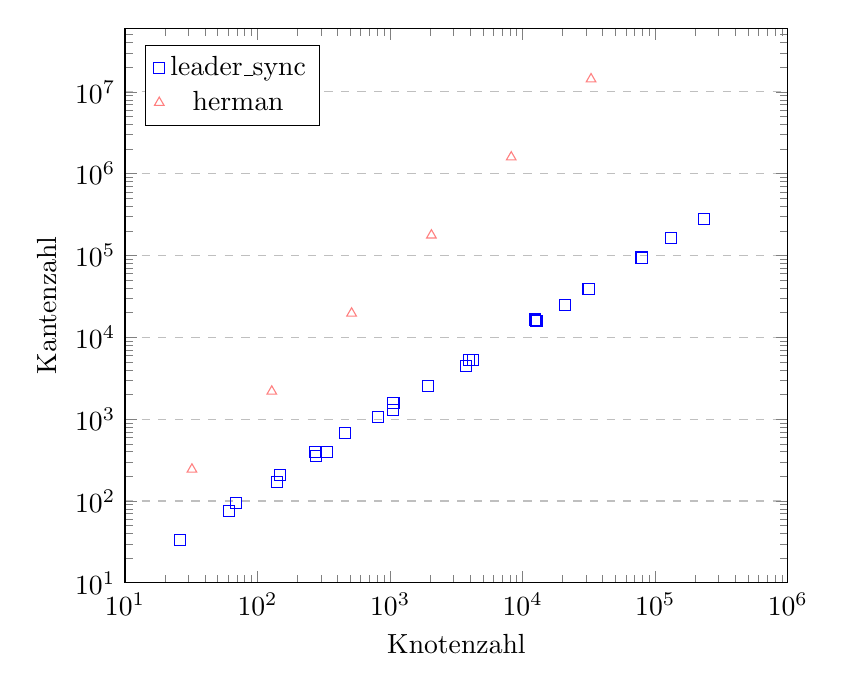
\begin{tikzpicture}
	\begin{axis}[
	xlabel={Knotenzahl},
	ylabel={Kantenzahl},
	xmin=10,
	xmax=1000000,
	xmode=log,
	ymin= 10,
	ymax=60000000,
	ymode=log,
	legend pos=north west,
	ymajorgrids=true,
	grid style=dashed,
	]
	\path[name path=axis] (axis cs:0,0) -- (axis cs:1,0);
	
	\addplot[only marks,color=blue,mark=square,name path=f]
	coordinates {
		(26,33)(69,95)(147,210)(273,397)(459,674)(1059,1570)(61,76)(274,354)(812,1067)(1933,2557)(3962,5257)(12400,16495)(141,172)(1050,1292)(4244,5267)(12709,15833)(31383,39158)(131521,164288)(335,398)(3759,4487)(20884,24979)(78784,94408)(234210,280865)
	};
	
	\addplot[only marks,color=red!50,mark=triangle,]
	coordinates {
		(8,28)(32,244)(128,2188)(512,19684)(2048,177148)(8192,1594324)(32768,14348908)
	};
	
	\addlegendentry{leader\_sync}
	\addlegendentry{herman}
	
	\end{axis}
	\end{tikzpicture}
\end{figure}


Abbildung \ref{fig-percentage} zeigt zunächst einmal, welchen Anteil das Lösen des linearen Gleichungssystems an der Gesamtzeit der Berechnung hat. Die Gesamtzeit umfasst alle Berechnungsschritte nach vollständigem Einlesen oder Generieren der \mc{} bis zum Ergebnis. Zur ihr zählen z.B. das Aufstellen der Matrix $P_{\rightarrow A}$ und das Berechnen der Gewichtsfunktion $S$ wie in Satz \ref{th-var} verwendet. Nicht inbegriffen ist das Einlesen von Dateien oder Generieren einer \mc{} für \textit{herman}. Wir sehen, dass sich für beide Beispiele unsere Erkenntnis aus den theoretischen Betrachtungen bestätigt, nämlich dass die Berechnungszeit im Wesentlichen vom Aufwand zum Lösen des linearen Gleichungssystems abhängt. Wäre dies nicht der Fall, so wäre zu überprüfen, ob die Implementierung hinsichtlich Effizienz im Speicherzugriff gröbere Fehler beinhaltet.

%=====================================================
% percentage les_time/total_time @ size_nodes

\begin{figure}
	\caption{Anteil Lösung des Gleichungssystem an Gesamtzeitaufwand}
	\label{fig-percentage}
	\centering
	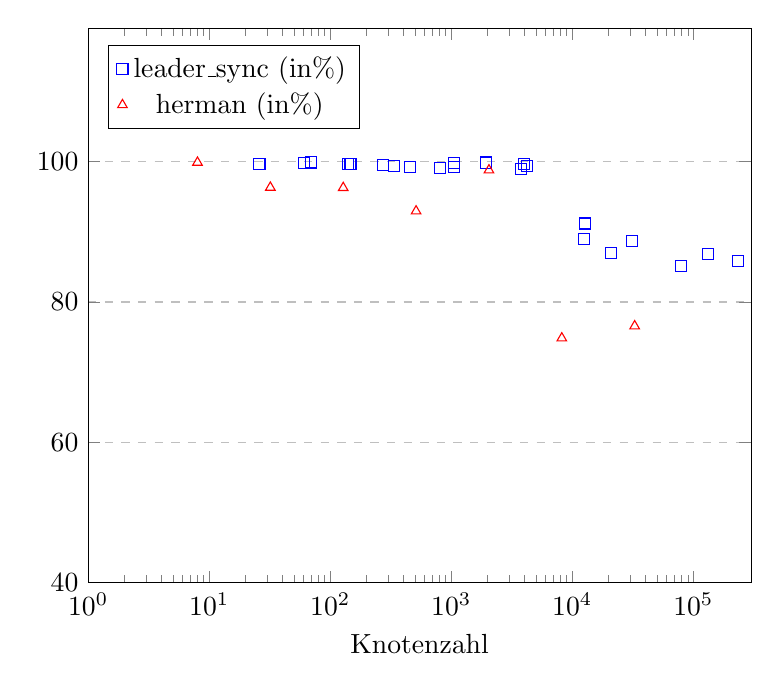
\begin{tikzpicture}
	\begin{axis}[
	xlabel={Knotenzahl},
	ylabel={},
	xmin=1,
	xmax=300000,
	xmode=log,
	ymin= 40,
	ymax=119,
	legend pos=north west,
	ymajorgrids=true,
	grid style=dashed,
	]
	\path[name path=axis] (axis cs:0,0) -- (axis cs:1,0);
	
	\addplot[only marks,color=blue,mark=square,name path=f]
	coordinates {
		(26,99.6873)(69,99.884)(147,99.6212)(273,99.5649)(459,99.2172)(1059,99.7976)(61,99.8605)(274,99.5487)(812,99.0917)(1933,99.8696)(3962,99.6054)(12400,88.9896)(141,99.6662)(1050,99.2031)(4244,99.3811)(12709,91.1847)(31383,88.7119)(131521,86.8379)(335,99.3776)(3759,98.8887)(20884,86.9314)(78784,85.1208)(234210,85.8437)
	};
	
	\addplot[only marks,color=red,mark=triangle,name path=f]
	coordinates {
		(8,99.8786)(32,96.3183)(128,96.2728)(512,92.9406)(2048,98.7838)(8192,74.852)(32768,76.5769)
	};
	
	\addlegendentry{leader\_sync (in\%)}
	\addlegendentry{herman (in\%)}
	\end{axis}
	\end{tikzpicture}
\end{figure}

% Kantenzahl in Abhängigkeit der Knotenzahl.

Nach diesen Vorbetrachtungen wollen wir nun den Zeitaufwand zur Lösung des linearen Gleichungssystems in Abhängigkeit von der Kantenzahl (Abbildung \ref{fig-in-edges1})  betrachten. Sofort erkennen wir, dass beide Messreihen keinen streng monotonen Verlauf aufweisen. Dies ist dadurch zu erklären, dass AMGCL bei gewissen Größen der \mc{} beginnt, jeweils weitere Matrizen in der Hierarchie des Mehrgitterverfahrens aufzustellen. Wir sehen für \textit{leader\_sync} drei maximale Intervalle mit (bis auf Ausreißer in der Messung) monoton steigenden Messwerten. Entsprechend wurden keine, genau eine, beziehungsweise genau zwei zusätzliche Matrizen aufgestellt. Diese Zuordnung lässt sich eindeutig beobachten, wenn man die Log-Ausgaben von AMGCL betrachtet. Analog wird für \textit{herman} ab $N=13$ eine zweite, gröbere Matrix aufgestellt. Betrachten wir die Messwerte für größere Kantenzahlen, so lässt sich ablesen, dass der Zeitaufwand in etwa linear von der Kantenzahl abhängt. Schlüsse auf den Verlauf des Graphen für noch größere Eingaben erscheinen auf Basis der Messwerte nicht begründbar und möchten wir hier nicht vornehmen.

Betrachtet haben wir hier bewusst nur die Zeit für den Schritt des Lösens der zwei Gleichungssysteme, nicht jedoch die Gesamtzeit. Man könnte diese Punkte mithilfe von Abbildung \ref{fig-percentage} einzeichnen und würde dann nahezu identische Punkte zu den bereits eingezeichneten erhalten. Insbesondere deswegen wollen wir hier darauf verzichten.

% time_solve_linear_system @ size_edges

\begin{figure}
	\caption{Zeitaufwand in Abhängigkeit der Kantenzahl}
	\label{fig-in-edges1}
	\centering
	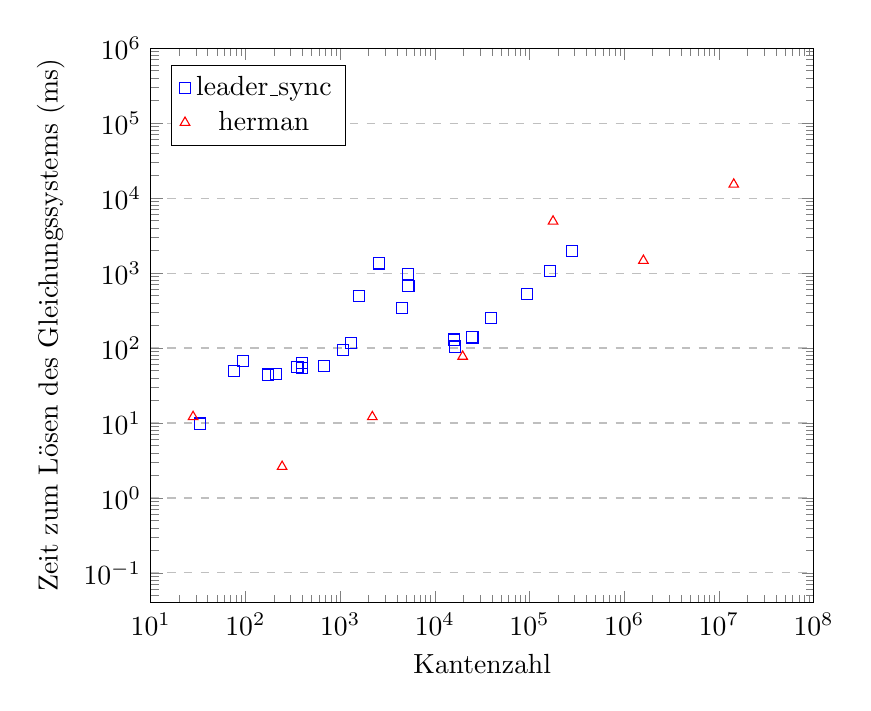
\begin{tikzpicture}
	\begin{axis}[
	xlabel={Kantenzahl},
	ylabel={Zeit zum Lösen des Gleichungssystems (ms) },
	xmin=10,
	xmax=100000000,
	xmode=log,
	ymode=log,
	ymin= 0.04,
	ymax=1000000,
	legend pos=north west,
	ymajorgrids=true,
	grid style=dashed,
	]
	\path[name path=axis] (axis cs:0,0) -- (axis cs:1,0);
	
	\addplot[ only marks,color=blue,mark=square,name path=f]
	coordinates {
		(33,9.82)(95,66.3707)(210,44.7318)(397,63.0215)(674,58.1665)(1570,495.6469)(76,49.9831)(354,55.259699999999995)(1067,94.4225)(2557,1343.5230000000001)(5257,975.068)(16495,104.6482)(172,44.3029)(1292,116.6879)(5267,669.7491)(15833,129.73489999999998)(39158,251.1644)(164288,1058.4239)(398,53.6763)(4487,340.5793)(24979,138.3345)(94408,524.8805)(280865,1971.8429999999998)
	};
	
	\addplot[only marks,color=red,mark=triangle,name path=f]
	coordinates {
		(28,12.0933)(244,2.6161000000000003)(2188,12.0549)(19684,77.05510000000001)(177148,4900.8295)(1594324,1465.4203)(14348908,15232.2595)
	};
	
	\addlegendentry{leader\_sync}
	\addlegendentry{herman}
	\end{axis}
	\end{tikzpicture}
\end{figure}

Um noch einen Vergleich anstellen zu können, wurde die verwendete C++ Bibliothek zum Lösen des Gleichungssystems AMGCL einmal durch die Bibliothek Eigen ausgetauscht. Speziell wurde der Algorithmus \textit{BiCGSTAB}, der von Eigen implementiert wird, genutzt, um die Gleichungssysteme mit dünn besetzten Matrizen zu lösen. BiCGSTAB ist dafür bekannt sehr schnell zu laufen, allerdings auch Rundungsfehler bei den Ergebnissen zu produzieren, weswegen er in der Praxis nicht häufig verwendet wird. Dieses Phänomen konnte bei der Entwicklung auch beobachtet werden. Da Eigen selbst Datenstrukturen für die Speicherung von Matrizen mitbringt, welche verwendet werden müssen, um den Algorithmus anzuwenden, und diese entsprechend anders zu initialisieren sind, bietet es sich an, einfach die Gesamtzeit (ohne Einlesen von Dateien) zu messen, welche zur Ermittlung der Varianzen gebraucht wird. Abbildung \ref{eigen} zeigt die Messreihen der Gesamtzeit für \textit{herman} und \textit{leader\_sync}, wobei die Verwendung von Eigen und AMGCL gegenüber gestellt wird. Wie wir sehen, verhält sich der Zeitaufwand bei der Variante Eigen in etwa linear zur Kantenzahl. Sogar bietet diese Variante kürzere Berechnungszeiten für kleinere Modelle.

\begin{figure}
	\caption{Zeitaufwand in Abhängigkeit der Kantenzahl}
	\label{eigen}
	\centering
	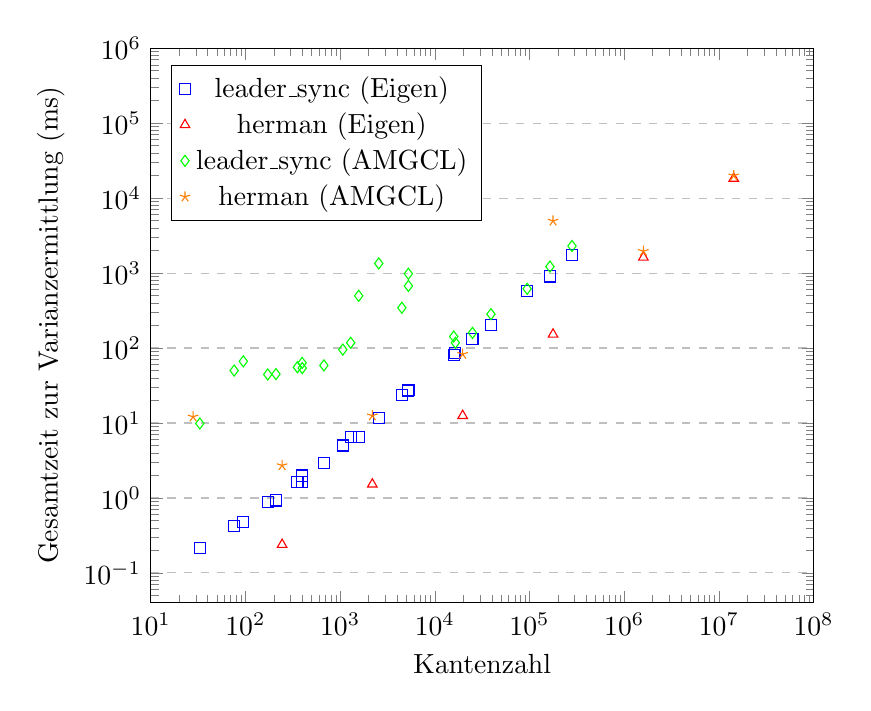
\begin{tikzpicture}
	\begin{axis}[
	xlabel={Kantenzahl},
	ylabel={Gesamtzeit zur Varianzermittlung (ms) },
	xmin=10,
	xmax=100000000,
	xmode=log,
	ymode=log,
	ymin= 0.04,
	ymax=1000000,
	legend pos=north west,
	ymajorgrids=true,
	grid style=dashed,
	]
	\path[name path=axis] (axis cs:0,0) -- (axis cs:1,0);
	
	\addplot[ only marks,color=blue,mark=square,name path=f]
	coordinates {
		(33,0.2169)(95,0.4725)(210,0.9264)(397,1.6495)(674,2.9137)(1570,6.4779)(76,0.4179)(354,1.6347)(1067,5.0114)(2557,11.7838)(5257,27.0573)(16495,86.6749)(172,0.8896)(1292,6.4475)(5267,27.8474)(15833,79.8205)(39158,203.4906)(164288,902.0273)(398,1.9912)(4487,23.3781)(24979,132.2275)(94408,570.7666)(280865,1755.6267)
	};
	
	\addplot[only marks,color=red,mark=triangle,name path=f]
	coordinates {
		(28,0.0226)(244,0.2386)(2188,1.5244)(19684,12.5113)(177148,152.4009)(1594324,1617.6304)(14348908,18259.9604)
	};

	\addplot[ only marks,color=green,mark=diamond,name path=f]
	coordinates {
		(33,9.8508)(95,66.4478)(210,44.9019)(397,63.2969)(674,58.6254)(1570,496.6521)(76,50.0529)(354,55.5102)(1067,95.288)(2557,1345.2771)(5257,978.931)(16495,117.596)(172,44.4513)(1292,117.6252)(5267,673.9199)(15833,142.2771)(39158,283.1237)(164288,1218.8505)(398,54.0125)(4487,344.4068)(24979,159.1307)(94408,616.63)(280865,2297.0147)
	};
	
	\addplot[only marks,color=orange,mark=star,name path=f]
	coordinates {
		(28,12.108)(244,2.7161)(2188,12.5216)(19684,82.9079)(177148,4961.1665)(1594324,1957.7559)(14348908,19891.462)
	};
	
	\addlegendentry{leader\_sync (Eigen)}
	\addlegendentry{herman (Eigen)}
	
	\addlegendentry{leader\_sync (AMGCL)}
	\addlegendentry{herman (AMGCL)}
	\end{axis}
	\end{tikzpicture}
\end{figure}

Zumindest im Rahmen der Aussagekraft unserer Messdaten lässt sich zusammenfassend erkennen, dass die Zahl der Kanten kennzeichnend für die benötigte Rechenzeit ist und dass letztere sich in etwa linear zur Zahl der Kanten verhält.

\subsection{Grenzen der Aussagekraft}

Wie bereits kurz zur Erläuterung der Abbildungen erwähnt, steigt der Bedarf an Arbeitsspeicher natürlich recht schnell an, wenn \mc{}n eines bestimmten Modells betrachtet werden und die Zahl der Kanten in Abhängigkeit der Parameter des Modells exponentiell wächst. Bei Speicherung der Matrizen mittels HashMaps wie im Fall von \textit{MC Analyzer} ist davon auszugehen, dass sich der Speicherbedarf linear zur Zahl der Kanten verhält.
Bei Rechenzeiten unter $100\mathrm{s}$ ist hier nicht die Zeit und damit die Taktfrequenz des Prozessors die limitierende Ressource, sondern vielmehr der zur Verfügung stehende Arbeitsspeicher. Ausgaben des Debuggers und Logs von AMGCL zu Folge ist der für das Lösen des linearen Gleichungssystems benötigte RAM nach Aufstellen der Eingabematrix im Vergleich zu dieser Matrix bei den gemessenen Beispielen verschwindend gering. Es genügt nach diesen Beobachtungen im Wesentlichen zu schauen, wie viel Platz zur Darstellung der \mc{} im Speicher benötigt wird. Es wäre weiterführend interessant, sich Mittel und Methoden zu überlegen und zu implementieren, den tatsächlichen Speicherbedarf zu messen und in Abhängigkeit von der Zahl der Kanten darzustellen.

Wir haben bei den Messungen gesehen, dass AMGCL bis zu drei Matrizen im Mehrgitterverfahren verwendet. Ob sich die lineare Abhängigkeit der Rechenzeit von der Zahl der Kanten auch bei noch größeren \mc{}n und den mit diesen verbundenen Matrizen fortsetzt, lässt sich an dieser Stelle schwer einschätzen. Auch wäre es interessant zu analysieren, wie es sich bei derart größeren \mc{}n verhält, bei welchen dann entsprechend mehr Matrizen in der Mehrgitterhierarchie berechnet werden. 

Zur Speicherung der Matrizen wurden Hashtabellen genutzt, wie es auch in der Dokumentation von AMGCL vorgeschlagen wird. Die Art und Weise der Speicherung und der damit verbundene Zugriff beeinflusst wesentlich die Laufzeit eines darauf operierenden Algorithmus'. Für weiterführenden Untersuchungen wäre es interessant herauszufinden, welche besseren Möglichkeiten es zur Speicherung möglicherweise gibt. Es wäre insbesondere interessant zu prüfen, ob das von der Bibliothek Eigen mitgebrachte Datenformat zur Speicherung von dünnbesetzten Matrizen auch mit AMGCL verwendet werden kann. Die Speicherung der eingelesenen \mc{} selbst müsste dazu angepasst werden, um nicht den erhöhten Zeitaufwand bei der Initialisierung in Kauf nehmen zu müssen. Mit Optimierungen könnte das Problem jedoch auch nicht unter linearer Zeit gelöst werden, da zum vollständigen Lesen der \mc{} mindestens über die Kanten iteriert werden muss.


\section{Ein Blick auf MDPs}

Markow-Entscheidungsprozesse (\textit{Markov-Decision-Processes, MDPs}) können als Erweiterung bzw. Verallgemeinerung von \mc{}n angesehen werden. Wir möchten daher in diesem Abschnitt einen kurzen Blick auf MDPs werfen, das Problem minimaler Varianzen adressieren und einen Ansatz zu dessen Lösung diskutieren.

\subsection{Was sind MDPs?}
\newcommand{\mdpex}{$M = (Q,A,P,I)$}
\newcommand{\mdp}{Mar\-kow-Ent\-schei\-dungs\-pro\-zess}
\newcommand{\mact}{\mathrm{Act}}
\begin{definition}\label{def-mdp}
	Ein Tupel \mdpex{} nennen wir \mdp{}, wenn es folgende Eigenschaften erfüllt:
	\begin{enumerate}[(a)]
		\item $Q$ ist eine endliche Menge, d.h. $|Q|<\infty$.
		\item $A$ ist eine endliche Menge, genannt die Menge der Aktionen: $|A| < \infty$.
		\item $P$ ist eine Funktion $Q \times A \times Q \to [0,1]$ mit
		\begin{equation}
		\forall q\in Q, \alpha\in A : \sum_{q' \in Q}{P(q,\alpha,q')} \in \{0,1\}
		\end{equation}
		und beschreibt die Wahrscheinlichkeiten der Zustandsübergänge.
		\item $I$ ist eine Funktion $Q \to [0,1]$ mit $\sum_{q \in Q}{I(q)} = 1$ und beschreibt die initiale Verteilung.
		\item In jedem Zustand ist mindestens eine Aktion verfügbar:
		\begin{equation}
			\forall q\in Q : 0 < | \mathrm{Act}(q) | < \infty
		\end{equation}
		Dabei bezeichnen wir für $q \in Q$ mit $\mathrm{Act}(q) \coloneqq \{\alpha \in A \mid \exists q' \in Q : P(q,\alpha,q') > 0\}$ die Menge der Aktionen, für die eine Wahrscheinlichkeitsverteilung für Folgezustände existiert. \label{item-b-270820}
	\end{enumerate}
\end{definition}	
Die Semantik eines MDP ist so zu verstehen, dass von einem Zustand $q \in Q$ aus zunächst eine Aktion $\alpha \in \mathrm{Act}(q)$ gewählt werden muss. Danach erfolgt ein probabilistischer Zustandsübergang wie in einer \mc{}, definiert durch $q' \mapsto P(q,\alpha,q')$. Die initiale Verteilung $I$ ordnet jedem Zustand wie bei \mc{}n die Wahrscheinlichkeit zu, dass ein Lauf in diesem Zustand startet.
Das Auswählen einer Aktion in jedem Zustand kann durch einen sogenannten Scheduler beschrieben werden:
\newcommand{\msch}{\mathrm{Schedulers}}
\begin{definition}
	Sei \mdpex{} ein \mdp{}. Ein Scheduler für $M$ ist eine Funktion $\mathcal{S} : Q^+ \to A$ mit der Eigenschaft
	\begin{equation}
	\forall n \in \mathbb{N}_{>0}, \pi \in Q^n\ : \mathcal{S}(\pi) \in \mathrm{Act}(\pi_{n-1})\text{.}
	\end{equation}
	Dabei beschreibt $\pi_{n-1}$ den letzten Eintrag des Tupels $\pi$. Mit $Q^+$ bezeichnen wir die Menge aller nichtleeren Tupel von Elementen aus $Q$, also $Q^+ \coloneqq \bigcup_{n \in \mathbb{N}_{>0}} Q^n$. In Worten sagt die Bedingung, der Scheduler darf immer nur eine Aktion wählen, für welche Zustandsübergänge vom Zustand $\pi_{n-1}$ existieren. Der Scheduler ordnet jedem Pfadpräfix die zu wählende Aktion zu und löst auf diese Weise den Nichtdeterminismus eines \mdp{}es auf.
	Wir bezeichnen die Menge aller Scheduler für $M$ mit $\mathrm{Schedulers}(M)$.
\end{definition}

\!Offenbar ergibt sich aus einem MDP \mdpex{} und einem Scheduler $\mathcal{S} : Q^+ \to A$ für $M$ eine eindeutig bestimmte \mc{}, bezeichnet durch $M_{\mathcal{S}}$, indem die Aktionen gemäß des Schedulers gewählt werden. Eine recht offensichtliche Konstruktion von $M_{\mathcal{S}}$ ist in \cite{Bai08} beschrieben. Ziel dieses Abschnittes soll es sein, uns der folgenden Problemstellung zu widmen:

\medskip
{ \slshape
	Gegeben sei ein \mdp{} \mdpex{}, eine Menge $T \subseteq Q$ von Zielzuständen und eine Gewichtsfunktion $R : Q \times A \times Q \to \mathbb{R}_{\geq 0}$ mit der Eigenschaft, dass unter jedem Scheduler für $M$ in der resultierenden \mc{} mit sicherer Wahrscheinlichkeit ein Zustand aus $T$ nach endlich vielen Schritten erreicht wird.
	
	Gesucht ist ein Scheduler $\mathcal{S}$ mit möglichst kleiner Varianz akkumulierter Kantengewichte in der resultierenden \mc{} $M_{\mathcal{S}}$. Gibt es für jeden MDP einen Scheduler mit minimaler Varianz oder existiert ein MDP mit einem Infimum der Varianz, wobei kein Scheduler das Infimum erreicht? Wie berechnen wir
	\[\inf_{\mathcal{S} \in \mathrm{Schedulers}(M)}{\mvar(M_\mathcal{S})} \text{\slshape ?}\]
}
\medskip

\subsection{Resultierende \mc{}n}

Die Problemstellung möchten wir in erster Linie als Motivation verstehen. Wir werden die Fragen nicht abschließend beantworten, jedoch möchten wir einen Ansatz präsentieren und begründen, wie zum Finden von Schedulern, welche eine kleine Varianz aufweisen, vorgegangen werden kann.
Dazu beginnen wir, die bereits genannte resultierende \mc{} $M_{\mathcal{S}}$ formal zu präzisieren. Jedoch werden wir eine andere Konstruktion verwenden als Baier und Katoen \cite{Bai08}. Zunächst möchten wir eine dafür nützliche Schreibweise einführen:
\begin{definition}
	Seien \mdpex{} ein MDP, $S\in \msch(M)$ ein Scheduler für $M$ und $q\in Q$ ein beliebiger Zustand von $M$. Dann definieren wir:
	\begin{equation}
		S_{\leftarrow q} : Q^+ \to A : (p_0,\dots,p_{n-1}) \mapsto S(q,p_0,\dots,p_{n-1})
	\end{equation}
	$S_{\leftarrow q}$ ist offensichtlich wieder ein Scheduler für $M$: $S_{\leftarrow q} \in \msch(M)$
\end{definition}

\newcommand{\gmc}{generische \mc{}}
Wir beschreiben nun eine rudimentäre Art \mc{}, die wir \gmc{} nennen wollen.
\begin{definition}
	Eine Tupel $G=(Q,P)$ heißt \gmc{}, wenn eine \mc{} $M$ mit \mcex{} existiert. Eine \gmc{} ist so gesehen eine \mc{} abzüglich der initialen Verteilung.
\end{definition}

Wir wollen diese Definition nun nutzen, um jedem MDP $M$ eine \gmc{} zuzuordnen, welche durch Hinzufügen einer jeweils geeigneten initialen Verteilung zur resultierenden \mc{} $M_\mathcal{S}$ für einen beliebigen Scheduler $S \in \msch(M)$ komplettiert werden kann.

\newcommand{\mgen}{\mathrm{Gen}}
\begin{definition}
	Sei \mdpex{} ein MDP. Mit
	\begin{equation}
		\mgen(M):= (\mathrm{Schedulers}(M)\times Q,\tilde{P})
	\end{equation}
	bezeichnen wir die \gmc{} zu $M$. Dabei sei $\tilde{P}$ definiert als:
	\begin{align}
		\tilde{P} &: (\mathrm{Schedulers}(M)\times Q) \times (\mathrm{Schedulers}(M)\times Q) \to [0,1]\text{ , mit} \nonumber \\
		&\big((\mathcal{S}_1,q),(\mathcal{S}_2,q')\big) \mapsto \begin{cases}
		P(q,\alpha,q') & \text{falls } \mathcal{S}_2 = (\mathcal{S}_1)_{\leftarrow q}, \alpha = \mathcal{S}_1(q)\\
		0 & \text{sonst}
		\end{cases}
	\end{align}
\end{definition}

Die \gmc{} $\mgen(M)$ ist wohldefiniert, denn $\mathcal{S}_1(q) \in \mact(q)$. Da $\mact(q)$ mindestens eine Aktion beinhaltet, gibt es für jeden Zustand der generischen \mc{} eine Menge ausgehender Kanten, deren Wahrscheinlichkeiten sich aufgrund der Bedingungen aus Definition \ref{def-mdp} zu $1$ aufsummieren. 

Für einen MDP \mdpex{} und einen Scheduler $\mathcal{S}\in \msch(M)$ lässt sich die resultierende \mc{} nun auffassen als $M_\mathcal{S} := (Q',P',I')$ mit $(Q',P') = \mgen(M)$ und
\begin{equation}
	I'(\mathcal{S}',q) := \begin{cases}
		I(q) & \text{falls }\mathcal{S}'=\mathcal{S}\\
		0 & \text{sonst}
	\end{cases}\text{.}
\end{equation}
Obgleich diese \mc{} in vielen Fällen zahlreiche unerreichbare Zustände mit sich bringt, welche für z.B. die Betrachtung von \var{}en irrelevant sind, erhalten wir zu einer Familie von Schedulern stets eine Familie von \mc{}en, die sich höchstens in der initialen Verteilung unterscheiden.

Wir wollen nichtnegative Kantengewichte auf \mdp{}en analog zu Kantengewichten auf \mc{}n betrachten. Solche Kantengewichte beschreiben wir durch eine Funktion
\begin{equation}
R : Q \times A \times Q \to \mathbb{R}_{\geq 0}\text{.}
\end{equation}
Wenn von Zustand $q\in Q$ mit Wahl von Aktion $\alpha\in A$ in Zustand $q'\in Q$ übergegangen wird, so wird das Gewicht $R(q,\alpha,q')$ aufgesammelt. 
Wir wollen kurz darauf eingehen, wie die Kantengewichte in der resultierenden \mc{} aussehen: Für einen MDP \mdpex{} und $\mathcal{S} \in \msch(M)$ sowie $q,q' \in Q$ ergibt sich für die Gewichtsfunktion $\tilde{R}$ der resultierenden \mc{}
\begin{equation}
	\tilde{R}\big((\mathcal{S},q), (\mathcal{S}_{\leftarrow q},q')\big) = R(q,\mathcal{S}(q),q') \text{.}
\end{equation}


Während beispielsweise maximale Wahrscheinlichkeiten zum Erreichen einer Zielmenge stets durch einen sogenannten memoryless Scheduler erreicht werden können \cite{Bai08}, d.h. einen Scheduler, der in einem Zustand unabhängig von dem vorangegangenen Pfadpräfix immer dieselbe Aktion wählt, stellen wir zunächst fest, dass diese Art von Scheduler für unser Problem nicht ausreichend ist. Dies können wir anhand eines einfachen Beispiels zeigen:

\begin{beispiel}
	\label{ex-meml-sched}
	Wir verwenden hier eine Notation analog zu den Darstellungen für \mc{}n, siehe Beispiel \ref{example-mc}. Kanten werden in der Form $\alpha : p : r$ beschriftet, wobei eine solche Kante von $q_1$ nach $q_2$ bedeutet, dass $\alpha \in \mathrm{Act}(q_1)$, $P(q_1,\alpha,q_2) = p$ und $R(q_1,\alpha,q_2) = r$ gilt:
\begin{center}
	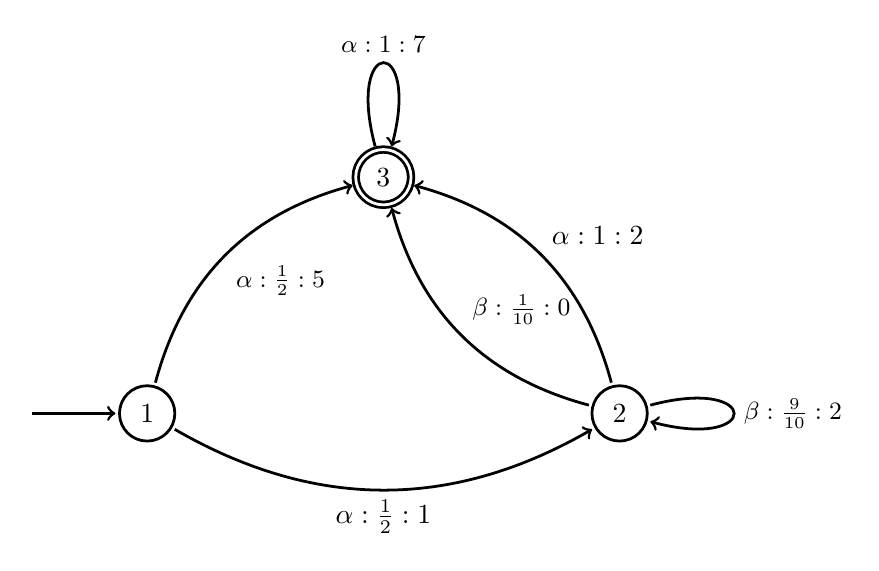
\begin{tikzpicture}[auto,swap,scale=3]
	
	% First we draw the vertices
	\foreach \pos/\name in {{(0,0)/1}, {(2,0)/2}}
	\node[vertex] (\name) at \pos {$\name$};
	
	% First we draw the vertices
	\foreach \pos/\name in {{(1,1)/3}}
	\node[target] (\name) at \pos {$\name$};
	
	% Connect vertices with edges and draw weights
	\foreach \source/ \dest /\weight in {
		1/3/{\alpha:\frac{1}{2}:5},
		2/3/{\beta:\frac{1}{10}:0}
	}
	\path[edge] (\source) to[bend left] node[weight]{$\weight$} (\dest);
	
	% Connect vertices with edges and draw weights
	\foreach \source/ \dest /\weight in {
		2/3/{\alpha:1:2},
		1/2/{\alpha:\frac{1}{2}:1}
	}
	\path[edge] (\source) to[bend right] node{$\weight$} (\dest);
	
	% Connect vertices with edges and draw weights
	%\foreach \source/ \dest /\weight in {
	%}
	%\path[edge] (\source) to node[weight]{$\weight$} (\dest);
	
	\foreach \source/ \dest /\weight in {
		2/2/{\beta:\frac{9}{10}:2}
	}
	\path[edge] (\source) to[loop right] node[weight]{$\weight$} (\dest);

	\foreach \source/ \dest /\weight in {
	3/3/{\alpha:1:7}
	}
	\path[edge] (\source) to[loop above] node[weight]{$\weight$} (\dest);
	
	% Draw initial state
	\path[edge] (-0.5,0) to (1);
	
	\end{tikzpicture}
\end{center}
\end{beispiel}

Für Beispiel \ref{ex-meml-sched} gibt es genau zwei memoryless Scheduler, da nur die Wahl zwischen $\alpha$ und $\beta$ im Zustand $2$ besteht:
\begin{itemize}
	\item Wählen wir $\alpha$, so ergibt sich als Erwartungswert in der resultierenden \mc{} $\mexp(R) = 4$ und als \var{} $\mvar(R) = 1$ bei genau zwei möglichen Pfaden mit einer Wahrscheinlichkeit von je $\frac{1}{2}$.
	\item Wählen wir jedoch $\beta$, so ergibt sich nach $\mexp_{2}(R) = \frac{9}{10} \cdot (\mexp_{2}(R) + 2) + \frac{1}{10} \cdot 0$ schließlich $\mexp_{2}(R) = 18$ und $\mexp_{1}(R) = 12$. Analog zu unseren Betrachtungen aus vorangegangenen Abschnitten, bezeichnen wir den Erwartungswert aufsummierter Gewichte aus der Funktion $R$ für den Start in Knoten $i$ mit $\mexp_i(R)$. Die Varianz in diesem Fall ergibt sich zu $\mvar(R) = \frac{1}{2} \cdot (12 - 5)^2 + \dots \geq \frac{49}{2}$ und wir betrachten diesen Scheduler nicht weiter, da wir bereits zuvor einen besseren (bzgl. Minimierung der \var{}) gesehen haben.
\end{itemize}
Betrachten wir nun einen Scheduler, der nicht zur Klasse der memoryless Scheduler gehört: Wählen wir beim ersten Besuch von Zustand $2$ die Aktion $\beta$ und beim zweiten Besuch von Zustand $2$, sofern er denn eintritt, die Aktion $\alpha$, so erhalten wir eine \mc{} äquivalent zur folgenden Abbildung und mit den resultierenden Kenngrößen $\mexp(R) = 4,8$ und $\mvar(R) = 0,76$.
\begin{center}
	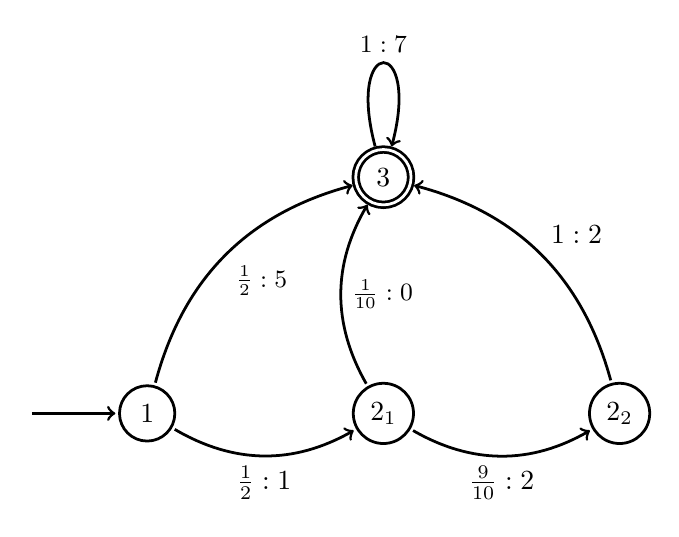
\begin{tikzpicture}[auto,swap,scale=3]
	
	% First we draw the vertices
	\foreach \pos/\name in {{(0,0)/1}, {(1,0)/2_1}, {(2,0)/2_2}}
	\node[vertex] (\name) at \pos {$\name$};
	
	% First we draw the vertices
	\foreach \pos/\name in {{(1,1)/3}}
	\node[target] (\name) at \pos {$\name$};
	
	% Connect vertices with edges and draw weights
	\foreach \source/ \dest /\weight in {
		1/3/{\frac{1}{2}:5},
		2_1/3/{\frac{1}{10}:0}
	}
	\path[edge] (\source) to[bend left] node[weight]{$\weight$} (\dest);
	
	% Connect vertices with edges and draw weights
	\foreach \source/ \dest /\weight in {
		2_2/3/{1:2},
		1/2_1/{\frac{1}{2}:1},
		2_1/2_2/{\frac{9}{10}:2}
	}
	\path[edge] (\source) to[bend right] node{$\weight$} (\dest);
	
	% Connect vertices with edges and draw weights
	%\foreach \source/ \dest /\weight in {
	%}
	%\path[edge] (\source) to node[weight]{$\weight$} (\dest);
	
	\foreach \source/ \dest /\weight in {
	3/3/{1:7}
	}
	\path[edge] (\source) to[loop above] node[weight]{$\weight$} (\dest);
	
	% Draw initial state
	\path[edge] (-0.5,0) to (1);
	
	\end{tikzpicture}
\end{center}

Wir haben in der Abbildung bewusst nicht explizit unsere Definition einer resultierenden \mc{} aus einem MDP und einem Scheduler angewandt, sondern unerreichbare Zustände sofort außen vor gelassen. Mit diesem Beispiel haben wir gezeigt, dass die Klasse der memoryless Scheduler im Allgemeinen nicht zu minimalen Varianzen führt. Gleichzeitig wollen wir noch einmal darauf hinweisen, dass an dieser Stelle noch nicht geklärt ist, ob tatsächlich für jeden MDP ein Scheduler mit minimaler Varianz existiert oder ob nur eine Folge von Schedulern existieren muss, sodass der Grenzwert der Varianzen gegen das Infimum der Varianzen aller Scheduler konvergiert.

\subsection{Ein Ansatz zum Minimieren von Varianzen}

Als Intuition aus Beispiel \ref{ex-meml-sched} können wir uns überlegen: Nehmen wir einmal an, wir kennen den Erwartungswert, zu welchem ein Scheduler mit minimaler oder zumindest möglichst kleiner (nah am Infimum) Varianz existiert. Dann können wir versuchen, den Scheduler so zu konstruieren, dass wir auf jedem Pfad die Summe der Kantengewichte möglichst nah an den bekannten \expect{} bringen. Wir wollen aus dieser Intuition einen Ansatz entwickeln, um Scheduler mit minimalen oder zumindest ziemlich kleinen \var{}en zu ermitteln.

Wir definierten bereits die Varianz für \mc{}n. Wir können nun die Varianz akkumulierter Kantengewichte bis zum Erreichen einer Zielzustandsmenge $T$ in einem MDP \mdpex{} in Abhängigkeit der Gewichtsfunktion $R$ und des Schedulers $\mathcal{S}$ schreiben als
\[
\mvar^{\mathcal{S}}(R) = \sum_{q \in Q}{I(q)} \cdot \sum_{\pi \in \pfin_{(\mathcal{S},q) \rightarrow (\msch(M)\times T)}(\mgen(M))}{\tilde{P}(\pi) \cdot (\tilde{R}(\pi) - \mu^{\mathcal{S}})^2}\text{,}
\]
wenn $\mgen(M)=(\msch(M)\times Q, \tilde{P})$ und $\tilde{R}$ die entsprechende Gewichtsfunktion auf der resultierenden \mc{} ist.
Dies entspricht unserer bisherigen Definition von \var{} und bezieht stets den Erwartungswert
\[
\mu^{\mathcal{S}} = \sum_{q \in Q}{I(q)} \cdot \sum_{\pi \in \pfin_{(\mathcal{S},q) \rightarrow (\msch(M)\times T)}(\mgen(M))}{\tilde{P}(\pi) \cdot \tilde{R}(\pi)}
\]
ein. Wir nutzen jeweils wieder die übliche Fortsetzung von Wahrscheinlichkeiten bzw. Kantengewichten auf Pfade. Nun wollen wir einen im Vergleich zur \var{} allgemeineren Begriff einführen:
\newcommand{\vt}{Target-Varianz}
\newcommand{\mvt}{\mathcal{V}\!ar \mathcal{T}\!\!ar}
\newcommand{\vtex}{$\mvt(M_{\mathcal{S}},x)$}
\begin{definition}[\vt]\label{def-vt}
		Seien \probspaceex{} ein \probspace{}, $X$ eine \rvar{} auf \probspaceex{} und $t \in \mathbb{R}$. Mit
	\begin{equation}
	\mvt_{\probspaceexraw{}}(X,t) \coloneqq \mathcal{E}_{\probspaceexraw{}}\left(\left(X - t\right)^{2}\right)
	\end{equation}
	bezeichnen wir die \vt{} von $X$ zum Ziel $t$ auf  \probspaceex{}. Sollte der Kontext \probspaceex{} klar sein, schreiben wir kurz $\mvt(X,t)$.
	

\end{definition}

Demnach betrachten wir nun die nach Wahrscheinlichkeiten gewichtete mittlere quadratische Abweichung zu einem frei gewählten Zielwert (\textit{engl. target}) $t$ statt zum \expect{}. Offenbar ist die \var{} ein Spezialfall der \vt{}, da $\mvt_{\probspaceexraw{}}(X,\mu) = \mvar_{\probspaceexraw{}}(X)$, wenn $\mu = \mathcal{E}_{\probspaceexraw{}}(X)$ der Erwartungswert ist. Weiterhin stellen wir fest, dass sich die \vt{} als quadratische Funktion auffassen lässt:


\begin{lemma}\label{lem-vtqf}
	Sei \probspaceex{} ein \probspace{}, $X$ eine \rvar{} auf \probspaceex{} und $t \in \mathbb{R}$. Dann gilt:
	\begin{equation}
	\mvt(X,t) = \left(t - \mathcal{E}(X)\right)^2 + \mvar(X)
	\end{equation}
\end{lemma}
\begin{beweis}
	\begin{align*}
	\mvt(X,t) & =  \sum_{\omega \in \Omega}{P(\omega) \cdot \left((X(\omega)-t)^2\right)} \\
	%\implies & & f(t) & = \sum_{\omega \in \Omega}{P(\omega) \cdot \left(t^2 -2tX(\omega) + \left(X(\omega)\right)^2\right)} \\
	 & = \sum_{\omega \in \Omega}{P(\omega) \cdot \left(t^2 -2tX(\omega) + \left(\mathcal{E}(X)\right)^2 - \left(\mathcal{E}(X)\right)^2 + \left(X(\omega)\right)^2\right)} \\
	 & = \left(t - \mathcal{E}(X)\right)^2 - \left(\mathcal{E}(X)\right)^2 + \mathcal{E}(X^2) \\
	 & = \left(t - \mathcal{E}(X)\right)^2 + \mvar(X) \\
	\end{align*}
\end{beweis}
Insbesondere sehen wir als unmittelbare Konsequenz von Lemma \ref{lem-vtqf}, dass die \vt{} nie kleiner sein kann als die \var{}:
\begin{korollar}\label{kor-vtt-rel}
	Sei \probspaceex{} ein \probspace{}, $X$ eine \rvar{} auf \probspaceex{} und $t \in \mathbb{R}$. Dann gilt:
	\begin{equation}
		\mvt(X,t) \geq \mvar(X)
	\end{equation}
\end{korollar}
\begin{comment}
\begin{beweis}
Sei $\mu = \mathcal{E}_{\probspaceexraw{}}(X)$ der Erwartungswert von $X$. So erhalten wir:
\begin{align*}
& & (t-\mu)^2 &\geq 0\\
\implies & & -2t\mu + 2\mu^2 + t^2 - \mu^2 &\geq 0\\
\implies & & \sum_{\omega \in \Omega}{P(\omega)} \cdot (-2t X(\omega) + 2\mu X(\omega) + t^2 - \mu^2) &\geq 0\\
\implies & & \sum_{\omega \in \Omega}{P(\omega)} \cdot \left((X(\omega)-t)^2 - (X(\omega) - \mu)^2\right) &\geq 0\\
\implies & & \sum_{\omega \in \Omega}{P(\omega)} \cdot \left((X(\omega)-t)^2\right) &\geq \sum_{\omega \in \Omega}{P(\omega)} \cdot \left((X(\omega) - \mu)^2\right)\\
\end{align*}
\end{beweis}
\end{comment}


Wir haben nun gesehen, dass die Funktion
\[
f : \mathbb{R} \to \mathbb{R} : t \mapsto \mvt(X,t)
\]
als quadratische Funktion der Form $f(t) = (t-a)^2 + b$ mit $a,b \in \mathbb{R}$ aufgefasst werden kann, wenn der diskrete Wahrscheinlichkeitsraum und $X$ als konstant angesehen werden.  Dies werden wir uns zu Nutze machen, um gezielt nach den \expect{}en zu suchen, für welche ein Scheduler zu einem MDP existiert, der eine \mc{} mit genau diesem \expect{} erzeugt und deren \var{} möglichst klein oder sogar minimal ist.
\begin{comment}
Dabei ergibt sich $a = \mathcal{E}(X)$ und $b = \mvar(X)$:
\begin{align*}
	& & f(t) & =  \sum_{\omega \in \Omega}{P(\omega) \cdot \left((X(\omega)-t)^2\right)} \\
	%\implies & & f(t) & = \sum_{\omega \in \Omega}{P(\omega) \cdot \left(t^2 -2tX(\omega) + \left(X(\omega)\right)^2\right)} \\
	\implies & & f(t) & = \sum_{\omega \in \Omega}{P(\omega) \cdot \left(t^2 -2tX(\omega) + \left(\mathcal{E}(X)\right)^2 - \left(\mathcal{E}(X)\right)^2 + \left(X(\omega)\right)^2\right)} \\
	\implies & & f(t) & = \left(t - \mathcal{E}(X)\right)^2 - \left(\mathcal{E}(X)\right)^2 + \mathcal{E}(X^2) \\
	\implies & & f(t) & = \left(t - \mathcal{E}(X)\right)^2 + \mvar(X) \\
\end{align*}
\end{comment}

Für unseren Anwendungsfall wollen wir die \vt{} einer resultierenden \mc{} $M_\mathcal{S}$ für $t \in \mathbb{R}$ und eine Kantenbewertung $R$ wie folgt notieren:
\begin{equation}\label{eq-vts}
\mvt^{\mathcal{S}}(R,t) = \sum_{q \in Q}{I(q)} \cdot \sum_{\pi \in \pfin_{({\mathcal{S}},q) \rightarrow (\msch(M)\times T)}(\mgen(M))}{P(\pi) \cdot (R(\pi) - t)^2}
\end{equation}
Nach vorangegangenen Betrachtungen stellen wir leicht fest, dass wir das Infimum der Varianzen von allen \mc{}n eines MDP für entsprechende Scheduler mit \vt{}en ausdrücken können:
\begin{lemma} Sei $M$ ein MDP und $R$ eine Gewichtsfunktion auf $M$. Dann gilt:
\begin{equation}
\inf_{\mathcal{S} \in \mathrm{Schedulers}(M)}{\mvar^{\mathcal{S}}(R)}
=
\inf_{t \in \mathbb{R}_{\geq 0}}{
	\:\inf_{\mathcal{S} \in \mathrm{Schedulers}(M)}{
		\mvt^{\mathcal{S}}(R,t)
	}
}
\end{equation}
\end{lemma}
\begin{beweis}
	Wegen Korollar \ref{kor-vtt-rel} ist die rechte Seite der Gleichung nicht kleiner als die linke. Da \var{}en ein Spezialfall der \vt{}en sind, enthält die Menge, über welche auf der rechten Seite das Infimum gebildet wird bereits alle Werte, die auf der linken Seite auftreten. Somit ist die linke Seite der Gleichung keinesfalls kleiner als die rechte. Beide Richtungen zusammen begründen Gleichheit.
\end{beweis}

Wir werden im nächsten Abschnitt noch genauer darauf eingehen, wie man zu einem gegebenen $t$ den Scheduler mit minimaler \vt{} $\mvt^{\mathcal{S}}(R,t)$ finden kann.
Nehmen wir einmal an, wir hätten einen Algorithmus, welcher uns zu einem gegebenen $t$ den Scheduler ausgibt mit minimaler \vt{} $\mvt^{\mathcal{S}}(R,t)$, oder zumindest einen Scheduler, der dem Infimum ziemlich nahe kommt. Dann erlauben uns unsere bisherigen Beobachtungen, systematisch an verschiedenen Stellen $t$ nach guten Schedulern zu suchen. Im folgenden Diagramm werden die \vt{}-Verläufe einiger Scheduler $\mathcal{S}_n$ für Beispiel \ref{ex-meml-sched} veranschaulicht. Dabei meint $\mathcal{S}_n$ immer genau den Scheduler, welcher $n$ mal $\beta$ wählt und anschließend $\alpha$, insofern probabilistisch immer wieder Zustand $2$ erreicht wird.

\begin{center}
\begin{tikzpicture}
\begin{axis}[
xlabel={$t$},
ylabel={$\mvt(M_\mathcal{S},t)$},
xlabel style={below right},
ylabel style={above left},
axis x line=center,
axis y line=center,
xmin=0,
xmax=16,
ymin= 0.1,
ymax=99.9,
%xmode=log,
%ymode=log,
%legend pos=north west,
%ymajorgrids=false,
%grid style=dashed,
]
%\draw[very thin,color=gray] (-0.1,-0.1) grid (9.9,299.9);
%\draw[->] (-0.2,0) -- (10.2,0) node[right] {$t$};
%\draw[->] (0,-0.2) -- (0,300.2) node[above] {$\mvt(M_\mathcal{S},t)$};
\addplot[domain=0:11] function{(x-4)*(x-4)+1} 
node[above] {$\mathcal{S}_0$};
\addplot[domain=0:12] function{(x-4.8)*(x-4.8)+0.76} 
node[above] {$\mathcal{S}_1$};
\addplot[domain=0:13] function{(x-5.52)*(x-5.52)+2.32} 
node[above] {$\mathcal{S}_2$};
\addplot[domain=0:14] function{(x-6.17)*(x-6.17)+5.45} 
node[above] {$\mathcal{S}_3$};
\addplot[domain=0:15] function{(x-6.75)*(x-6.75)+9.87} 
node[right] {$\mathcal{S}_4$};
\addplot[domain=0:14] function{(x-7.28)*(x-7.28)+15.37} 
node[right] {$\mathcal{S}_5$};
%\addplot[domain=0:15] function{(x-12)*(x-12)+229} 
%node[right] {$\mathcal{S}_\infty$};
\end{axis}
\end{tikzpicture}
\end{center}
Wir wollen mögliche Argumente zur systematischen Suche beispielhaft erläutern:
\begin{itemize}
	\item Starten wir (zufällig gewählt) bei $t_0=14$, so erhalten wir Scheduler $\mathcal{S}_5$, da $\mvt(M_{\mathcal{S}_5},t_0) \leq \mvt(M_{\mathcal{S}_i},t_0)$ für alle hier betrachteten Scheduler $\mathcal{S}_i$. Wir berechnen die resultierende \mc{} $M_{\mathcal{S}_5}$ und erhalten \var{} und \expect{} für diesen Scheduler, die dem globalen Minimum der \vt{}-Funktion zu $\mathcal{S}_5$ im Diagramm entsprechen, in dem Falle $(7.3,15.4)$.
	\item Wir wiederholen die Bestimmung des Schedulers mit minimaler \vt{} für $t_1=7.3$ und erhalten den Scheduler $\mathcal{S}_2$. Dieser hat sein Minimum bei $(t_2,2.3)$ mit $t_2 = 5.5$. Dass $t_2 < t_1$ gilt, ist im Allgemeinen immer der Fall, wenn wir von $t_0$ nach $t_1$ mit $t_0 > t_1$ iterativ gesucht haben. Andernfalls hätten wir an der Stelle $t_0$ einen anderen Scheduler mit kleinerer \vt{} finden müssen. Das Intervall $[7.3 , 14]$ können wir bereits für die Suche nach besseren Schedulern ausschließen. Keine in x- und y-Richtung verschobene Normalparabel kann auf einem Teil des Intervalls kleinere Funktionswerte aufweisen, als die Parabeln der Scheduler, welche wir bisher gefunden haben und ein Minimum aufweisen, dass kleiner ist, als alle Minima von Schedulern, welche wir schon gefunden haben. %(Wir wollen an der Stelle nur das Prinzip veranschaulichen und auf eine formale Betrachtung verzichten.)
	\item Fahren wir so fort, dann erhalten wir im nächsten Schritt Scheduler $\mathcal{S}_1$ mit dessen Minimum $(t_3,0.76)$, wobei $t_3 = 4.8$ ist. Nachdem wir geprüft haben, dass es bei $t_3$ keinen besseren Scheduler gibt, wissen wir, dass wir im Intervall $[t_3,t_0]$ nicht mehr suchen müssen. Sei $k \coloneqq 14 + \sqrt{\mvt(M_{\mathcal{S}_5},14)-0.76}$. Weiterhin können wir auf eine Suche im Intervall $[14, k)$ verzichten. Gäbe es in diesem Intervall eine noch kleinere Varianz als $0.76$ zu entdecken, so hätten wir am Anfang nicht Scheduler $\mathcal{S}_5$ erhalten dürfen an der Stelle $t_0$. Sehr wohl ist es im Allgemeinen denkbar in besagtem Intervall eine kleinere \vt{} zu finden. Dann jedoch hat die Parabel des zugehörigen Scheduler ihr Minimum an einer Stelle größer $k$, weswegen der Scheduler später gefunden wird. Als eine nächste Stelle zur weiteren Suche empfiehlt sich also $k$.
\end{itemize} 

Das Vorgehen soll hier nur, wie geschehen, am Beispiel illustriert werden. Eine genaue algorithmische Präzisierung wollen wir hier nicht vornehmen, lediglich auf das Prinzip hinweisen. Wir haben gesehen, dass es recht leicht ist, systematisch zu suchen.

\subsection{Minimieren von \vt{}en}

Wir möchten uns nun kurz dem Problem widmen, für eine gegebene Stelle $t$ den Scheduler $\mathcal{S}$ zu finden, sodass $\mvt^{\mathcal{S}}(R,t)$ minimal wird.
\begin{comment}
Unter den getroffenen Voraussetzungen existiert tatsächlich immer ein Minimum, wie wir im Folgenden sehen werden. Dazu beschreiben wir eine Funktion
\[
	f : Q \times \mathbb{R} \to \mathbb{R} \times A : (q,t) \mapsto (\nu,\alpha)\text{,}
\]
welche die zu wählende Aktion $\alpha$ und die resultierende \vt{} $\nu$ 
\end{comment} 
Betrachten wir einen konkreten MDP \mdpex{}, eine konkrete Zielmenge $T\subseteq Q$, dann schreiben wir die \vt{} von $\tilde{R}$ zum Ziel $t$ für den Start in $(\mathcal{S},q) \in \tilde{Q}$ in der generischen \mc{} $\mgen(M)=(\tilde{Q},\tilde{P})$ als $\mvt_{(\mathcal{S},q)}(\tilde{R},t)$. Es gilt:
% einen konkreten Scheduler $\mathcal{S}$, somit eine konkrete resultierende \mc{} $M_\mathcal{S}$, dann wollen wir \vt{}en für den Start in einem konkreten Zustand $q$ schreiben als
\[
\mvt_{(\mathcal{S},q)}(\tilde{R},t) = \sum_{\pi \in \pfin_{(\mathcal{S},q) \rightarrow (\msch(M)\times T)}(\mgen(M))}{	\tilde{P}(\pi) \cdot (\tilde{R}(\pi) - t)^2}
\]

Vergleichen wir mit Gleichung (\ref{eq-vts}), so gilt:
\begin{equation}
\mvt^{\mathcal{S}}(R,t) = \sum_{q \in Q}{I(q)} \cdot \mvt_{(\mathcal{S},q)}(\tilde{R},t)
\end{equation}
Wir erhalten unmittelbar folgendes Lemma:
\begin{lemma}\label{lem-vt-conditioning}
	Sei $\tilde{q} \in \tilde{Q} \setminus (\msch(M)\times T)$ kein Zielzustand. Dann gilt:
	\begin{equation}
	\mvt_{\tilde{q}}(\tilde{R},t) = \sum_{\tilde{q}' \in \tilde{Q}} P(\tilde{q},\tilde{q}') \cdot \mvt_{\tilde{q}'}\big(\tilde{R},t -\tilde{R}(\tilde{q},\tilde{q}')\big)
	\end{equation}
\end{lemma}
\begin{beweis}
Sei $\tilde{T} := \msch(M)\times T$. Wir können den ersten Zustandsübergang des Pfades gesondert betrachten und erhalten:
\begin{align*}
&\mvt_{\tilde{q}}(\tilde{R},t)\\
=& \sum_{\tilde{q}' \in \tilde{Q}} \cdot \sum_{\pi' \in \pfin_{\tilde{q}' \rightarrow \tilde{T}}(\mgen(M))}{\tilde{P}(\tilde{q},\tilde{q}') \cdot \tilde{P}(\pi') \cdot (\tilde{R}(\tilde{q},\tilde{q}') + \tilde{R}(\pi') - t)^2}\\
=& \sum_{\tilde{q}' \in Q} \tilde{P}(\tilde{q},\tilde{q}') \cdot \sum_{\pi' \in \pfin_{\tilde{q}' \rightarrow \tilde{T}}(\mgen(M))}{\tilde{P}(\pi') \cdot \big(\tilde{R}(\pi') - (t- \tilde{R}(\tilde{q},\tilde{q}'))\big)^2}\\
=& \sum_{\tilde{q}' \in Q} \tilde{P}(\tilde{q},\tilde{q}') \cdot \mvt_{\tilde{q}'}\big(\tilde{R},t -\tilde{R}(\tilde{q},\tilde{q}')\big)
\end{align*}
\end{beweis}

Ist dagegen $\tilde{q} \in  (\msch(M) \times T)$ ein Zielzustand, so ist nach Definition \ref{def-vt} $\mvt_{\tilde{q}}(\tilde{R},t) = t^2$.
Definieren wir uns eine Funktion
\begin{equation}
	g : Q \times \mathbb{R} \to \mathbb{R} : (q,t) \mapsto \inf_{\mathcal{S} \in \mathrm{Schedulers}(M)}(\mvt_{(\mathcal{S},q)}(\tilde{R},t))\text{,}
\end{equation}
die jedem Zustand des MDP \mdpex{} das Infimum aller \vt{}en für alle möglichen Scheduler zuordnet, so erhalten wir für nicht-Zielzustände $q\notin T$
\begin{align}
	&g(q,t)\\
	=& \inf_{\mathcal{S} \in \mathrm{Schedulers}(M)}\mvt_{(\mathcal{S},q)}(\tilde{R},t) \\
	=& \inf_{\mathcal{S} \in \mathrm{Schedulers}(M)}\sum_{\tilde{q}' \in Q} \tilde{P}\big((\mathcal{S},q),\tilde{q}'\big) \cdot \mvt_{\tilde{q}'}\Big(\tilde{R},t -\tilde{R}\big((\mathcal{S},q),\tilde{q}'\big)\Big) \label{eq-261047}\\
	=& \inf_{\mathcal{S} \in \mathrm{Schedulers}(M)}\sum_{q' \in Q} P(q,\mathcal{S}(q),q') \cdot \mvt_{(\mathcal{S}_{\leftarrow q},q')}\big(\tilde{R},t -R(q,\mathcal{S}(q),q')\big)\label{eq-261048}\\%\text{(Lemma \ref{lem-vt-conditioning})}
	=& \inf_{\alpha \in \mathrm{Act}(q)}\sum_{q' \in Q} P(q,\alpha,q') \cdot \inf_{\mathcal{S'} \in \mathrm{Schedulers}(M)} \mvt_{(\mathcal{S'},q')}\big(\tilde{R},t -R(q,\alpha,q')\big)\label{eq-261049}\\%\text{(Lemma \ref{lem-vt-conditioning})}
	=& \min_{\alpha \in \mathrm{Act}(q)}\sum_{q' \in Q} P(q,\alpha,q') \cdot g\big(q',t -R(q,\alpha,q')\big)\label{eq-grec}
\end{align}

Zeile (\ref{eq-261047}) erhalten wir durch Anwenden von Lemma \ref{lem-vt-conditioning}. Anschließend können wir die Definitionen von $\tilde{P}$ und $\tilde{R}$ nutzen, um diese durch $P$ und $R$ auszudrücken und erhalten Zeile \ref{eq-261048}. Die Menge aller Scheduler können wir partitionieren nach der gewählten Aktion im anfänglichen Zustand $q$. Alle nach der Wahl von $\alpha$ später aufzulösenden, nichtdeterministischen Entscheidungen zwischen Aktionen können wir in einem Scheduler $\mathcal{S'}$ zusammenfassen. Auf diese Weise erhalten wir Zeile (\ref{eq-261049}). Zum Schluss wenden wir erneut die Definition von $g$ an. Da nach Definition \ref{def-mdp} die Menge der wählbaren Aktionen endlich ist ($|\mathrm{Act}(q)| < \infty$), können wir das Infimum durch ein Minimum ersetzen.
Für den trivialen Fall $q\in T$ eines Zielzustandes erhalten wir einfach
\begin{equation}\label{eq-gt2}
	g(q,t) = t^2\text{.}
\end{equation}

\medskip
Durch diese Betrachtung haben wir gezeigt, dass das folgende Infimum tatsächlich als Minimum existiert:
\begin{equation}
	\inf_{\mathcal{S} \in \mathrm{Schedulers}(M)}\mvt_{(\mathcal{S},q)}(\tilde{R},t) = \min_{\mathcal{S} \in \mathrm{Schedulers}(M)}\mvt_{(\mathcal{S},q)}(\tilde{R},t)
\end{equation}
\newcommand{\msel}{\mathrm{sel}}
Schließlich können wir jeweils anhand Zeile (\ref{eq-grec}) eine Aktion wählen, die zum Minimum führt. Mit einer Funktion $\msel$, definiert als
\begin{equation}
	\msel : Q \times \mathbb{R} \to A : (q,t) \mapsto \argmin_{\alpha \in A}{\sum_{q' \in Q} P(q,\alpha,q') \cdot g\big(q',t -R(q,\alpha,q')\big)}\text{,}
\end{equation}
lässt sich ein optimaler Scheduler bezüglich Minimieren der \vt{} von $R$ zum Ziel $t$ eindeutig beschreiben: Sind wir im Zustand $q$ mit dem Ziel $t$, dann wählen wir Aktion $\alpha \coloneqq \msel(q,t)$ und ändern unser Ziel $t$ entsprechend dem Kantengewicht $r \coloneqq R(q,\alpha,q')$ der probabilistisch gewählten Kante beim Übergang in den Folgezustand $q'$ durch Subtraktion $t \mapsto t - r$. Sollte das argumentum minimi mehrdeutig sein, genügt es eine beliebige Aktion derer zu wählen, welche zum Minimum führen.
Wir können den Scheduler formal definieren durch:
\begin{align}
S_t(q) &= \msel(q,t)\\
S_t(q_0, q_1,\dots,q_n) &= S_{t-R(q,S(q),q_1)}(q_1,\dots,q_n)
%S_t(q_0, \dots q_n) &= \Big(\big((S_t)_{\leftarrow q_0}\big) \dots \Big)_{\leftarrow q_{n-1}} (q_{n})\\
%(S_t)(q_0, \dots q_{n-1}) &= \msel(q_{n-1},t-R())\\
\end{align}

Wir zeigen kurz, dass dieser Scheduler tatsächlich optimal ist:
\begin{lemma}
	\begin{equation}
		\mvt_{(\mathcal{S}_t,q)}(\tilde{R},t) = g(q,t)
	\end{equation}
\end{lemma}
\begin{beweis}
	Offensichtlich gilt 
	\[\mvt_{(\mathcal{S}_t,q)}(\tilde{R},t) \geq g(q,t)\text{,}\]
	da der Scheduler zu keiner kleineren \vt{} führen kann als zum Infimum.
	
	Wir zeigen nun noch
	\begin{equation}\label{eq-goal2577}
	\mvt_{(\mathcal{S}_t,q)}(\tilde{R},t) \leq g(q,t)\text{.}
	\end{equation}
	
	Die \vt{}en von $M_{S_t}$ berechnen sich per Definition durch die folgenden Gleichungen:
	\begin{align*}
	\forall & t \in \mathbb{R}, q \notin T : \\
	& \mvt_{(\mathcal{S}_t,q)}(\tilde{R},t) = \!\! \sum_{q' \in Q} P(q,S_t(q),q') \cdot \mvt_{((\mathcal{S}_t)_{\leftarrow q},q')}\big(\tilde{R},t - R(q,S_t(q),q')\big) \\
	\forall & t \in \mathbb{R}, q \in T : \\
	& \mvt_{(\mathcal{S}_t,q)}(\tilde{R},t) = t^2
	\end{align*}
	
	Dabei können wir die Folge $\big(\lambda_{(\mathcal{S}_t,q)}(\tilde{R},t)_n\mid n \in \mathbb{N}\big)$ betrachten, die gegen $\mvt_{(\mathcal{S}_t,q)}(\tilde{R},t)$ konvergiert, gegeben durch:
	\begin{align*}
	\forall & t \in \mathbb{R}, q \in Q: \\
	& \lambda_{(\mathcal{S},q)}(\tilde{R},t)_0 := 0 \\
	\forall & t \in \mathbb{R}, q \notin T, i \in \mathbb{N}_{>0}: \\
	& \lambda_{(\mathcal{S},q)}(\tilde{R},t)_i := \sum_{q' \in Q} P(q,S(q),q') \cdot \lambda_{(\mathcal{S}_{\leftarrow q},q)}\big(\tilde{R},t - R(q,S(q),q')\big)_{i-1} \\
	\forall & t \in \mathbb{R}, q \in T, i \in \mathbb{N}_{>0} : \\
	& \lambda_{(\mathcal{S},q)}(\tilde{R},t)_i := t^2
	\end{align*}
	
	Wir erhalten Gleichung (\ref{eq-goal2577}), weil $\lim_{n \to \infty}{\lambda_{(\mathcal{S}_t,q)}(\tilde{R},t)_n} = \mvt_{(\mathcal{S}_t,q)}(\tilde{R},t)$ und da für alle $n\in \mathbb{N}, q\in Q, t \in \mathbb{R}$ gilt:
	\[
		\lambda_{(\mathcal{S}_t,q)}(\tilde{R},t)_n \leq g(q,t)
	\]
	
	Dies zeigen wir per Induktion. Sei dazu $n_0 \in \mathbb{N}$. Wir nehmen an, die Ungleichung gilt für alle $n<n_0$.
	Falls $n_0 = 0$, so gilt, da \vt{}en immer nichtnegativ sind:
	\[
		\lambda_{(\mathcal{S}_t,q)}(\tilde{R},t)_{n_0} = 0 \leq g(q,t)
	\]
	Falls $n_0 > 0$, $q\in T$ gilt, so erhalten wir aufgrund von Gleichung (\ref{eq-gt2})
	\[
	\lambda_{(\mathcal{S}_t,q)}(\tilde{R},t)_{n_0} = t^2 = g(q,t)\text{.}
	\]
	Sei nun $n_0 > 0$, $q\notin T$. Sei weiterhin $t' \coloneqq t - R(q,S_t(q),q')$. Dann erhalten wir
	
	\begin{align}
	\lambda_{(\mathcal{S}_t,q)}(\tilde{R},t)_{n_0} &= \sum_{q' \in Q} P(q,S_t(q),q') \cdot \lambda_{((\mathcal{S}_t)_{\leftarrow q},q')}\big(\tilde{R},t - R(q,S_t(q),q')\big)_{n_0-1} \\
	&= \sum_{q' \in Q} P(q,S_t(q),q') \cdot \lambda_{(\mathcal{S}_{t'},q')}(\tilde{R},t')_{n_0-1}\\
	&\leq \sum_{q' \in Q} P(q,S_t(q),q') \cdot g\big(q',t -R(q,S_t(q),q')\big) \label{eq-558801}\\
	&= g(q,t) \label{eq-558802}
	\end{align}
	Dabei erhalten wir Zeile (\ref{eq-558801}) durch Anwenden der Induktionshypothese und Zeile (\ref{eq-558802}) aufgrund von Gleichung (\ref{eq-grec}).
	\begin{comment}
	Die resultierende \mc{} $M_{S_t}$, obgleich sie i.A. unendlich sein kann, weist einen eindeutigen \expect{} und eine eindeutige \var{} bezüg\-lich der Kantenbewertung $\tilde{R}$ auf, da letztere beschränkt ist und wir angenommen haben, dass der MDP $M$ unter jedem Scheduler in einer \mc{} resultiert, in der von jedem Zustand ein Zielzustand erreichbar ist. Nach Lemma \ref{lem-vtqf} ist dann auch die \vt{} eindeutig definiert. Die \vt{}en von $M_{S_t}$ berechnen sich insbesondere durch die folgenden Gleichungen:
	\begin{align*}
		\forall & t \in \mathbb{R}, q \notin T : \\
		& \mvt_{(\mathcal{S}_t,q)}(\tilde{R},t) = \sum_{q' \in Q} P(q,S_t(q),q') \cdot \mvt_{((\mathcal{S}_t)_{\leftarrow q},q)}\big(\tilde{R},t - R(q,S_t(q),q')\big) \\
		\forall & t \in \mathbb{R}, q \in T : \\
		& \mvt_{(\mathcal{S}_t,q)}(\tilde{R},t) = t^2
	\end{align*}
	Betrachten wir Gleichung (\ref{eq-grec}), so sehen wir, dass mit $\mvt_{(\mathcal{S}_t,q)}(\tilde{R},t) = g(q,t)$ die Funktion $g$ uns eine Lösung des Gleichungssystems gibt. Des Weiteren beschreiben diese Gleichungen eine Reihe, deren Wert, falls er existiert, eindeutig bestimmt ist. Da die Lösung eindeutig sein muss, gilt die Behauptung.
	\end{comment}

\end{beweis}
\begin{comment}
Wir haben also das Problem, für einen gegebenen Zustand $q$ und ein gegebenes Ziel $t$ den Scheduler $\mathcal{S}$ zu finden, der $\mvt_{\mathcal{S},q}(\tilde{R},t)$ minimiert, auf das Bestimmen von $g(q,x)$ für Zustände $q$ und diskrete Stellen $x \in \mathbb{R}$ zurückgeführt. Dieses lässt sich auch als Optimierungsproblem auffassen: Wähle die Funktion $g$ so, dass $g(q,t)$ maximal wird und dabei für alle $x\in \mathbb{R}$ gilt:
\begin{align}
	g(q,x) &= x^2 && \text{falls } q\in T\\
	g(q,x) &\leq \sum_{q' \in Q} P(q,\alpha,q') \cdot g\big(q',x -R(q,\alpha,q')\big) && \text{falls }q \notin T, \alpha \in A
\end{align}

Wie dieses Problem gelöst bzw. effizient gelöst werden kann, lassen wir an dieser Stelle offen.
\end{comment}

Wie genau der optimale Scheduler bezüglich minimaler \vt{} berechnet werden kann, lassen wir hier offen.
Jedoch könnte man für einen heuristischen Ansatz mit memoryless Schedulern beginnen und diese iterativ verbessern, indem man für bestimmte Stellen $t\in \mathbb{R}$ die zu wählende Aktion ändert, um einen besseren Scheduler zu erhalten. Wir haben bereits gesehen, dass der optimale Scheduler sich als Funktion $S : Q \times \mathbb{R} \to A : (q,t) \mapsto \alpha$ auffassen lässt.
Abschließend möchten wir noch eine Vermutung darlegen:

\begin{vermutung}
	Für jeden MDP \mdpex{} gibt es eine Zahl $t_0\in \mathbb{R}$ sodass für alle $t_1,t_2 < t_0$ und alle Zustände $q\in Q$ gilt:
	\begin{equation}
		\msel(q,t_1) = \msel(q,t_2)
	\end{equation}
	Anders ausgedrückt wird vermutet, dass es genügt, wenn sich $t$ unter einem MDP-spezifischen Schwellwert befindet, ein memoryless Scheduler hinreichend ist, um die optimale Aktion in jedem Zustand zu wählen. 
\end{vermutung}

\section{Zusammenfassung}

Wir haben in dieser Arbeit zuerst einige Grundlagen der Wahrscheinlichkeitstheorie zusammengefasst. Im Anschluss beschrieben wir \mc{}n und endliche Pfade in diesen, welche in einem bestimmten Knoten starten und in einem Knoten einer Zielzustandsmenge enden. Danach haben wir lineare Gleichungssysteme ermittelt, die eindeutig lösbar sind und deren Lösungen die \expect{}e, \var{}en bzw. \cov{}en aufsummierter Kantengewichte auf den eben beschriebenen Pfaden sind.
Wir haben die Methode der Nutzung linearer Gleichungssysteme zur Berechnung probabilistischer Kenngrößen implementiert und benötigte Rechenzeiten für die Ermittlung von Varianzen gemessen, mit dem Ergebnis, dass linear in der Kantenzahl der \mc{} die Zeit zur Berechnung der Varianzen wächst. Zum Schluss haben wir den Blick kurz auf \mdp{}e gelenkt und einen Ansatz betrachtet, wie man den Scheduler für einen MDP finden kann, dessen resultierende \mc{} eine möglichst kleine Varianz aufweist.

\begin{comment}


% percentage les_time/total_time @ size_nodes

\begin{figure}
	\caption{Anteil Lösung des Gleichungssystem an Gesamtzeitaufwand}

	\centering
	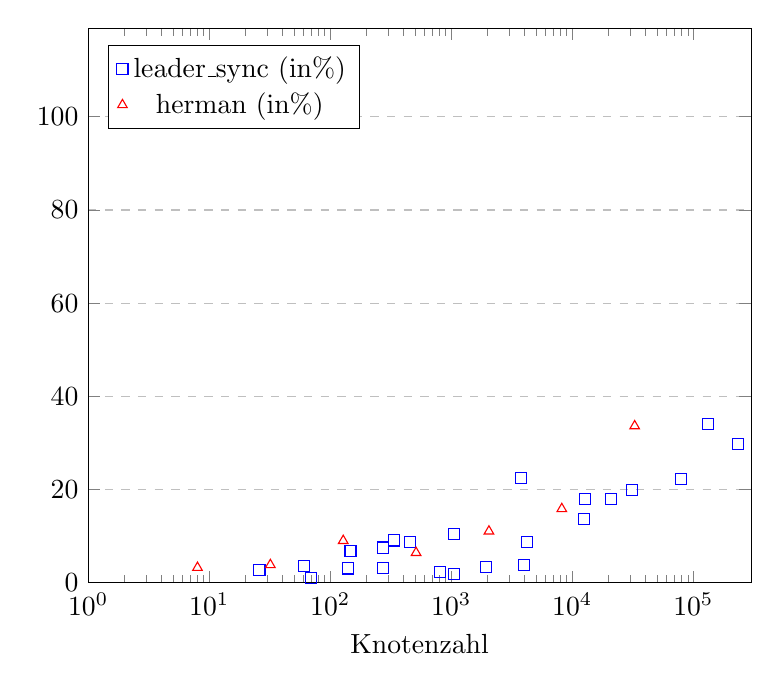
\begin{tikzpicture}
	\begin{axis}[
	xlabel={Knotenzahl},
	ylabel={},
	xmin=1,
	xmax=300000,
	xmode=log,
	ymin= 0,
	ymax=119,
	legend pos=north west,
	ymajorgrids=true,
	grid style=dashed,
	]
	\path[name path=axis] (axis cs:0,0) -- (axis cs:1,0);
	
	\addplot[only marks,color=blue,mark=square,name path=f]
	coordinates {
		(26,2.67611)(69,1.07258)(147,6.86191)(273,3.19697)(459,8.75836)(1059,10.4867)(61,3.54258)(274,7.57724)(812,2.23732)(1933,3.37525)(3962,3.85906)(12400,13.7232)(141,3.08846)(1050,1.81628)(4244,8.80112)(12709,17.9073)(31383,19.9319)(131521,34.0795)(335,9.10178)(3759,22.5585)(20884,17.9386)(78784,22.3324)(234210,29.7717)
	};
	
	\addplot[only marks,color=red,mark=triangle,name path=f]
	coordinates {
		(8,3.27121)(32,3.86944)(128,9.04134)(512,6.46046)(2048,11.0673)(8192,15.8791)(32768,33.6493)
	};
	
	\addlegendentry{leader\_sync (in\%)}
	\addlegendentry{herman (in\%)}
	\end{axis}
	\end{tikzpicture}
\end{figure}

% Kantenzahl in Abhängigkeit der Knotenzahl.

\begin{figure}
	\caption{Kantenzahl in Abhängigkeit der Knotenzahl}
	\label{fig-leader-sync}
	\centering
	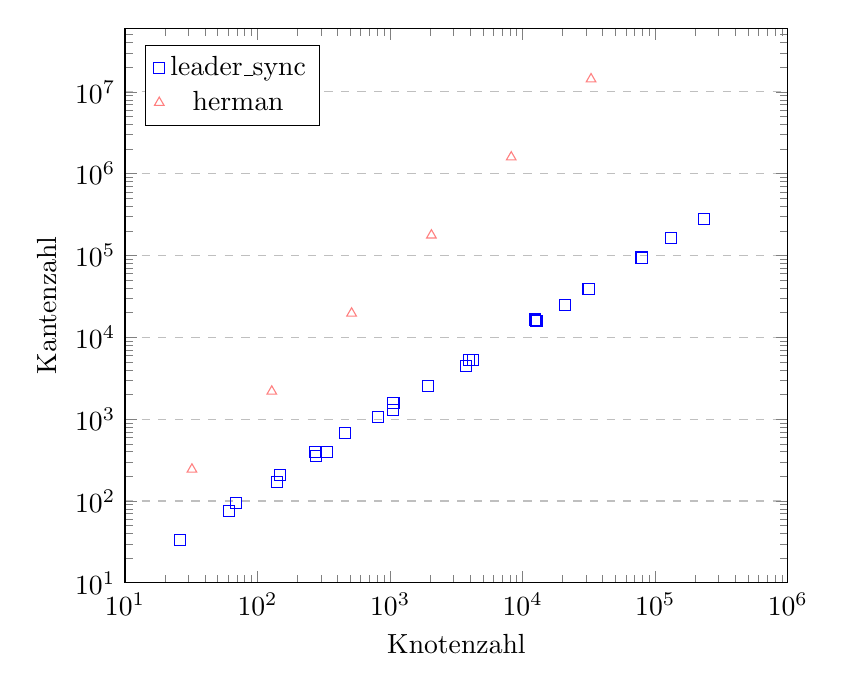
\begin{tikzpicture}
	\begin{axis}[
	xlabel={Knotenzahl},
	ylabel={Kantenzahl},
	xmin=10,
	xmax=1000000,
	xmode=log,
	ymin= 10,
	ymax=60000000,
	ymode=log,
	legend pos=north west,
	ymajorgrids=true,
	grid style=dashed,
	]
	\path[name path=axis] (axis cs:0,0) -- (axis cs:1,0);
	
	\addplot[only marks,color=blue,mark=square,name path=f]
	coordinates {
		(26,33)(69,95)(147,210)(273,397)(459,674)(1059,1570)(61,76)(274,354)(812,1067)(1933,2557)(3962,5257)(12400,16495)(141,172)(1050,1292)(4244,5267)(12709,15833)(31383,39158)(131521,164288)(335,398)(3759,4487)(20884,24979)(78784,94408)(234210,280865)
	};
	
	\addplot[only marks,color=red!50,mark=triangle,]
	coordinates {
		(8,28)(32,244)(128,2188)(512,19684)(2048,177148)(8192,1594324)(32768,14348908)
	};
	
	\addlegendentry{leader\_sync}
	\addlegendentry{herman}
	
	\end{axis}
	\end{tikzpicture}
\end{figure}

% time_solve_linear_system @ size_edges

\begin{figure}
	\caption{Zeitaufwand in Abhängigkeit der Kantenzahl}
	\label{fig-in-edges}
	\centering
	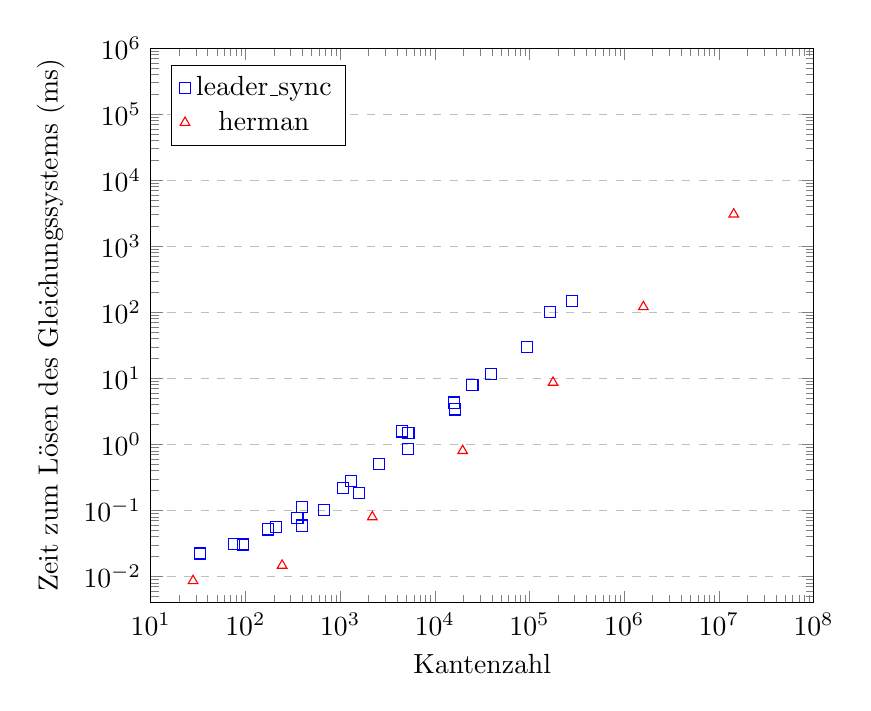
\begin{tikzpicture}
	\begin{axis}[
	xlabel={Kantenzahl},
	ylabel={Zeit zum Lösen des Gleichungssystems (ms) },
	xmin=10,
	xmax=100000000,
	xmode=log,
	ymode=log,
	ymin= 0.004,
	ymax=1000000,
	legend pos=north west,
	ymajorgrids=true,
	grid style=dashed,
	]
	\path[name path=axis] (axis cs:0,0) -- (axis cs:1,0);
	
	\addplot[ only marks,color=blue,mark=square,name path=f]
	coordinates {
		(33,0.0223)(95,0.0305)(210,0.0567)(397,0.059)(674,0.1008)(1570,0.1827)(76,0.030699999999999998)(354,0.0775)(1067,0.2203)(2557,0.5092)(5257,0.8613999999999999)(16495,3.3837)(172,0.051500000000000004)(1292,0.2766)(5267,1.4763)(15833,4.3047)(39158,11.5403)(164288,101.639)(398,0.1142)(4487,1.5696)(24979,7.9129)(94408,29.7813)(280865,149.87)
	};
	
	\addplot[only marks,color=red,mark=triangle,name path=f]
	coordinates {
		(28,0.0086)(244,0.0147)(2188,0.0796)(19684,0.8012)(177148,8.66)(1594324,120.8812)(14348908,3060.3275999999996)
	};
	
	\addlegendentry{leader\_sync}
	\addlegendentry{herman}
	\end{axis}
	\end{tikzpicture}
\end{figure}


\begin{figure}
	\caption{Zeitaufwand in Abhängigkeit der Kantenzahl}
	\label{fig-in-edges}
	\centering
	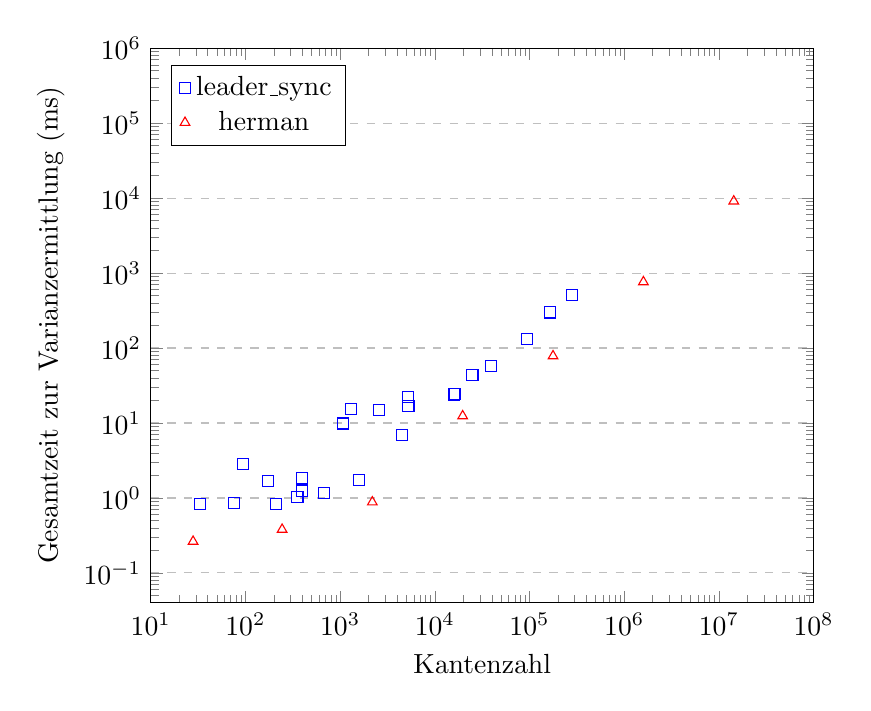
\begin{tikzpicture}
	\begin{axis}[
	xlabel={Kantenzahl},
	ylabel={Gesamtzeit zur Varianzermittlung (ms) },
	xmin=10,
	xmax=100000000,
	xmode=log,
	ymode=log,
	ymin= 0.04,
	ymax=1000000,
	legend pos=north west,
	ymajorgrids=true,
	grid style=dashed,
	]
	\path[name path=axis] (axis cs:0,0) -- (axis cs:1,0);
	
	\addplot[ only marks,color=blue,mark=square,name path=f]
	coordinates {
		(33,0.8333)(95,2.8436)(210,0.8263)(397,1.8455)(674,1.1509)(1570,1.7422)(76,0.8666)(354,1.0228)(1067,9.8466)(2557,15.0863)(5257,22.3215)(16495,24.6567)(172,1.6675)(1292,15.2289)(5267,16.774)(15833,24.0388)(39158,57.8987)(164288,298.241)(398,1.2547)(4487,6.9579)(24979,44.111)(94408,133.3549)(280865,503.3981)
	};
	
	\addplot[only marks,color=red,mark=triangle,name path=f]
	coordinates {
		(28,0.2629)(244,0.3799)(2188,0.8804)(19684,12.4016)(177148,78.2484)(1594324,761.2596)(14348908,9094.7637)
	};
	
	\addlegendentry{leader\_sync}
	\addlegendentry{herman}
	\end{axis}
	\end{tikzpicture}
\end{figure}


% percentage les_time/total_time @ size_nodes

\begin{figure}
	\caption{Anteil Lösung des Gleichungssystem an Gesamtzeitaufwand}
	\centering
	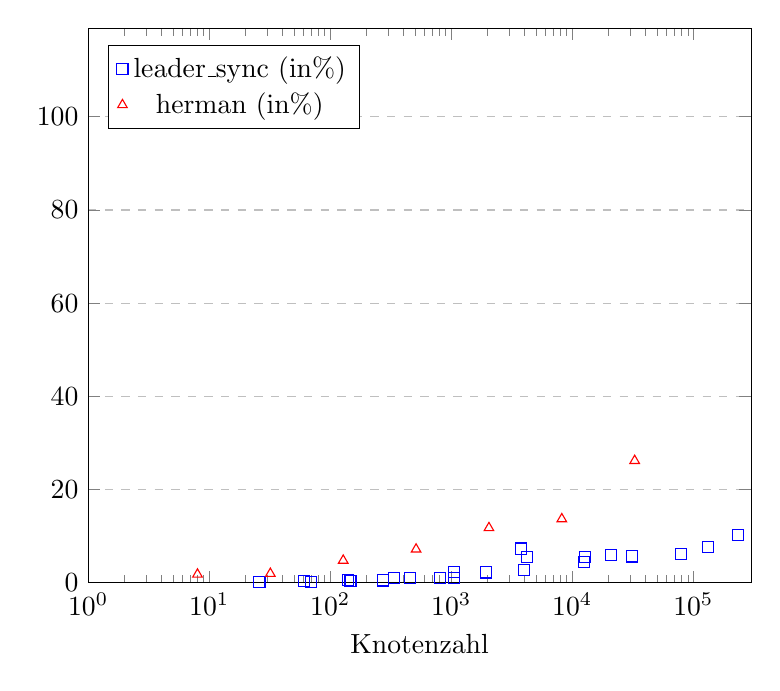
\begin{tikzpicture}
	\begin{axis}[
	xlabel={Knotenzahl},
	ylabel={},
	xmin=1,
	xmax=300000,
	xmode=log,
	ymin= 0,
	ymax=119,
	legend pos=north west,
	ymajorgrids=true,
	grid style=dashed,
	]
	\path[name path=axis] (axis cs:0,0) -- (axis cs:1,0);
	
	\addplot[only marks,color=blue,mark=square,name path=f]
	coordinates {
		(26,0.138194)(69,0.206001)(147,0.407508)(273,0.639828)(459,0.999371)(1059,1.11811)(61,0.354954)(274,0.510198)(812,0.971786)(1933,2.23148)(3962,2.70597)(12400,4.48214)(141,0.582958)(1050,2.35291)(4244,5.61032)(12709,5.49202)(31383,5.66286)(131521,7.63201)(335,1.08547)(3759,7.35931)(20884,5.93507)(78784,6.11997)(234210,10.2275)
	};
	
	\addplot[only marks,color=red,mark=triangle,name path=f]
	coordinates {
		(8,1.81928)(32,1.98175)(128,4.80159)(512,7.2)(2048,11.7886)(8192,13.6993)(32768,26.205)
	};
	
	\addlegendentry{leader\_sync (in\%)}
	\addlegendentry{herman (in\%)}
	\end{axis}
	\end{tikzpicture}
\end{figure}

% Kantenzahl in Abhängigkeit der Knotenzahl.

\begin{figure}
	\caption{Kantenzahl in Abhängigkeit der Knotenzahl}
	\label{fig-leader-sync}
	\centering
	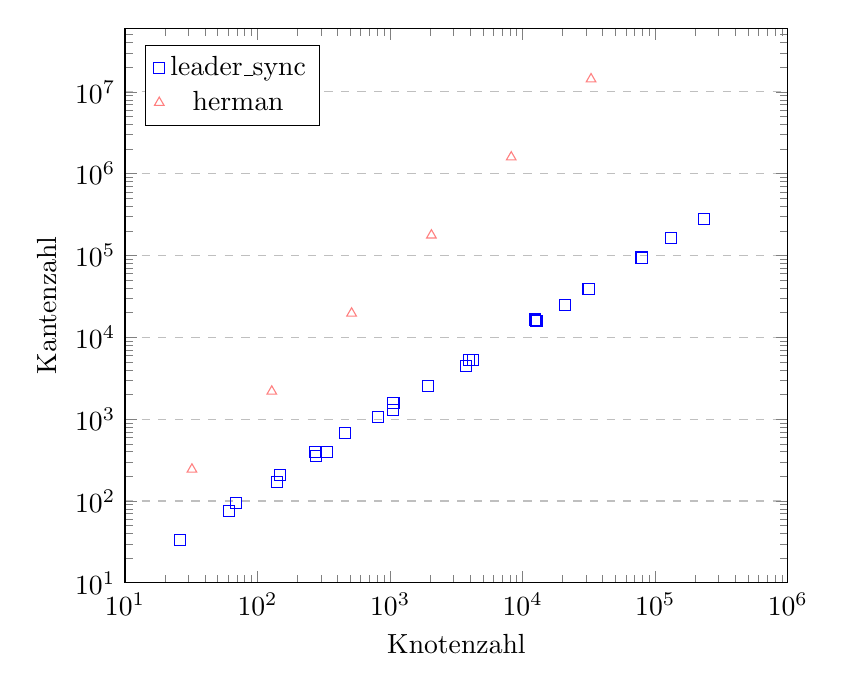
\begin{tikzpicture}
	\begin{axis}[
	xlabel={Knotenzahl},
	ylabel={Kantenzahl},
	xmin=10,
	xmax=1000000,
	xmode=log,
	ymin= 10,
	ymax=60000000,
	ymode=log,
	legend pos=north west,
	ymajorgrids=true,
	grid style=dashed,
	]
	\path[name path=axis] (axis cs:0,0) -- (axis cs:1,0);
	
	\addplot[only marks,color=blue,mark=square,name path=f]
	coordinates {
		(26,33)(69,95)(147,210)(273,397)(459,674)(1059,1570)(61,76)(274,354)(812,1067)(1933,2557)(3962,5257)(12400,16495)(141,172)(1050,1292)(4244,5267)(12709,15833)(31383,39158)(131521,164288)(335,398)(3759,4487)(20884,24979)(78784,94408)(234210,280865)
	};
	
	\addplot[only marks,color=red!50,mark=triangle,]
	coordinates {
		(8,28)(32,244)(128,2188)(512,19684)(2048,177148)(8192,1594324)(32768,14348908)
	};
	
	\addlegendentry{leader\_sync}
	\addlegendentry{herman}
	
	\end{axis}
	\end{tikzpicture}
\end{figure}

% time_solve_linear_system @ size_edges

\begin{figure}
	\caption{Zeitaufwand in Abhängigkeit der Kantenzahl}
	\label{fig-in-edges}
	\centering
	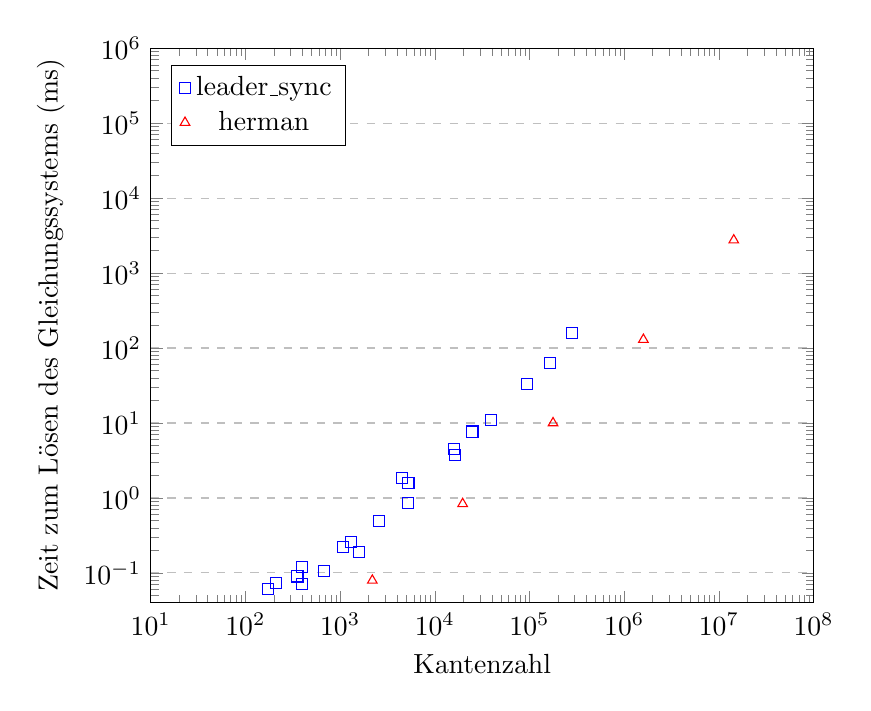
\begin{tikzpicture}
	\begin{axis}[
	xlabel={Kantenzahl},
	ylabel={Zeit zum Lösen des Gleichungssystems (ms) },
	xmin=10,
	xmax=100000000,
	xmode=log,
	ymode=log,
	ymin= 0.04,
	ymax=1000000,
	legend pos=north west,
	ymajorgrids=true,
	grid style=dashed,
	]
	\path[name path=axis] (axis cs:0,0) -- (axis cs:1,0);
	
	\addplot[ only marks,color=blue,mark=square,name path=f]
	coordinates {
		(33,0.0216)(95,0.034600000000000006)(210,0.0741)(397,0.07189999999999999)(674,0.1048)(1570,0.1913)(76,0.037000000000000005)(354,0.0897)(1067,0.2193)(2557,0.4954)(5257,0.8518)(16495,3.7192999999999996)(172,0.0618)(1292,0.25670000000000004)(5267,1.5782)(15833,4.5138)(39158,10.9094)(164288,63.343199999999996)(398,0.11979999999999999)(4487,1.8374000000000001)(24979,7.6944)(94408,32.8138)(280865,158.54410000000001)
	};
	
	\addplot[only marks,color=red,mark=triangle,name path=f]
	coordinates {
		(28,0.009)(244,0.0152)(2188,0.07949999999999999)(19684,0.8361000000000001)(177148,9.997399999999999)(1594324,129.5639)(14348908,2748.1414)
	};
	
	\addlegendentry{leader\_sync}
	\addlegendentry{herman}
	\end{axis}
	\end{tikzpicture}
\end{figure}

% time_solve_linear_system @ size_edges

\begin{figure}
	\caption{Zeitaufwand in Abhängigkeit der Kantenzahl}
	\label{fig-in-edges}
	\centering
	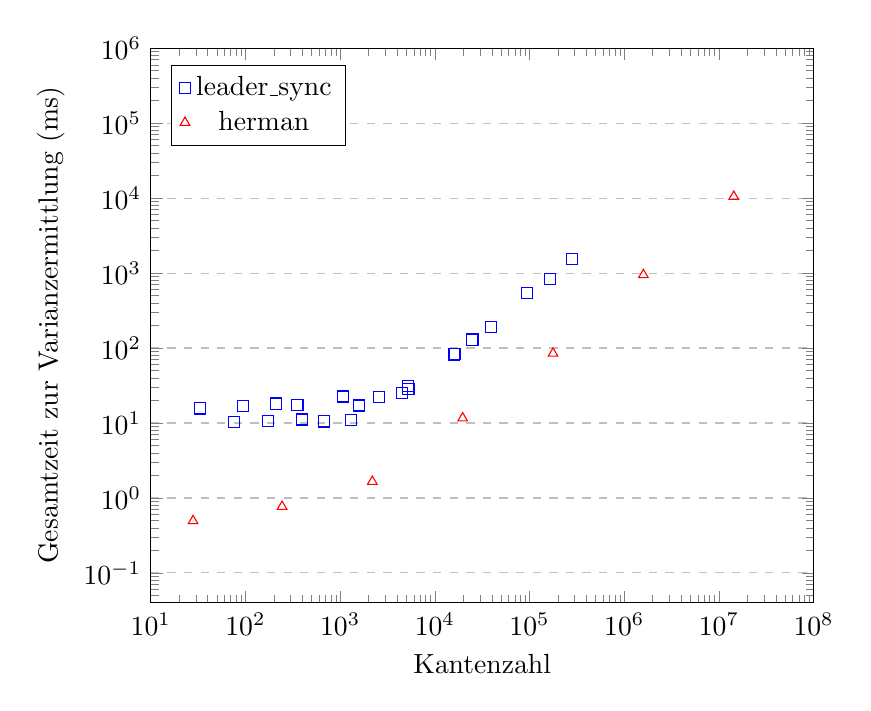
\begin{tikzpicture}
	\begin{axis}[
	xlabel={Kantenzahl},
	ylabel={Gesamtzeit zur Varianzermittlung (ms) },
	xmin=10,
	xmax=100000000,
	xmode=log,
	ymode=log,
	ymin= 0.04,
	ymax=1000000,
	legend pos=north west,
	ymajorgrids=true,
	grid style=dashed,
	]
	\path[name path=axis] (axis cs:0,0) -- (axis cs:1,0);
	
	\addplot[ only marks,color=blue,mark=square,name path=f]
	coordinates {
		(33,15.6302)(95,16.796)(210,18.1837)(397,11.2374)(674,10.4866)(1570,17.1093)(76,10.4239)(354,17.5814)(1067,22.5667)(2557,22.2005)(5257,31.4785)(16495,82.9805)(172,10.6011)(1292,10.9099)(5267,28.1303)(15833,82.1884)(39158,192.6484)(164288,829.9677)(398,11.0367)(4487,24.967)(24979,129.6429)(94408,536.1761)(280865,1550.1791)
	};
	
	\addplot[only marks,color=red,mark=triangle,name path=f]
	coordinates {
		(28,0.4947)(244,0.767)(2188,1.6557)(19684,11.6125)(177148,84.8055)(1594324,945.7732)(14348908,10487.1059)
	};
	
	\addlegendentry{leader\_sync}
	\addlegendentry{herman}
	\end{axis}
	\end{tikzpicture}
\end{figure}


% optimiertes eigen nmit bicgstab:
% percentage les_time/total_time @ size_nodes

\begin{figure}
	\caption{Anteil Lösung des Gleichungssystem an Gesamtzeitaufwand}
	\centering
	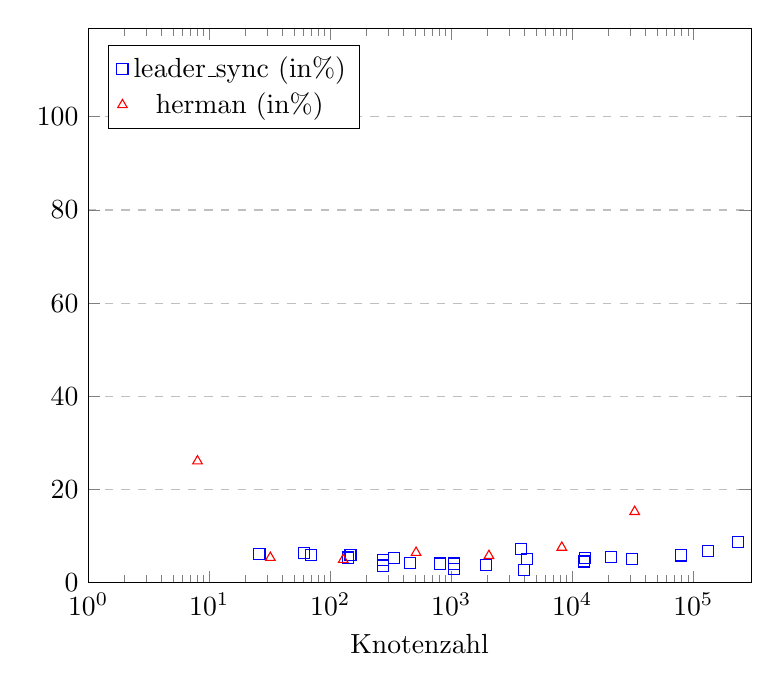
\begin{tikzpicture}
	\begin{axis}[
	xlabel={Knotenzahl},
	ylabel={},
	xmin=1,
	xmax=300000,
	xmode=log,
	ymin= 0,
	ymax=119,
	legend pos=north west,
	ymajorgrids=true,
	grid style=dashed,
	]
	\path[name path=axis] (axis cs:0,0) -- (axis cs:1,0);
	
	\addplot[only marks,color=blue,mark=square,name path=f]
	coordinates {
		(26,6.22407)(69,5.92593)(147,5.91537)(273,3.71022)(459,4.25576)(1059,2.93305)(61,6.41302)(274,4.88163)(812,4.13457)(1933,3.89433)(3962,2.82031)(12400,4.57664)(141,5.41817)(1050,4.14424)(4244,5.07803)(12709,5.34311)(31383,5.1597)(131521,6.7501)(335,5.3184)(3759,7.18407)(20884,5.59286)(78784,5.87375)(234210,8.71078)
	};
	
	\addplot[only marks,color=red,mark=triangle,name path=f]
	coordinates {
		(8,26.1062)(32,5.40654)(128,4.97245)(512,6.48853)(2048,5.8165)(8192,7.59112)(32768,15.2671)
	};
	
	\addlegendentry{leader\_sync (in\%)}
	\addlegendentry{herman (in\%)}
	\end{axis}
	\end{tikzpicture}
\end{figure}

% Kantenzahl in Abhängigkeit der Knotenzahl.

\begin{figure}
	\caption{Kantenzahl in Abhängigkeit der Knotenzahl}
	\label{fig-leader-sync}
	\centering
	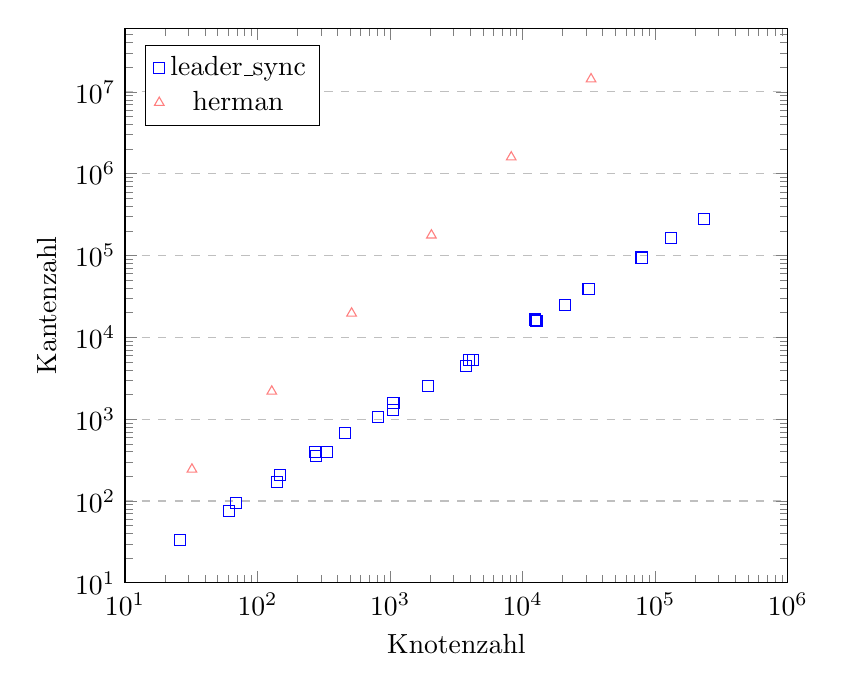
\begin{tikzpicture}
	\begin{axis}[
	xlabel={Knotenzahl},
	ylabel={Kantenzahl},
	xmin=10,
	xmax=1000000,
	xmode=log,
	ymin= 10,
	ymax=60000000,
	ymode=log,
	legend pos=north west,
	ymajorgrids=true,
	grid style=dashed,
	]
	\path[name path=axis] (axis cs:0,0) -- (axis cs:1,0);
	
	\addplot[only marks,color=blue,mark=square,name path=f]
	coordinates {
		(26,33)(69,95)(147,210)(273,397)(459,674)(1059,1570)(61,76)(274,354)(812,1067)(1933,2557)(3962,5257)(12400,16495)(141,172)(1050,1292)(4244,5267)(12709,15833)(31383,39158)(131521,164288)(335,398)(3759,4487)(20884,24979)(78784,94408)(234210,280865)
	};
	
	\addplot[only marks,color=red!50,mark=triangle,]
	coordinates {
		(8,28)(32,244)(128,2188)(512,19684)(2048,177148)(8192,1594324)(32768,14348908)
	};
	
	\addlegendentry{leader\_sync}
	\addlegendentry{herman}
	
	\end{axis}
	\end{tikzpicture}
\end{figure}

% time_solve_linear_system @ size_edges

\begin{figure}
	\caption{Zeitaufwand in Abhängigkeit der Kantenzahl}
	\label{fig-in-edges}
	\centering
	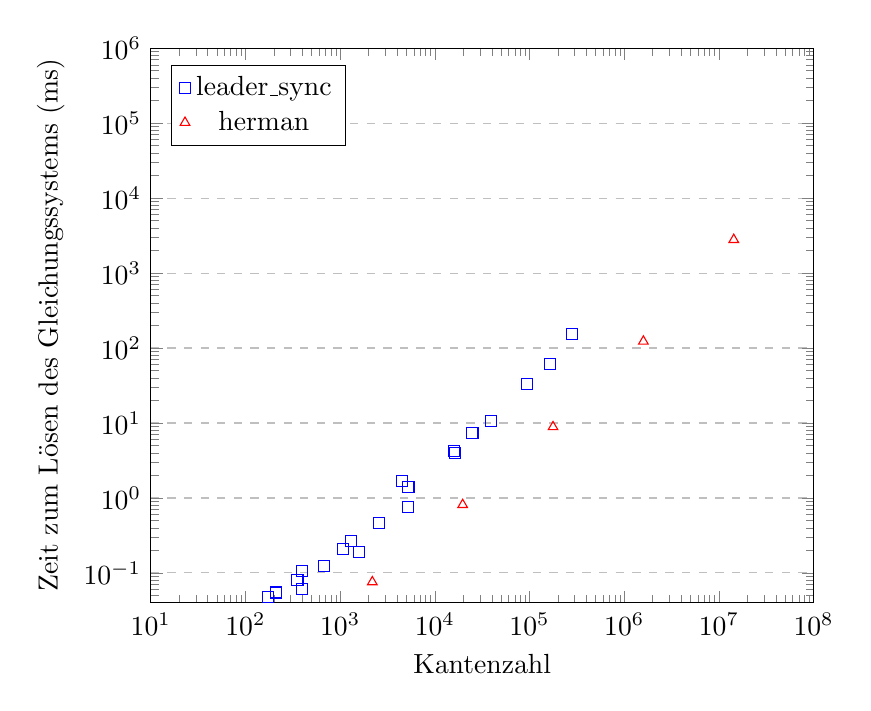
\begin{tikzpicture}
	\begin{axis}[
	xlabel={Kantenzahl},
	ylabel={Zeit zum Lösen des Gleichungssystems (ms) },
	xmin=10,
	xmax=100000000,
	xmode=log,
	ymode=log,
	ymin= 0.04,
	ymax=1000000,
	legend pos=north west,
	ymajorgrids=true,
	grid style=dashed,
	]
	\path[name path=axis] (axis cs:0,0) -- (axis cs:1,0);
	
	\addplot[ only marks,color=blue,mark=square,name path=f]
	coordinates {
		(33,0.013500000000000002)(95,0.028)(210,0.0548)(397,0.061200000000000004)(674,0.124)(1570,0.19)(76,0.026799999999999997)(354,0.0798)(1067,0.2072)(2557,0.4589)(5257,0.7631)(16495,3.9668)(172,0.0482)(1292,0.2672)(5267,1.4141)(15833,4.2649)(39158,10.499500000000001)(164288,60.887699999999995)(398,0.1059)(4487,1.6795)(24979,7.395300000000001)(94408,33.5254)(280865,152.9287)
	};
	
	\addplot[only marks,color=red,mark=triangle,name path=f]
	coordinates {
		(28,0.0059)(244,0.0129)(2188,0.0758)(19684,0.8118)(177148,8.8644)(1594324,122.7962)(14348908,2787.7731)
	};
	
	\addlegendentry{leader\_sync}
	\addlegendentry{herman}
	\end{axis}
	\end{tikzpicture}
\end{figure}

% time_solve_linear_system @ size_edges




% optimiertes eigen mit conjugate gradtiebnd
% percentage les_time/total_time @ size_nodes

\begin{figure}
	\caption{Anteil Lösung des Gleichungssystem an Gesamtzeitaufwand}
	\centering
	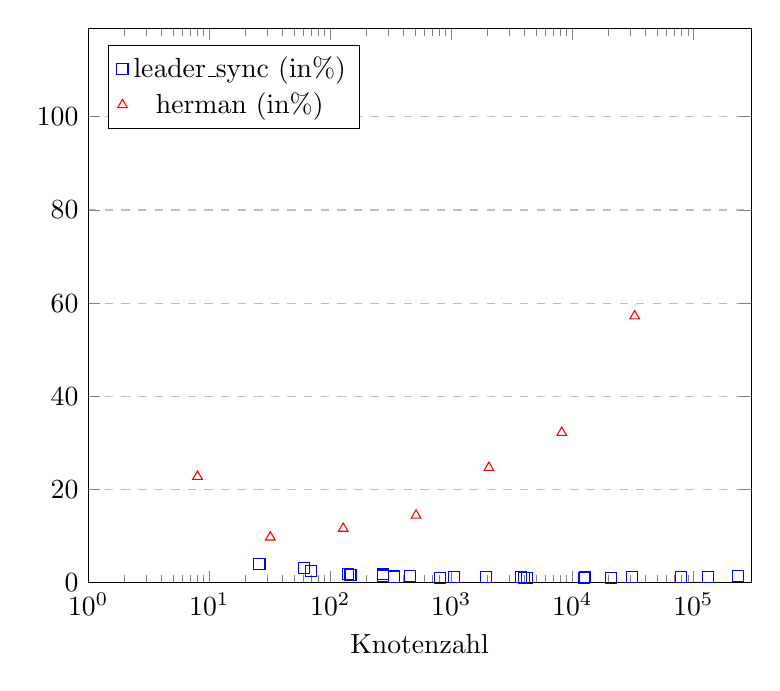
\begin{tikzpicture}
	\begin{axis}[
	xlabel={Knotenzahl},
	ylabel={},
	xmin=1,
	xmax=300000,
	xmode=log,
	ymin= 0,
	ymax=119,
	legend pos=north west,
	ymajorgrids=true,
	grid style=dashed,
	]
	\path[name path=axis] (axis cs:0,0) -- (axis cs:1,0);
	
	\addplot[only marks,color=blue,mark=square,name path=f]
	coordinates {
		(26,4.06279)(69,2.61079)(147,1.76563)(273,1.56044)(459,1.41541)(1059,1.23112)(61,3.23054)(274,1.86073)(812,1.08651)(1933,1.27822)(3962,1.00628)(12400,0.95026)(141,1.85468)(1050,1.26343)(4244,1.05124)(12709,1.19792)(31383,1.17696)(131521,1.2659)(335,1.34578)(3759,1.28221)(20884,1.0144)(78784,1.17595)(234210,1.44043)
	};
	
	\addplot[only marks,color=red,mark=triangle,name path=f]
	coordinates {
		(8,22.807)(32,9.79499)(128,11.6553)(512,14.489)(2048,24.7196)(8192,32.2307)(32768,57.2231)
	};
	
	\addlegendentry{leader\_sync (in\%)}
	\addlegendentry{herman (in\%)}
	\end{axis}
	\end{tikzpicture}
\end{figure}

% Kantenzahl in Abhängigkeit der Knotenzahl.

\begin{figure}
	\caption{Kantenzahl in Abhängigkeit der Knotenzahl}
	\label{fig-leader-sync}
	\centering
	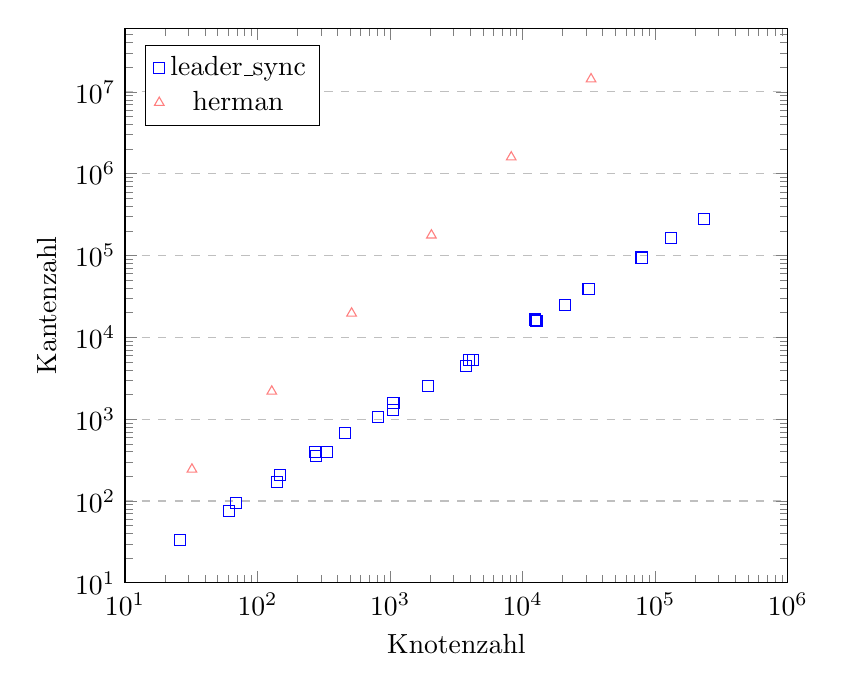
\begin{tikzpicture}
	\begin{axis}[
	xlabel={Knotenzahl},
	ylabel={Kantenzahl},
	xmin=10,
	xmax=1000000,
	xmode=log,
	ymin= 10,
	ymax=60000000,
	ymode=log,
	legend pos=north west,
	ymajorgrids=true,
	grid style=dashed,
	]
	\path[name path=axis] (axis cs:0,0) -- (axis cs:1,0);
	
	\addplot[only marks,color=blue,mark=square,name path=f]
	coordinates {
		(26,33)(69,95)(147,210)(273,397)(459,674)(1059,1570)(61,76)(274,354)(812,1067)(1933,2557)(3962,5257)(12400,16495)(141,172)(1050,1292)(4244,5267)(12709,15833)(31383,39158)(131521,164288)(335,398)(3759,4487)(20884,24979)(78784,94408)(234210,280865)
	};
	
	\addplot[only marks,color=red!50,mark=triangle,]
	coordinates {
		(8,28)(32,244)(128,2188)(512,19684)(2048,177148)(8192,1594324)(32768,14348908)
	};
	
	\addlegendentry{leader\_sync}
	\addlegendentry{herman}
	
	\end{axis}
	\end{tikzpicture}
\end{figure}

% time_solve_linear_system @ size_edges

\begin{figure}
	\caption{Zeitaufwand in Abhängigkeit der Kantenzahl}
	\label{fig-in-edges}
	\centering
	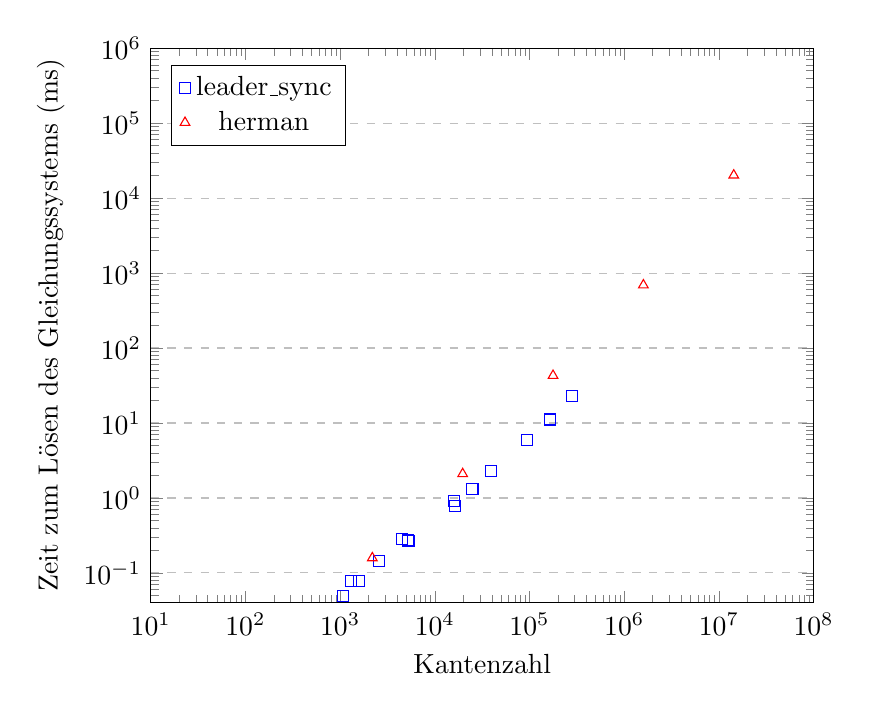
\begin{tikzpicture}
	\begin{axis}[
	xlabel={Kantenzahl},
	ylabel={Zeit zum Lösen des Gleichungssystems (ms) },
	xmin=10,
	xmax=100000000,
	xmode=log,
	ymode=log,
	ymin= 0.04,
	ymax=1000000,
	legend pos=north west,
	ymajorgrids=true,
	grid style=dashed,
	]
	\path[name path=axis] (axis cs:0,0) -- (axis cs:1,0);
	
	\addplot[ only marks,color=blue,mark=square,name path=f]
	coordinates {
		(33,0.0088)(95,0.0119)(210,0.0157)(397,0.0248)(674,0.0375)(1570,0.0789)(76,0.0132)(354,0.029900000000000003)(1067,0.0497)(2557,0.14250000000000002)(5257,0.2757)(16495,0.7723)(172,0.0158)(1292,0.07880000000000001)(5267,0.2663)(15833,0.9169)(39158,2.285)(164288,11.129999999999999)(398,0.0258)(4487,0.2835)(24979,1.3282)(94408,5.9991)(280865,22.6284)
	};
	
	\addplot[only marks,color=red,mark=triangle,name path=f]
	coordinates {
		(28,0.005200000000000001)(244,0.0258)(2188,0.1585)(19684,2.1002)(177148,42.942099999999996)(1594324,691.395)(14348908,20202.6659)
	};
	
	\addlegendentry{leader\_sync}
	\addlegendentry{herman}
	\end{axis}
	\end{tikzpicture}
\end{figure}

% time_solve_linear_system @ size_edges

\begin{figure}
	\caption{Zeitaufwand in Abhängigkeit der Kantenzahl}
	\label{fig-in-edges}
	\centering
	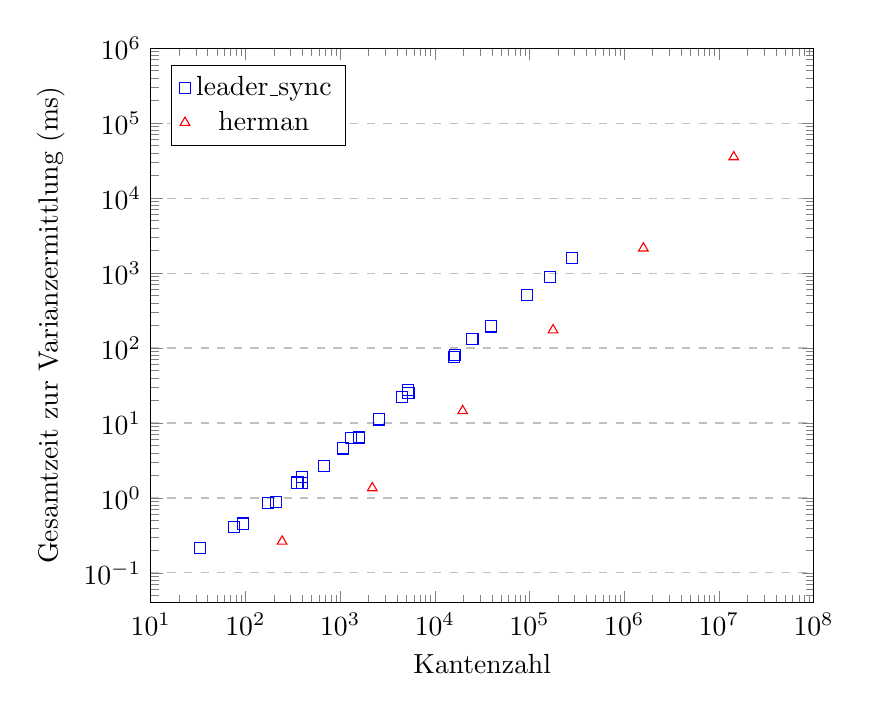
\begin{tikzpicture}
	\begin{axis}[
	xlabel={Kantenzahl},
	ylabel={Gesamtzeit zur Varianzermittlung (ms) },
	xmin=10,
	xmax=100000000,
	xmode=log,
	ymode=log,
	ymin= 0.04,
	ymax=1000000,
	legend pos=north west,
	ymajorgrids=true,
	grid style=dashed,
	]
	\path[name path=axis] (axis cs:0,0) -- (axis cs:1,0);
	
	\addplot[ only marks,color=blue,mark=square,name path=f]
	coordinates {
		(33,0.2166)(95,0.4558)(210,0.8892)(397,1.5893)(674,2.6494)(1570,6.4088)(76,0.4086)(354,1.6069)(1067,4.5743)(2557,11.1483)(5257,27.398)(16495,81.2725)(172,0.8519)(1292,6.237)(5267,25.332)(15833,76.5412)(39158,194.1443)(164288,879.2178)(398,1.9171)(4487,22.1102)(24979,130.9343)(94408,510.1477)(280865,1570.9472)
	};
	
	\addplot[only marks,color=red,mark=triangle,name path=f]
	coordinates {
		(28,0.0228)(244,0.2634)(2188,1.3599)(19684,14.4951)(177148,173.7169)(1594324,2145.145)(14348908,35305.0664)
	};
	
	\addlegendentry{leader\_sync}
	\addlegendentry{herman}
	\end{axis}
	\end{tikzpicture}
\end{figure}
\end{comment}
\section{Appendix}

Wir wollen nachfolgend solche mathematische Aussagen kurz darlegen und begründen, die nicht zentrales Thema dieser Arbeit sind, jedoch an bestimmten Stellen zur Argumentation herangezogen werden.

\begin{lemma} \label{lem-geosum}
	Seien $n \in \mathbb{N}$ eine natürliche Zahl und $a \in \mathbb{R}_{>0}\setminus\{1\}$. Dann gilt
\begin{equation}
\sum_{i=0}^{n}{a^i} = \frac{a^{n+1}-1}{a-1}
\end{equation}
\end{lemma}
\begin{beweis}
\begin{align*}
	(a-1) \cdot \sum_{i=0}^{n}{a^i} = \sum_{i=0}^{n}{a^{i+1}} - \sum_{i=0}^{n}{a^i} = a^{n+1} - 1
\end{align*}
\end{beweis}

\begin{korollar} \label{kor-geosum}
Betrachten wir den Grenzwert der Summe aus Lemma \ref{lem-geosum} für $n \to \infty$, so ergibt sich für $0<a<1$:
\begin{equation}
\sum_{i=0}^{\infty}{a^i}
= \lim\limits_{n \to \infty} \sum_{i=0}^{n}{a^i}
= \frac{1}{1-a}
\end{equation}
\end{korollar}

\begin{lemma} \label{lem-infsum}
	Seien $n \in \mathbb{N}$ eine natürliche Zahl und $a \in \mathbb{R}_{>0}\setminus\{1\}$. Dann gilt
	\begin{equation}
		\sum_{i=0}^{n}{i\cdot a^i} = \frac{(an-n-1)a^{n+1}+a}{(a-1)^2}
	\end{equation}
\end{lemma}
\begin{beweis}
	\begin{align*}
		&(n+1) a^{n+1} + \sum_{i=0}^{n}{i\cdot a^i} = \sum_{i=0}^{n+1}{i\cdot a^i} = \sum_{i=0}^{n}{(i+1)\cdot a^{i+1}} \\
		=& a \sum_{i=0}^{n}{i\cdot a^{i}} + a \sum_{i=0}^{n}{a^{i}} = a \sum_{i=0}^{n}{i\cdot a^{i}} + a \cdot \frac{a^{n+1}-1}{a-1}\\
		\Rightarrow \quad & (a-1) \sum_{i=0}^{n}{i\cdot a^i} = (n+1) a^{n+1} - a \cdot \frac{a^{n+1}-1}{a-1} 
	\end{align*}
\end{beweis}
\begin{korollar} \label{kor-infsum}
Betrachten wir den Grenzwert der Summe aus Lemma \ref{lem-infsum} für $n \to \infty$, so ergibt sich für $0<a<1$:
\begin{equation}
\sum_{i=0}^{\infty}{i\cdot a^i}
= \lim\limits_{n \to \infty} \sum_{i=0}^{n}{i\cdot a^i}
= \frac{a}{(a-1)^2}
\end{equation}
\end{korollar}

\begin{lemma} \label{lem-infqsum}
	Seien $n \in \mathbb{N}$ eine natürliche Zahl und $a \in \mathbb{R}_{>0}\setminus\{1\}$. Dann gilt
	\begin{equation}
	\sum_{i=0}^{n}{i^2\cdot a^i} = \frac{\big(-a^2n^2 + a(2n^2 + 2n + 1) - (n+1)^2\big)a^{n+1}+a(a+1)}{(a-1)^3}
	\end{equation}
\end{lemma}
\begin{beweis}
	\begin{align*}
		 & n^2a^n + \sum_{i=0}^{n-1}{i^2\cdot a^i} = \sum_{i=0}^{n}{i^2\cdot a^i} = \sum_{i=0}^{n-1}{(i+1)^2\cdot a^{i+1}} \\
		=& a \sum_{i=0}^{n-1}{i^2\cdot a^{i}} + 2a \sum_{i=0}^{n-1}{i\cdot a^{i}} + a \sum_{i=0}^{n-1}{ a^{i}} \\
		=& a \left(\sum_{i=0}^{n}{i^2\cdot a^i} - n^2a^n \right) + 2a \left(\frac{(an-a-n)a^{n}+a}{(a-1)^2} \right) + a \left( \frac{a^{n}-1}{a-1} \right) \\
		\Rightarrow \quad & (1-a) \sum_{i=0}^{n}{i^2\cdot a^i} = -n^2a^{n+1} + 2a \left(\frac{(an-a-n)a^{n}+a}{(a-1)^2} \right) + a \left( \frac{a^{n}-1}{a-1} \right)
	\end{align*}
\end{beweis}
\begin{korollar} \label{kor-infqsum}
Betrachten wir den Grenzwert der Summe aus Lemma \ref{lem-infqsum} für $n \to \infty$, so ergibt sich für $0<a<1$:
\begin{equation}
\sum_{i=0}^{\infty}{i^2\cdot a^i}
= \lim\limits_{n \to \infty} \sum_{i=0}^{n}{i^2\cdot a^i}
= \frac{a\;(a+1)}{(1-a)^3}
\end{equation}	
\end{korollar}

\printbibliography

\end{document}